\documentclass[honours,12pt, twoside]{unswthesis}
\linespread{1.3}
\usepackage{kotex}
\usepackage{amsfonts}
\usepackage{subcaption}
\captionsetup{compatibility=false}
\usepackage{appendix}
\usepackage{bbm}
\usepackage{multirow}
\usepackage{amssymb}
\usepackage{hyperref}
\renewcommand{\chapterautorefname}{Chapter}
\renewcommand{\sectionautorefname}{Section}
\renewcommand{\subsectionautorefname}{Subsection}
\def\appendixautorefname{Appendix}

% begin appendix autoref patch [\autoref subsections in appendix](https://tex.stackexchange.com/questions/149807/autoref-subsections-in-appendix)
\usepackage{etoolbox}
\makeatletter
\patchcmd{\hyper@makecurrent}{%
    \ifx\Hy@param\Hy@chapterstring
        \let\Hy@param\Hy@chapapp
    \fi
}{%
    \iftoggle{inappendix}{%true-branch
        % list the names of all sectioning counters here
        \@checkappendixparam{chapter}%
        \@checkappendixparam{section}%
        \@checkappendixparam{subsection}%
        \@checkappendixparam{subsubsection}%
        \@checkappendixparam{paragraph}%
        \@checkappendixparam{subparagraph}%
    }{}%
}{}{\errmessage{failed to patch}}

\newcommand*{\@checkappendixparam}[1]{%
    \def\@checkappendixparamtmp{#1}%
    \ifx\Hy@param\@checkappendixparamtmp
        \let\Hy@param\Hy@appendixstring
    \fi
}
\makeatletter

\newtoggle{inappendix}
\togglefalse{inappendix}

\apptocmd{\appendix}{\toggletrue{inappendix}}{}{\errmessage{failed to patch}}
\apptocmd{\subappendices}{\toggletrue{inappendix}}{}{\errmessage{failed to patch}}
%\usepackage[nameinlink,capitalise]{cleveref}
\usepackage{amsthm}
\usepackage{latexsym,amsmath}
\usepackage{graphicx}
\usepackage{mathtools}
\usepackage{pgfplots}
\usepackage{afterpage}
\usepackage[ ]{algorithm2e}
\renewcommand{\algorithmautorefname}{Algorithm}
\usepackage{bm}
\usepackage{tikz}
\usetikzlibrary{bayesnet}
\usepackage{boondox-cal}
\usepackage{cite}
\usepackage[square]{natbib}
\allowdisplaybreaks[1]
%%%%%%%%%%%%%%%%%%%%%%%%%%%%%%%%%%%%%%%%%%%%%%%%%%%%%%%%%%%%%%%%%
%
%  The following are some simple LaTeX macros to give some
%  commonly used letters in funny fonts. You may need more or less of
%  these
%
\newcommand{\R}{\mathbb{R}}
\newcommand{\Q}{\mathbb{Q}}
\newcommand{\C}{\mathbb{C}}
\newcommand{\N}{\mathbb{N}}
\newcommand{\F}{\mathbb{F}}
\newcommand{\PP}{\mathbb{P}}
\newcommand{\T}{\mathbb{T}}
\newcommand{\Z}{\mathbb{Z}}
\newcommand{\B}{\mathfrak{B}}
\newcommand{\BB}{\mathcal{B}}
\newcommand{\M}{\mathfrak{M}}
\newcommand{\X}{\mathfrak{X}}
\newcommand{\Y}{\mathfrak{Y}}
\newcommand{\CC}{\mathcal{C}}
\newcommand{\E}{\mathbb{E}}
\newcommand{\cP}{\mathcal{P}}
\newcommand{\cS}{\mathcal{S}}
\newcommand{\A}{\mathcal{A}}
\newcommand{\ZZ}{\mathcal{Z}}
%%%%%%%%%%%%%%%%%%%%%%%%%%%%%%%%%%%%%%%%%%%%%%%%%%%%%%%%%%%%%%%%%%%%%
%
% The following are much more esoteric commands that I have left in
% so that this file still processes. Use or delete as you see fit
%
\newcommand{\var}{\mathop{\rm var}}
\newcommand{\Var}{\mathrm{Var}}
\newcommand{\ltp}{\mathrel{{\prec}_p}}
\newcommand{\lep}{\mathrel{{\preceq}_p}}
\def\brack#1{\left \{ #1 \right \}}
\def\bul{$\bullet$\ }
\def\cl{{\rm cl}}
\let\del=\partial
\def\enditem{\par\smallskip\noindent}
\def\implies{\Rightarrow}
\def\inpr#1,#2{\t \hbox{\langle #1 , #2 \rangle} \t}
\def\ip<#1,#2>{\langle #1,#2 \rangle}
\def\lp{\ell^p}
\def\maxb#1{\max \brack{#1}}
\def\minb#1{\min \brack{#1}}
\def\mod#1{\left \vert #1 \right \vert}
\def\norm#1{\left \Vert #1 \right \Vert}
\def\paren(#1){\left( #1 \right)}
\def\qed{\hfill \hbox{$\Box$} \smallskip}
\def\sbrack#1{\Bigl \{ #1 \Bigr \} }
\def\ssbrack#1{ \{ #1 \} }
\def\smod#1{\Bigl \vert #1 \Bigr \vert}
\def\smmod#1{\bigl \vert #1 \bigr \vert}
\def\ssmod#1{\vert #1 \vert}
\def\sspmod#1{\vert\, #1 \, \vert}
\def\snorm#1{\Bigl \Vert #1 \Bigr \Vert}
\def\ssnorm#1{\Vert #1 \Vert}
\def\sparen(#1){\Bigl ( #1 \Bigr )}
\DeclareMathOperator*{\argmin}{arg\,min}
\DeclareMathOperator*{\argmax}{arg\,max}
\DeclareMathOperator{\tr}{tr}
\newcommand\blankpage{%
    \null
    \thispagestyle{empty}%
    \addtocounter{page}{-1}%
    \newpage}

%%%%%%%%%%%%%%%%%%%%%%%%%%%%%%%%%%%%%%%%%%%%%%%%%%%%%%%%%%%%%%
%
% These environments allow you to get nice numbered headings
%  for your Theorems, Definitions etc.  
%
%  Environments
%
%%%%%%%%%%%%%%%%%%%%%%%%%%%%%%%

\newtheorem{theorem}{Theorem}[section]
\newtheorem{lemma}[theorem]{Lemma}
\newtheorem{proposition}[theorem]{Proposition}
\newtheorem{corollary}[theorem]{Corollary}
\newtheorem{conjecture}[theorem]{Conjecture}

\newtheorem{remark}[theorem]{Remark}
\newtheorem{question}[theorem]{Question}
\newtheorem{notation}[theorem]{Notation}
\numberwithin{equation}{section}
\theoremstyle{definition}
\newtheorem{definition}[theorem]{Definition}
\newtheorem{example}[theorem]{Example}
%%%%%%%%%%%%%%%%%%%%%%%%%%%%%%%%%%%%%%%%%%%%%%%%%%%%%%%%%%%%%%%%%%
%
%  If you've got some funny special words that LaTeX might not
% hyphenate properly, you can give it a helping hand:
%
\hyphenation{Mar-cin-kie-wicz Rade-macher}

%%%%%%%%%%%%%%%%%%%%%%%%%%%%%%%%%%%%%%%%%%%%%%%%%%%%%%%%%%%%%%%%%%
% 
% OK...Now we get to some actual input.  The first part sets up
% the title etc that will appear on the front page
%
%%%%%%%%%%%%%%%%%%%%%%%%%%%%%%%%%%%%%%%%%%%%%%%%%%%%%%%%%%%%%%%%%

\title{Density Ratio Estimation in Variational Bayesian Machine Learning}

\authornameonly{Alexander Lam}

\author{\Authornameonly\\{\bigskip}Supervisors: Professor Scott Sisson and Doctor Edwin Bonilla}

\copyrightfalse
\figurespagefalse
\tablespagefalse

%%%%%%%%%%%%%%%%%%%%%%%%%%%%%%%%%%%%%%%%%%%%%%%%%%%%%%%%%%%%%%%%%
%
%  And now the document begins
%  The \beforepreface and \afterpreface commands puts the
%  contents page etc in
%
%%%%%%%%%%%%%%%%%%%%%%%%%%%%%%%%%%%%%%%%%%%%%%%%%%%%%%%%%%%%%%%%%%

\begin{document}

\beforepreface

\afterpage{\clearpage}

% plagiarism

\prefacesection{Plagiarism statement}

\vskip 10pc \noindent I declare that this thesis is my
own work, except where acknowledged, and has not been submitted for
academic credit elsewhere. 

\vskip 2pc  \noindent I acknowledge that the assessor of this
thesis may, for the purpose of assessing it:
\begin{itemize}
\item Reproduce it and provide a copy to another member of the University; and/or,
\item Communicate a copy of it to a plagiarism checking service (which may then retain a copy of it on its database for the purpose of future plagiarism checking).
\end{itemize}

\vskip 2pc \noindent I certify that I have read and understood the University Rules in
respect of Student Academic Misconduct, and am aware of any potential plagiarism penalties which may 
apply.\vspace{24pt}

\vskip 2pc \noindent By signing 
this declaration I am
agreeing to the statements and conditions above.
\vskip 2pc \noindent
Signed: \rule{7cm}{0.25pt} \hfill Date: \rule{4cm}{0.25pt} \newline
\vskip 1pc

\afterpage{\cleardoublepage}

% Acknowledgements are optional


\prefacesection{Acknowledgements}

{\bigskip}By far my greatest thanks must go to my supervisors Scott Sisson and Edwin Bonilla for the care and support they provided throughout this year. I am very pleased that they have guided me through such a unique topic which spans the fields of applied mathematics, statistics and computer science. I would also like to thank Edwin's PhD student Louis Tiao for helping me with some crucial areas in this thesis.

{\bigskip\noindent}My second greatest thanks goes to my senior high school mathematics teacher Trevor Trotman. His passion and excellent teaching was crucial to helping me discover my enjoyment of mathematics. If not for him, I would have likely taken a more dull path in life.

{\bigskip\noindent}It is imperative that I express gratitude to the inhabitants of Red Center Room 3084 for accompanying and distracting me throughout this year. In particular, I would like to thank the senior inhabitants Prosha, Ramanan and Jeffrey for their constructive criticisms of my writing and presentation.

{\bigskip\noindent}Shout-out to the Discord fellas for entertaining me and encouraging me to pursue a career as a professional DJ. Extra shout-out to Davey cause he asked for one. Also shout-out to Kong for letting me leech off his gym pass.

{\bigskip\noindent}I would also like to acknowledge the help of Matthew for setting up my github, Sunchit for his Python tech support, and Allan for showing me that the Euler-Lagrange equation can be employed to find the second derivatives of my loss functionals.

{\bigskip\noindent}저를 돌보고 나를 응원해준 한채린누나에게 감사 드리고 싶습니다. 올해 가장 행복한 순간 중 일부는 그녀와 함께 보냈습니다. 저는 그런 친절하고 예쁜 누나를 가지고있어서 운이 좋습니다.

{\bigskip\noindent}Lastly, I would like to thank Jin, Eliza and Brian for encouraging me to be ambitious in all aspects of my future aspirations.

{\bigskip\bigskip\bigskip\noindent}Lammy, 25 October 2018.

\afterpage{\cleardoublepage}

% Abstract

\prefacesection{Abstract}
In variational Bayesian machine learning, deep neural networks can be used to efficiently model posterior densities associated with high dimensional data or large datasets. This can be furthered to an autoencoder model which simultaneously expresses data points as a lower dimensional latent representation, and reconstructs said data given a latent variable input. Due to the implicit nature of the involved densities, density ratio estimation techniques are used to approximate the intractable KL divergence term in the posterior network optimization problem. 

In this thesis, we generalize the estimator loss function selection to a choice of $f$-divergence lower bound and estimator parametrization. We then demonstrate that, of the tested parametrizations, the class probability estimator is the optimal choice as it is feasible with large density ratios and experiences the quickest convergence. Additionally, the high accuracy yet instability of the reverse KL divergence lower bound is experimentally shown, in contrast to the stable yet inaccurate GAN divergence, implying a trade-off between estimator stability and accuracy in the choice of $f$-divergence.
\afterpage{\clearpage}


\afterpreface
\afterpage{\clearpage}

\chapter{Introduction}\label{intro}
\section{Problem Context}
In any Bayesian statistics problem, the quintessential objective is to evaluate the posterior density $p(z|x)$ \citep{gelman}. In cases where algebraic posterior evaluation is difficult, Markov Chain Monte Carlo (MCMC) methods can been used to approximate the posterior density, but they tend to have slow convergence when applied to high dimensional data or large datasets \citep{blei}. Variational inference methods overcome this obstacle by approximating the posterior density with a different, optimized density parametrized by $\phi$: $q_\phi(z)$, dubbed the `variational density'. This can be achieved by minimizing its reverse KL divergence with the true posterior density, or equivalently minimizing an expression equal to the negative of the evidence lower bound, $NELBO(q)$ \citep{blei}:
\[\min_\phi \lbrace\underbrace{-\E_{q_\phi(z)}[\log p(x|z)]+KL(q_\phi(z)\|p(z))}_{=NELBO(q)}\rbrace.\]
In traditional `mean-field variational inference', the variational density factorises over the latent variables, taking the form $q_\phi(z)=\prod_i q_{\phi_i}(z_i)$. This algorithm is inefficient in large datasets, as a new variational density would have to be trained for each data observation. The recent increased popularity of neural networks, brought forward by improvements in computational power, has led to a new type of variational inference, amortized variational inference \citep{ADVVI}. This method uses the universal function approximating capability of the neural network model to condition the variational posterior on the observation $x$, producing a flexible model that can be generalized over large datasets. To optimize this density $q_\phi(z|x)$, we minimize $NELBO(q)$ with respect to the density of the dataset $q^*(x)$: 
\[\min_{\phi} \left\lbrace\E_{q^*(x)}\left[-\E_{q_\phi(z|x)}[\log p(x|z)]+KL(q_\phi(z|x)\|p(z))\right]\right\rbrace.\]
Typically, the variational posterior is explicitly parametrized as a multivariate Gaussian density with means and variances specified by the posterior network output \citep{kingma}. However, ``Adversarial Variational Bayes" by \citet{mescheder} introduces a more flexible model by adding additional random noise inputs to the posterior network, which is configured to output density samples $z$. We label this posterior as `implicit' as it is difficult to numerically evaluate its explicit representation. Consequently, the optimization problem is intractable as we are unable to calculate the KL divergence term:\[KL(q_\phi(z|x)\|p(z))=\E_{q_\phi(z|x)}\left[\log \frac{q_\phi(z|x)}{p(z)}\right].\] We therefore resort to density ratio estimation techniques, using another neural network to estimate this term \citep{sugiyama, mohamed}. There are two main methods of optimizing this network: class probability estimation, which trains the network to distinguish between samples from the numerator and denominator densities \citep{gan}, and divergence minimization, which formulates an estimator loss function with a global minimum equal to the reverse KL divergence $KL(q_\phi(z|x)\|p(z))$ \citep{nguyen}.

Since density ratio estimation only requires samples from the densities, we are additionally able to use this algorithm when the prior $p(z)$ is implicit. Following the terminology in ``Variational Inference using Implicit Distributions" by \citet{huszar}, we refer to this as the `prior-contrastive' formulation. When the likelihood density is additionally implicit, we use a `joint-contrastive' formulation, minimizing the reverse KL divergence between the joint densities \citep{tran}:
\[\min_\phi \left\lbrace\E_{q^*(x)q_\phi(z|x)}\left[KL(q(z,x)\|p(z,x))\right]\right\rbrace.\]

The uses of amortized variational inference are not limited to posterior inference; it can additionally be used to train an autoencoder, a model consisting of an encoder that represents a data point $x$ as a lower dimensional latent variable $z$ according to the variational posterior $q_\phi(z|x)$, and a decoder that reconstructs data $\tilde{x}$ from latent $z$ according to the likelihood $p_\theta(x|z)$ \citep{kingma}.
\section{Aims}
In the context of variational Bayesian machine learning, the density ratio term $q(\cdot)/p(\cdot)$ is often intractable due to the implicit nature of one or more densities involved. By applying density ratio estimation methods, we are able to estimate this term or a transformation of it by using a neural network. The primary goal of this thesis is to analyse and compare different loss functions used to train these estimator networks. We accomplish this by comparing the convergence of the variational posterior networks, reflective of the density ratio estimation accuracy. We begin by generalizing the loss function formulation to two selections. The first selection is an estimator parametrization representing the density ratio transformation:
\begin{itemize}
\item Class Probability Estimator: $D_\alpha(\cdot)\simeq q(\cdot)/(q(\cdot)+p(\cdot))$,
\item Direct Ratio Estimator: $r_\alpha(\cdot)\simeq q(\cdot)/p(\cdot)$,
\item Direct Log Ratio Estimator: $T_\alpha(\cdot)\simeq \log (q(\cdot)/p(\cdot))$,
\end{itemize} 
where $\simeq$ denotes equality when the estimator function is optimal. The second selection is an $f$-divergence used to formulate the estimator loss function:
\begin{itemize}
\item Reverse KL Divergence: $KL(q(\cdot)\|p(\cdot))$,
\item GAN Divergence: $2JS(p(\cdot)\|q(\cdot))-\log 4$,
\end{itemize}
where $JS(\cdot \| \cdot)$ denotes the Jensen-Shannon divergence. We then compare all combinations in varying conditions on a basic inference problem and an autoencoder experiment to determine the optimal density ratio estimation algorithm. Throughout this thesis, we assume that the probability density function always exists for all elements in the parameter and sample spaces.

\section{Results}
After generalizing the density ratio estimation algorithms, we show that all three estimator parametrizations have similar accuracies when optimized properly. We then compare the effectiveness of the estimators when under-trained, showing that the class probability estimator is the most accurate, followed by the direct ratio estimator and the direct log ratio estimator. This is likely because faster estimator convergence is correlated with increased accuracy. This experiment also finds that the estimators trained with the reverse KL divergence are more accurate, but also demonstrate greater initial instability. The under-trained estimators are compared again in the optimization of an autoencoder, for both low-dimensional and high-dimensional latent spaces. Similar results are shown in the low-dimensional setting. On the other hand, the high-dimensional latent space leads to density ratios too large to be represented by the loss functions associated with both the direct ratio and log ratio estimators. The class probability estimator is the only feasible estimator and is therefore superior in that regard. In this experiment, we also find that the estimators trained with the reverse KL divergence fail to stabilize, and therefore have inferior accuracy.

Overall, in this thesis, we:
\begin{itemize}
\item generalize the derivation of a density ratio estimator loss function to a choice of $f$-divergence and estimator parametrization,
\item show that the class probability estimator $D_\alpha(\cdot)\simeq q(\cdot)/(q(\cdot)+p(\cdot))$ surpasses the direct ratio estimator $r_\alpha(\cdot)\simeq q(\cdot)/p(\cdot)$ and the direct log ratio estimator $T_\alpha(\cdot)\simeq \log (q(\cdot)/(p(\cdot))$ in both feasibility and accuracy,
\item show experimentally that estimators trained with the reverse KL divergence may be unstable, but have accurate density ratio estimation when stable,
\item and show experimentally that estimators trained with the GAN divergence are much more stable, but estimate the density ratio less accurately.
\end{itemize}
\section{Thesis Structure}
The remainder of this thesis is broken up into the following chapters:
\begin{itemize}
\item \textbf{\autoref{ch2}} provides a background on neural networks, the model used to represent our estimators and variational densities.
\item \textbf{\autoref{ch3}} explains variational inference, describing the traditional mean-field variational inference and then introducing amortized variational inference, discussing the problems it faces with implicit densities.
\item \textbf{\autoref{ch4}} proposes two major algorithms used for density ratio estimation: class probability estimation and divergence minimization.
\item \textbf{\autoref{ch5}} generalizes density ratio estimation algorithms to a selection of $f$-divergence used to formulate the estimator loss function, and a parametrization of the estimator.
\item \textbf{\autoref{ch6}} introduces a basic posterior inference problem and shows that the different estimator parametrizations have similar density ratio estimation accuracies when optimally trained. This chapter also compares the choice of $f$-divergence used as a lower bound for the estimator loss.
\item \textbf{\autoref{ch7}} provides further experimental insights into the choice of $f$-divergence and differentiates between the estimator parametrizations by comparing their accuracies when under-trained.
\item \textbf{\autoref{ch8}} reinforces the conclusions of \autoref{ch7}, again comparing under-trained estimators in the context of data auto-encoding. The experiment was repeated for both low dimensional and high dimensional latent spaces.
\item \textbf{\autoref{ch9}} summarizes the experimental results and proposes additional experiment settings, potential improvements and unanswered questions for future research.
\end{itemize}


%%%%%%%%%%%%%%%%%%%%%%%%%%%%%%%%%%%%%

\chapter{Background on Neural Networks}\label{ch2}
In this chapter we give a general overview of a common model used in deep learning: neural networks. We first explain the motivation and intuition behind the model, then move to describe the structure of an individual node. We then expand to the overall neural network structure. After describing the network initialization method, we conclude the chapter by demonstrating gradient descent training of neural networks and how back-propagation is used to find the required partial derivatives.
\section{Motivation}\label{sec:2.1}
Originally, neural networks were an attempt to create an algorithm that mimics the human brain's method of solving problems. The first machines using a neural network structure were created in the 1950s, and they were used widely from the 1980s onwards, as computers became sufficiently powerful for network training \citep{DeepLearning}.

One key feature of the brain structure is the capability of the neurons to adapt to suit different purposes \citep{neuroplast}. Neuroscientists have conducted experiments on animals where they rewired the optic nerve from the eye to the auditory cortex. They found that the auditory cortex eventually adapted to process the visual signals, and the animals were able to perform tasks requiring sight. This experiment can be repeated for almost any input sensor and the neurons will adjust accordingly to process the signals in a useful manner. They deduced that each neuron has a similar structure regardless of its location in the brain. Within each neuron, electrical signal inputs are transformed and outputted to other neurons. Overall, the network of neurons was able to process an arbitrary input signal to suit a given purpose \citep{neuroplast}.
\newpage
Let $f^*$ be some function from $\R$ to $\R$. The primary goal of a neural network is to approximate $f^*$ using a mapping with parameters $\bm{\Theta}$ from input $\bm{x}$ to output $\bm{y}$, that is, $\bm{y}=\bm{f}_{\bm{\Theta}}(\bm{x})$ \citep{DeepLearning}. In fact, the universal approximation theorem states that neural networks can approximate any function in a finite-dimensional space with any desired non-zero amount of error, provided they are complex enough \citep{universal, cybenko}. For example, a typical regression problem of estimating housing prices would have the network inputting the values of certain predictors such as size (continuous) and building type (categorical), and outputting the expected price. Another example is the classification problem of recognising handwritten digits (0-9) in a grayscale image \citep{mnist}. There are many inputs, each corresponding to the value a certain pixel, and the network would have 10 outputs corresponding to the probability of each digit. The digit with the highest probability is then selected.
\section{Individual Node Structure}\label{sec:2.2}
Before discussing the overall structure of the neural network, we first describe the structure of an individual node. A typical node takes inputs from either the external input or the outputs from other nodes, in addition to a \textit{bias node}, which has the same purpose as the intercept term in a regression problem. The nodal inputs $\bm{x}$ are multiplied by weights $\bm{\theta}$ and then passed through an \textit{activation function} $g(\bm{x})$. The individual node function is therefore \[h_{\bm{\theta}}(\bm{x})=g\left(\sum\limits^n_{i=0}\theta_ix_i\right),\] where n is the number of inputs excluding the bias node, which always has constant value $x_0=1$ \citep{neuralstat}. An example of this is given in \autoref{fig:2.1}. 

The objective of the activation function is to restrict the output range and determine the level of input signal required for the output to become asymptotically large \citep{haykin}. An example of ranges used in practice are $(0,1)$ or $\R$. A list of common activation functions is given in \autoref{sec:2.3}.
\begin{figure}[h!]
\centering
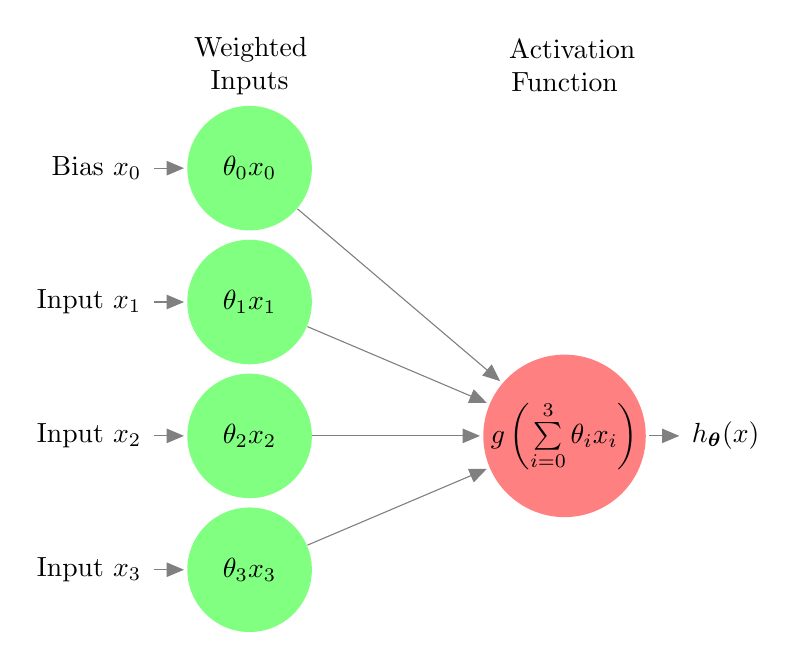
\begin{tikzpicture}[shorten >=1pt,->,draw=black!50, node distance=2.5cm]
    \tikzstyle{every pin edge}=[<-,shorten <=1pt]
    \tikzstyle{neuron}=[circle,fill=black!25,minimum size=45pt,inner sep=0pt]
    \tikzstyle{input neuron}=[neuron, fill=green!50];
    \tikzstyle{output neuron}=[neuron, fill=red!50];
    \tikzstyle{hidden neuron}=[neuron, fill=blue!50];
    \tikzstyle{annot} = [text width=4em, text centered]

    % Draw the input layer nodes
 %   \foreach \name / \y in {0,...,3}
    % This is the same as writing \foreach \name / \y in {1/1,2/2,3/3,4/4}
        \node[input neuron, pin=left:Bias $x_0$] (I-0) at (0,-0) {$\theta_0 x_0$};
	\foreach \name / \y in {1,...,3}
    % This is the same as writing \foreach \name / \y in {1/1,2/2,3/3,4/4}
        \node[input neuron, pin=left:Input $x_{\y}$] (I-\name) at (0,-1.7*\y) {$\theta_{\y}x_\y$};
    % Draw the hidden layer nodes
    %\foreach \name / \y in {1,...,5}
     %   \path[yshift=0.5cm]
      %      node[hidden neuron] (H-\name) at (\layersep,-\y cm) {};

    % Draw the output layer node
    \node[output neuron,pin={[pin edge={->}]right:$h_{\bm{\theta}}(x)$}, right of=I-2, node distance=4cm] (O) {$g\left(\sum\limits^3_{i=0}\theta_ix_i\right)$};

    % Connect every node in the input layer with every node in the
    % hidden layer.
   % \foreach \source in {1,...,4}
    %    \foreach \dest in {1,...,5}
     %       \path (I-\source) edge (H-\dest);

    % Connect every node in the hidden layer with the output layer
    \foreach \source in {0,...,3}
        \path (I-\source) edge (O);

    % Annotate the layers
%    \node[annot,above of=H-1, node distance=1cm] (hl) {Hidden layer};
    \node[annot,above of=I-0, node distance=1.3cm](il) {Weighted Inputs};
    \node[annot,right of=il, node distance=4cm] {Activation Function};
\end{tikzpicture}
\caption{\small Example structure of an individual node function with 3 inputs, labelled as $\bm{x}=[x_0\quad x_1\quad x_2\quad x_3]^\top$, with $x_0$ corresponding to the bias node. The weights are denoted as $\bm{\theta}=[\theta_0\quad \theta_1\quad \theta_2\quad \theta_3]$.}
\label{fig:2.1}
\end{figure}
\newpage
\section{Activation Functions}\label{sec:2.3}
Some common activation functions \citep{DeepLearning} are:
\begin{itemize}
\item The rectified linear unit (ReLU): 
\begin{gather*}
g: \R\rightarrow [0,\infty)\\ 
g(x)=\max\{0,x\},
\end{gather*}
\item The sigmoid or logistic activation function:
\begin{gather*}
g: \R\rightarrow (0,1)\\
g(x)=(1+\exp(-x))^{-1},
\end{gather*}
\item The hyperbolic tangent function:
\begin{gather*}
g:\R\rightarrow (-1,1)\\
g(x)=\tanh(x),
\end{gather*}
\item The linear activation function:
\begin{gather*}
g:\R\rightarrow \R\\
g(x)=x.
\end{gather*}
\end{itemize}
Their plots are shown in \autoref{fig:2.2}.
\begin{figure}[h]
\resizebox{\textwidth}{!}{
\begin{tikzpicture}
\begin{axis}[name=ReLU, xlabel=$x$, ylabel=$g(x)$, ymin=-0.5, ymax=2, xmin=-2, xmax=2, legend pos = north west]
\addplot [domain=-2:2, samples=100]{max(0,x)};
\addlegendentry{ReLU}
\end{axis}
\begin{axis}[name=Sigmoid, at=(ReLU.right of south east), anchor = left of south west, xlabel=$x$, ylabel=$g(x)$, ymin=-0.5, ymax=1.5, xmin=-2, xmax=2, legend pos = north west]
\addplot [domain=-2:2, samples=100]{1/(1+exp(-x))};
\addplot [dotted, domain=-2:2, samples=100]{1};
\addplot [dotted, domain=-2:2, samples=100]{0};
\addlegendentry{Sigmoid}
\end{axis}
\begin{axis}[name=Linear, at=(Sigmoid.below south west), anchor = above north west, xlabel=$x$, ylabel=$g(x)$, ymin=-2, ymax=2, xmin=-2, xmax=2, legend pos = north west]
\addplot [domain=-2:2, samples=100]{x};
\addlegendentry{Linear}
\end{axis}
\begin{axis}[name=Tanh, at=(Linear.left of south west), anchor = right of south east, xlabel=$x$, ylabel=$g(x)$, ymin=-1.5, ymax=1.5, xmin=-2, xmax=2, legend pos = north west]
\addplot [domain=-2:2, samples=100]{tanh(x)};
\addplot [dotted, domain=-2:2, samples=100]{1};
\addplot [dotted, domain=-2:2, samples=100]{-1};
\addlegendentry{Tanh}
\end{axis}
\end{tikzpicture}
}
\caption{Activation Function Plots}
\label{fig:2.2}
\end{figure}\\
The choice of activation function is dependent on several factors:
\begin{itemize}
\item The node's location in the network,
\item Desired node output range,
\item Continuous differentiability is ideal for gradient-based optimization methods \citep{snyman},
\item Monotonic activation functions ensure that the error is convex \citep{wu},
\item In cases where the output range is restricted, the level of input signal required for the activation function output to be asymptotically close to its limit.
\end{itemize}

For example, if the node's output is the estimate of a probability (ranging in $(0,1)$), then the sigmoid function would be used \citep{cybenko}. In addition to its ideal output range, the sigmoid function is continuously differentiable and requires significant input to output a value asymptotically close to $0$ or $1$. This allows the probability to be estimated with greater precision than with an activation function that approaches its limits very quickly, such as the hyperbolic tangent function.

On the other hand, if the node's output is the network's estimation of a non-negative quantity, such as price or time, then the ReLU activation function may be ideal, as its output ranges in $[0,\infty)$, and its linearity makes the overall node operation similar to linear regression.

We now describe the overall neural network structure, as the choice of activation function is dependent on the node's relative location on the network.
\section{Neural Network Structure}\label{sec:2.4}
A typical neural network is made up of layers of interconnected nodes \citep{neuralstat}. The first layer, called the input layer, does not have an activation function or weights, rather it simply acts as an input interface for the network. The outputs from the nodes can only be sent to nodes in succeeding layers, with the exception of the final output layer; it's result is simply the output of the network. The layers of nodes between the input and output layer are called the \textit{hidden} layers, as their outputs are generally not interpreted by the user. Hidden layers can have an arbitrary number of nodes, whilst the nodes in the input and output layers are restricted to the desired number of inputs and outputs of the model. Example 2.4.1 explains the arithmetic operations within a neural network, and is illustrated in \autoref{fig:2.3}.

The choice of activation function for a node in a neural network is typically dependent on its layer. The input layer can be described as having a linear activation function, as it has no activation function. Rectified linear units are the default choice for the hidden layers for their many advantages \citep{DeepLearning}:
\begin{itemize}
\item Sparsity: since negative ReLU inputs result in a zero output, not all of the units are ``active" (non-zero output) during the network's runtime. Sparsity is preferred in neural networks as it reduces overfitting and makes the model more robust to insignificant changes in input \citep{sparse}.
\item Faster computation: the $\max\{0,x\}$ function is computed much faster than the exponential or hyperbolic tangent function.
\item Better gradient propagation: weight training in a neural network (discussed in Sections \ref{sec:2.6} and \ref{sec:2.7}) involves `back-propagating' a loss value through the network, which calculates the partial derivatives of the loss function with respect to the weights. The weights subsequently receive a change proportional to their partial derivative. Back-propagation uses the chain rule, so activation functions such as sigmoid or tanh that have a low gradient near their asymptotes may experience the `vanishing gradient problem', in which the calculated partial derivatives become increasingly small as the loss value propagates through the network \citep{kolen}. This causes the front layers to train very slowly. The ReLU activation function does not experience this issue as it its gradient is either linear or $0$ \citep{sparse}.
\end{itemize}

The types of activation functions used in the output layer have been explained in \autoref{sec:2.3}.
\begin{figure}[h]
\centering
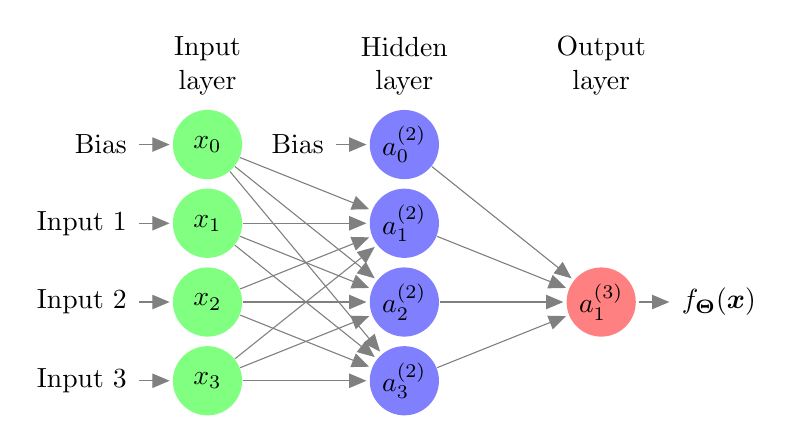
\begin{tikzpicture}[shorten >=1pt,->,draw=black!50, node distance=2.5cm]
    \tikzstyle{every pin edge}=[<-,shorten <=1pt]
    \tikzstyle{neuron}=[circle,fill=black!25,minimum size=25pt,inner sep=0pt]
    \tikzstyle{input neuron}=[neuron, fill=green!50];
    \tikzstyle{output neuron}=[neuron, fill=red!50];
    \tikzstyle{hidden neuron}=[neuron, fill=blue!50];
    \tikzstyle{annot} = [text width=4em, text centered]
    
	\node[input neuron, pin=left:Bias] (I-0) at (0,0) {$x_0$};
    % Draw the input layer nodes
    \foreach \name / \y in {1,...,3}
    % This is the same as writing \foreach \name / \y in {1/1,2/2,3/3,4/4}
        \node[input neuron, pin=left:Input \y] (I-\name) at (0,-\y) {$x_\y$};

 \path[yshift=0cm]
            node[hidden neuron, pin=left:Bias] (H-0) at (2.5cm,0) {$a^{(2)}_0$};
    % Draw the hidden layer nodes
    \foreach \name / \y in {1,...,3}
        \path[yshift=0cm]
            node[hidden neuron] (H-\name) at (2.5cm,-\y) {$a^{(2)}_\y$};

    % Draw the output layer node
	\path[yshift=1cm]    
    node[output neuron,pin={[pin edge={->}]right:$f_{\bm{\Theta}}(\bm{x})$}, right of=H-2] (O) {$a_1^{(3)}$};

    % Connect every node in the input layer with every node in the
    % hidden layer.
    \foreach \source in {0,...,3}
        \foreach \dest in {1,...,3}
            \path (I-\source) edge (H-\dest);

    % Connect every node in the hidden layer with the output layer
    \foreach \source in {0,...,3}
        \path (H-\source) edge (O);

    % Annotate the layers
    \node[annot,above of=H-0, node distance=1cm] (hl) {Hidden layer};
    \node[annot,left of=hl] {Input layer};
    \node[annot,right of=hl] {Output layer};
\end{tikzpicture}
\caption{\small Example of a neural network structure with 3 external inputs, 1 hidden layer (with 3 nodes), 1 bias node per non-output layer and 1 output node. The variable inside each node denotes it's output as calculated in \autoref{sec:2.2}: the output of node $i$ in layer $j$ is denoted as $a_i^{(j)}$. $\bm{\Theta}$ denotes the weights of the network.}
\label{fig:2.3}
\end{figure}
\begin{example}
In this example, we follow \autoref{fig:2.3}, describing a neural network with 3 inputs, 1 hidden layer with 3 nodes and 1 output node. We denote the activation function as $g$, the output of node $i$ in layer $j$ as $a^{(j)}_i$, and the matrix of weights from layer $j$ to $j+1$ as $\Theta^{(j)}$. We also use the subscript $\Theta^{(j)}_{m,n}$ where $m$ is the row of the matrix corresponding to the node $m$ in layer $j+1$, and $n$ is the column of the matrix relating to node $n$ in layer $j$.

Denoting the weights outputting to unit $i$ in layer $j+1$ as $\bm{\theta}^{(j)}_i$, we have the following relation between the node weights (as described in \autoref{sec:2.2}) and these weight matrices: $\bm{\theta}^{(j)}_i = \left[\Theta_{i,0}^{(j)}\quad \Theta_{i,1}^{(j)}\cdots \Theta_{i,k}^{(j)}\right]^\top$, where $k+1$ is the number of inputs.

Individually, the outputs in the hidden nodes and the output node are:
\[x_0=1,\qquad a_0^{(2)}=1,\]
\[a_1^{(2)}=g\left(\Theta^{(1)}_{1,0}x_0+\Theta^{(1)}_{1,1}x_1+\Theta^{(1)}_{1,2}x_2+\Theta^{(1)}_{1,3}x_3\right)=g\left((\bm{\theta}^{(1)}_1)^\top\bm{x}\right),\]
\[a_2^{(2)}=g\left(\Theta^{(1)}_{2,0}x_0+\Theta^{(1)}_{2,1}x_1+\Theta^{(1)}_{2,2}x_2+\Theta^{(1)}_{2,3}x_3\right)=g\left((\bm{\theta}^{(1)}_2)^\top\bm{x}\right),\]
\[a_3^{(2)}=g\left(\Theta^{(1)}_{3,0}x_0+\Theta^{(1)}_{3,1}x_1+\Theta^{(1)}_{3,2}x_2+\Theta^{(1)}_{3,3}x_3\right)=g\left((\bm{\theta}^{(1)}_3)^\top\bm{x}\right),\]
\[f_\Theta(\bm{x})=a_1^{(3)}=g\left(\Theta^{(2)}_{1,0}a_0^{(2)}+\Theta^{(2)}_{1,1}a_1^{(2)}+\Theta^{(2)}_{1,2}a_2^{(2)}+\Theta^{(2)}_{1,3}a_3^{(2)}\right)=g\left((\bm{\theta}^{(2)}_1)^\top\bm{a}^{(2)}\right),\]
where $\bm{a}^{(2)}=\left[a_0^{(2)}\quad a_1^{(2)}\quad a_2^{(2)}\quad a_3^{(3)}\right]^\top$.
%An even simpler notation is:
%\[a_0^{(2)}=1\]
%\[[a_1^{(2)}\quad a_2^{(2)}\quad a_3^{(2)}]=g((\Theta^{(1)})^\top\bm{x})\]
%\[f_{\bm{\Theta}} (\bm{x})=\bm{a}^{(3)}=g((\Theta^{(2)})^\top\bm{a}^{(2)}).\]
\end{example}
\section{Weight Initialization}\label{sec:2.5}
Proper initialization of the weights $\bm{\Theta}$ is ideal to improve network training (discussed in Sections \ref{sec:2.6} and \ref{sec:2.7}), as if the weights are too small, then the nodal outputs will continually decrease through the layers and become very small, resulting in a significant loss value which requires many iterations of training to fix. A similar scenario occurs when the initial weights are too high \citep{bishop}. In this section we discuss \textit{Xavier Initialization} \citep{xavier}, a common initialization method used in deep learning which aims to keep the signal variance constant throughout the network. To derive this algorithm, first consider a single node with $n+1$ inputs, and let $z$ denote the weighted sum of the inputs $\bm{\theta}^\top\bm{x}$ before it is passed through the activation function. This is written as
\[z=\theta_0+\sum^n_{i=1}\theta_ix_i.\]
Here, $\theta_0$ is constant with respect to the external input, so $\Var(\theta_0)=0$. Now without any prior knowledge of the inputs and weights, we arbitrarily assume that they are independent and have 0 mean. We can then find the variance of the other terms by using the formula for the product of independent variables \citep{goodman}:
\begin{align*}
\Var(\theta_ix_i)&=\E[x_i]^2\Var(\theta_i)+\E[\theta_i]^2\Var(x_i)+\Var(\theta_i)\Var(x_i)\\
&=\Var(\theta_i)\Var(x_i).
\end{align*}
Assuming that the weights and inputs are also identically distributed, we have
\[\Var(z)=n\Var(\theta_i)\Var(x_i).\]
Since we want constant variance of the signals throughout the network, we set $\Var(z)=\Var(x_i)$ and the result follows:
\[\Var(\theta_i)=\frac1n.\]
However, this result only considers forward propagation of the signal. A variation of this result accounts for back propagation by averaging the number of input and output nodes:
\[\Var(\theta_i)=\frac{2}{n_{in}+n_{out}}.\]
Thus, to enforce constant signal variance throughout the network, the Xavier initialization of weights samples from a density, typically Gaussian, with $0$ mean and $\frac{2}{n_{in}+n_{out}}$ variance:
\[\theta_i\sim \mathcal{N}\left(0,\frac{2}{n_{in}+n_{out}}\right).\]
\section{Optimization}\label{sec:2.6}
The goal of optimizing the network is to train the weights of the network such that a loss function, which we will denote as $L$, is minimized. A common loss function is the squared error between the batch of network outputs and the actual results:
\[L(\Theta)=\frac12 (\bm{y}-\bm{f}_\Theta(\bm{x}))^\top(\bm{y}-\bm{f}_\Theta(\bm{x})).\]
The $\frac12$ factor is included to eliminate the factor of 2 in the derivative, simplifying the derivations. The derivative is multiplied by an arbitrary training rate during optimization so there is no significant impact of including that factor \citep{DeepLearning}.

\textit{Back-propagation} (\autoref{sec:2.7}) is used to calculate the partial derivative of the loss function with respect to each individual weight. These partial derivatives are used in the gradient-based optimization of the weights. There are many variations of neural network optimization algorithms, but they are mostly based off \textit{gradient descent}, which we will cover in this section \citep{optimneural}.
\begin{definition}
At point $\bm{x}^{(n)}$, $\bm{s}^{(n)}$ is a \textit{descent direction} if $\nabla f\left(\bm{x}^{(n)}\right)^\top \bm{s}^{(n)}<0$.
\end{definition}
Gradient descent \citep{optim} is an algorithm used to find the minimizer $\bm{x}^*$ of a function $f$ by iterating on an arbitrary point $\bm{x}^{(n)}$, taking steps proportional to a descent direction $\bm{s}^{(n)}$:
\[\bm{x}^{(n+1)}=\bm{x}^{(n)}+\alpha \bm{s}^{(n)},\qquad \alpha>0.\]
%\begin{figure}
%\centering
%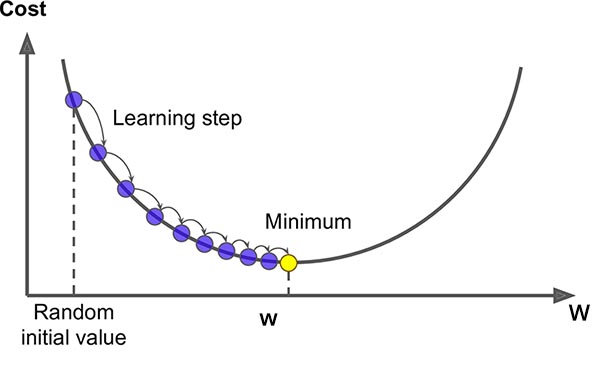
\includegraphics[scale=2]{gradientdescent.jpg}
%\caption{Gradient Descent}
%\end{figure}
\begin{proposition} \citep{beck} If $\bm{s}^{(n)}$ is a descent direction for $x^{(n)}$, then for sufficiently small $\alpha>0$,
\[f\left(\bm{x}^{(n)}+\alpha \bm{s}^{(n)}\right)<f\left(\bm{x}^{(n)}\right).\]
\begin{proof}
A proof of this proposition can be found in \autoref{app:A.1}.
\end{proof}
\end{proposition}
A common choice of descent direction is the negative of the gradient, that is, $-\nabla f\left(\bm{x}^{(n)}\right)$. It is clearly a descent direction as 
\begin{align*}
\nabla f(\bm{x}^{(n)})^\top\nabla f\left(\bm{x}^{(n)}\right)&=-\|\nabla f\left(\bm{x}^{(n)}\right)\|^2\\
&<0,
\end{align*} where $\|\cdot\|$ denotes the Euclidean norm.

By nature, gradient descent is guaranteed to converge to a local minimum, which is problematic if the function has local minima which differ from the global minima. This is not an issue in this thesis, as each loss functions that we use is convex, so therefore any local minima are also global minima. Those interested in global optimization can refer to ``Deterministic Global Optimization" by \citet{floudas}.

Typically, the entire batch of data is used in each iteration to calculate the loss function and gradient values required for gradient descent. This method of \textit{batch gradient descent} is very slow for large datasets. \textit{Stochastic gradient descent} is defined by the use of only one observation per iteration, so the latent randomness associated with each observation effectively leads to noise added to each step, but the optimization is much faster. In practice, a compromise between stochastic and batch gradient descent is typically used; \textit{mini-batch gradient descent} involves using several observations per iteration, reducing the gradient variance \citep{batch, optimneural}. The size of the batch depends on the size and nature of the data set. For small data sets, the batch would typically be the entire data set as this would be computationally feasible. On the other hand, online datasets are stochastic in nature and generally very large, so a small batch size is ideal \citep{bengio}.

Gradient descent convergence can be improved by using an \textit{adaptive learning rate}, defined by the adjustment of the value of $\alpha$ over the iterations. This is because a low learning rate leads to slow convergence, whilst a high learning rate can cause the algorithm to oscillate around the minima \citep{optimneural}.

In this thesis, we use the \textit{Adam algorithm}, which incorporates mini-batch gradient descent and an adaptive training rate to form an effective optimization algorithm that is commonly applied to neural networks. It uses the first and second moments of the gradient decay rate to adapt the weight training rate. More details can be found in ``Adam: A Method for Stochastic Optimization" by \citet{adam}.
\section{Back-Propagation}\label{sec:2.7}
In the back-propagation algorithm, the goal is to find the partial derivative of the loss function with respect to the individual weights \[\frac{\partial}{\partial\Theta_{m,n}^{(j)}}L(\Theta),\]
so that gradient descent can be performed to optimize the weights \citep{backprop}. For each training sample $\left(\bm{x}^{(I)},\bm{y}^{(I)}\right)$, $I=1,\dots,N$, the input signal is propagated forward throughout the network to calculate $\bm{a}^{(j)}$ for $j=2,\dots,J$, where $J$ is the total number of layers. The difference $\bm{\delta}^{(J)}$ between the network output and the ideal result is calculated with 
\[\bm{\delta}^{(J)}=\bm{a}^{(J)}-\bm{y}^{(I)},\] 
and this error is propagated backwards through the network to find $\bm{\delta}^{(J-1)},\dots,\bm{\delta}^{(2)}$ by using the formula 
\[\bm{\delta}^{(j)}=\left(\left(\Theta^{(j)}\right)^\top \bm{\delta}^{(j+1)}\right).*g'\left(\Theta^{(j)^\top} \bm{a}^{(j)}\right),\] 
where $.*$ denotes element-wise multiplication and $g'$ is the derivative of the activation function. Note that $\bm{\delta}^{(1)}$ does not need to be calculated as the input layer is not weighted. \\
The errors for each layer are multiplied by each of the preceding layer's activation outputs to form the estimated partial derivative for the training sample. This result is added to an accumulator matrix, so that the average partial derivative from all the training samples can be computed:
\[\Delta^{(j)}_{m,n}\coloneqq\Delta^{(j)}_{m,n}+a_n^{(j)}\delta_m^{(j+1)}.\]
Finally, we divide the accumulator matrix entries by the number of training samples to find the average partial derivative of the cost function with respect to the weights:
\[\frac{\partial}{\partial \Theta^{(j)}_{m,n}}L(\Theta)=\frac1N \Delta_{m,n}^{(j)}.\]
Pseudocode for back-propagation is shown in \autoref{app:B.1}.\\

\chapter{Variational Inference}\label{ch3}
In this chapter, we explain \textit{variational inference}, a method in Bayesian statistics that uses a specific functional form to approximate posterior densities. These are called `variational densities', from the use of variational calculus to derive certain expressions. We first describe the Bayesian framework and problems associated with computational intractability. We then explain, with examples, two types of variational inference: mean-field variational inference and amortized inference. Finally, the chapter concludes with a description of issues that arise when one or more of the involved are implicit densities, that is, samples can be readily drawn from them but the density function is difficult to numerically evaluate.
\section{Context}\label{sec:3.1}
A fundamental problem in Bayesian statistics is to evaluate, or estimate posterior densities, so that inference on unknown parameters can be performed \citep{gelman}. Consider the set of latent and known variables $\bm{z}=(z_1,\dots,z_M)\in \R^M$ and $\bm{x}=(x_1,\dots,x_N)\in \R^N$, respectively, with joint density $p(\bm{z},\bm{x})$. The posterior density $p(\bm{z}|\bm{x})$ is the density of the latent parameters $\bm{z}$ conditioned on the known variables $\bm{x}$. Applying Bayes' theorem, it can be written as
\begin{equation*}
p(\bm{z}|\bm{x})=\frac{p(\bm{z},\bm{x})}{p(\bm{x})}= \frac{p(\bm{z})p(\bm{x}|\bm{z})}{\int_\R p(\bm{z},\bm{x})\, {\rm d}\bm{z}},
\end{equation*}
where
\begin{itemize}
\item $p(\bm{z})$ is the prior density: the initial density of $\bm{z}$ before the data $\bm{x}$ is observed. This can be initialized to represent our subjective beliefs, or it can be an uninformative prior that implies objectivity.
\item $p(\bm{x}|\bm{z})$ is the likelihood: the density of data $\bm{x}$ conditioned on latent $\bm{z}$.
\item $p(\bm{x})=\int_\mathcal{z}p(\bm{z},\bm{x})d\bm{z}$ is the marginal likelihood, or the evidence: the density of the data averaged across all possible parameter values.
\end{itemize}
In simple cases, the posterior can typically be calculated algebraically by using the proportionality $p(\bm{z}|\bm{x})\propto p(\bm{z})p(\bm{x|z})$ and normalising over the constant $p(\bm{x})$. As the model increases in complexity, the calculations required can become increasingly difficult, so
% the evidence integral $p(\bm{x})=\int_\mathbcal{z}p(\bm{z},\bm{x})d\bm{z}$ is computationally intractable, then we are unable to evaluate the posterior density. 
traditional Markov Chain Monte Carlo (MCMC) methods overcome this obstacle by sampling from a Markov chain that converges to the stationary density $p(\bm{z}|\bm{x})$. However, these methods tend to have slow convergence for large datasets or high dimensional data. When faced with these issues or when desiring a faster computation, one may instead apply variational inference, an alternative approach to density estimation. Variational inference can be much faster than MCMC as it replaces sampling with optimization, but it is known to underestimate the true posterior variance \citep{blei}.

\section{The KL Divergence}\label{sec:3.2}
We first define the $f$-\textit{divergence}: a measure of how much two probability densities differ.
\begin{definition}\label{def:3.2.1}
The $f$-divergence of continuous probability density $q(x)$ from $p(x)$ is
\[D_f(p(x)\|q(x))=\mathbb{E}_{p(x)}\left[f\left(\frac{q(x)}{p(x)}\right)\right],\]
where $f$ is a convex function such that $f(1)=0$.
\end{definition}
Setting $f(x)=-\log x$ leads to the derivation of the KL (Kullback-Leibler) divergence \citep{KL}, a commonly used $f$-divergence in variational inference \citep{blei}.
\begin{definition}
The KL divergence is the expected logarithmic difference between two densities $p(x)$ and $q(x)$ with respect to $p(x)$:
\begin{equation*}
KL(p(x)\|q(x))=\int_{-\infty}^\infty p(x)\log \left(\frac{p(x)}{q(x)}\right)\, {\rm d}x=\mathbb{E}_{p(x)}\left[\log\left(\frac{p(x)}{q(x)}\right)\right].
\end{equation*}
\end{definition}
\begin{remark}
The KL divergence is not symmetric:
\begin{equation*}
KL(p(x)||q(x))\neq KL(q(x)||p(x))\text{ for }p(x)\neq q(x).
\end{equation*}
\end{remark}
In variational inference, $KL(p(x)\|q(x))$ is known as the \textit{forward KL divergence}, whilst $KL(q(x)\|p(x))$ is the \textit{reverse KL divergence}.
\begin{lemma}
The reverse KL divergence is formulated when $f(x)=x\log x$ in an $f$-divergence.
\begin{proof}
Proof of this lemma can be found in \autoref{app:swag}.
\end{proof}
\end{lemma}
Note that the forward and reverse KL divergences mainly differ in the density that is used to take the expectation.
\begin{lemma}\label{3.2.5}
The KL divergence is non-negative, and it is equal to zero if and only if $p(x)$ and $q(x)$ are equivalent:
\begin{equation*}
KL(p(x)||q(x))\geq 0.
\end{equation*}
\begin{proof}
Proof of this lemma can be found in \autoref{app:asdf}.
\end{proof}
\end{lemma}
\section{Introduction to Variational Inference}\label{sec:3.3}
Variational inference approximates the true posterior density $p(\bm{z}|\bm{x})$ with a different density $q(\bm{z})$, taken from a tractable family of approximate densities $\mathcal{Q}$, and then minimizes the $f$-divergence between the two densities in an optimization problem \citep{blei}:
\begin{equation}\label{eqn:3.3.1}
q^*(\bm{z})=\argmin_{q(\bm{z})\in \mathcal{Q}}\left\lbrace D_f(q(\bm{z})\|p(\bm{z}|\bm{x}))\right\rbrace.
\end{equation}
This produces an analytic approximation to the posterior density. The most common $f$-divergence used in variational inference is the reverse KL divergence, used instead of the forward KL divergence as we are unable to sample from our true posterior $p(\bm{z}|\bm{x})$. Equation (\ref{eqn:3.3.1}) can therefore be written as
\begin{equation}\label{eqn:3.3.2}
q^*(\bm{z})=\argmin_{q(\bm{z})\in \mathcal{Q}}\left\lbrace KL(q(\bm{z})\|p(\bm{z}|\bm{x}))\right\rbrace.
\end{equation}
From Lemma \ref{3.2.5}, it can be deduced that $KL(q(\bm{z})\|p(\bm{z}|\bm{x}))$ attains a minimal value of $0$ when $q(\bm{z})$ and $p(\bm{z}|\bm{x})$ are equivalent.\\
We cannot evaluate the reverse KL divergence term in Equation (\ref{eqn:3.3.2}) directly as $p(\bm{z}|\bm{x})$ is unknown. Instead, we apply Bayes' law to the equation and rearrange the terms to formulate a tractable expression that can be optimized.
\section{Derivation of the ELBO}\label{sec:3.4}
In this section, we formulate the \textit{evidence lower bound} ($ELBO$) of our posterior inference problem. Maximization of this term is equivalent to solving Equation (\ref{eqn:3.3.2}). We begin by applying Bayes' law to the problem and expanding the terms:
\begin{align*}
q^*(\bm{z})&=\argmin_{q(\bm{z})\in \mathcal{Q}}\left\lbrace KL(q(\bm{z})\|p(\bm{z}|\bm{x}))\right\rbrace\\
&= \argmin_{q(\bm{z})\in \mathcal{Q}} \left\lbrace\mathbb{E}_{q(\bm{z})}[\log q(\bm{z})-\log p(\bm{z}|\bm{x})]\right\rbrace\\
&= \argmin_{q(\bm{z})\in \mathcal{Q}} \left\lbrace\mathbb{E}_{q(\bm{z})}\left[\log q(\bm{z})-\log\frac{p(\bm{x}|\bm{z})p(\bm{z})}{p(\bm{x})}\right]\right\rbrace\\
&= \argmin_{q(\bm{z})\in \mathcal{Q}} \left\lbrace\mathbb{E}_{q(\bm{z})}[\log q(\bm{z})-\log p(\bm{x}|\bm{z})-\log p(\bm{z})]+\log p(\bm{x})\right\rbrace.
\end{align*}
Note that in the last line $\mathbb{E}_{q(\bm{z})}[\log p(\bm{x})]=\log p(\bm{x})$ as $p(\bm{x})$ is independent of $q(\bm{z})$. Also note that we cannot evaluate this expression due to the intractability of $p(\bm{x})$, so we rearrange the KL divergence expression as follows:
\begin{align}
KL(q(\bm{z})\|p(\bm{z}|\bm{x}))&=\mathbb{E}_{q(\bm{z})}[\log q(\bm{z})-\log p(\bm{x}|\bm{z})-\log p(\bm{z})]+\log p(\bm{x}) \nonumber \\
\log p(\bm{x})-KL(q(\bm{z})\|p(\bm{z}|\bm{x}))&=-\mathbb{E}_{q(\bm{z})}[\log q(\bm{z})-\log p(\bm{x}|\bm{z})-\log p(\bm{z})]\nonumber \\
&=\mathbb{E}_{q(\bm{z})}[\log p(\bm{x}|\bm{z})]-\mathbb{E}_{q(\bm{z})}[\log q(\bm{z})-\log p(\bm{z})]\nonumber \\
&=\mathbb{E}_{q(\bm{z})}[\log p(\bm{x}|\bm{z})]-KL(q(\bm{z})\|p(\bm{z}))\nonumber\\
\log p(\bm{x})&\geq \mathbb{E}_{q(\bm{z})}[\log p(\bm{x}|\bm{z})]-KL(q(\bm{z})\|p(\bm{z})).
\end{align}
We refer to $\mathbb{E}_{q(\bm{z})}[\log p(\bm{x}|\bm{z})]-KL(q(\bm{z})\|p(\bm{z}))$ as $ELBO(q)$, as it is the lower bound of the evidence density. Our minimization problem in Equation (\ref{eqn:3.3.2}) is now equivalent to maximizing $ELBO(q)$, so it can be written as:
\begin{align}
q^*(\bm{z})&=\argmin_{q(\bm{z})\in \mathcal{Q}}\left\lbrace KL(q(\bm{z})\|p(\bm{z}|\bm{x}))\right\rbrace\nonumber\\
&= \argmax_{q(\bm{z})\in \mathcal{Q}} \left\lbrace ELBO(q)\right\rbrace\nonumber\\
&= \argmax_{q(\bm{z})\in \mathcal{Q}} \left\lbrace\mathbb{E}_{q(\bm{z})}[\log p(\bm{x}|\bm{z})]-KL(q(\bm{z})\|p(\bm{z}))\right\rbrace.\nonumber
\end{align}
%We remark that Expression (3.4.3) attains a maximum at the marginal likelihood of the dataset $\log p(\bm{x})$, hence we may use the value of $ELBO(q)$ to construct a model selection criterion \citep{pattern}. However, this criterion may not be reliable as it is a lower bound.
\section{Mean-Field Variational Family}\label{sec:3.5}
The family of variational densities $\mathcal{Q}$ is typically a `\textit{mean-field variational family}', in which the density $q(\bm{z})$ factorizes over the latent variables $\{z_i\}^M_{i=1}$, each with an individual set of parameters $\{\phi_i\}^M_{i=1}$ \citep{blei}:
\begin{equation*}
q(\bm{z})=\prod^M_{i=1}q_{\phi_i}(z_i).
\end{equation*}
The individual factors $q_{\phi_i}(z_i)$ can take any form, but they are typically assumed to be independent, simplifying derivations but reducing the estimation accuracy when the latent variables in the true posterior density $p(\bm{z}|\bm{x})$ exhibit dependence. Fixing the forms of the individual factors, we want to choose the parameters $\phi_i$ such that $ELBO(q)$ is maximized. A derivation of the optimal factor $q_{\phi_i}^*(z_i)$ can be found in \autoref{app:mfvi}, and leads to the following equation:
\[q^*_{\phi_i}(z_i)\propto \exp\left(\mathbb{E}_{\bm{z}_{-i}}[\log p(z_i|\bm{z}_{-i},\bm{x})]\right).\]
This expression can be used in an \textit{expectation-maximization algorithm}, in which the factor $q^*_{\phi_i}(z_i)$ is evaluated and iterated from $i=1,\dots, M$ until $ELBO(q)$ converges. (We can say convergence occurs when there is little variation in $ELBO(q)$ over the iterations.) This particular algorithm is called \textit{coordinate ascent variational inference} (CAVI); pseudocode can be found in \autoref{alg:6} in \autoref{app:B.2}. \autoref{app:C} exemplifies mean-field variational inference, closely following the ``Bayesian Mixture of Gaussians" example from ``Variational Inference: A Review for Statisticians" by \citet{blei}.
\section{Amortized Inference}
Now consider the case where we have $K$ data points, each with dimensionality $N$. We denote the set of data points as $\bm{X}=\left[\bm{x}^{(1)},\dots,\bm{x}^{(K)}\right]^\top$, where $\bm{x}^{(i)}=(x^{(i)}_1,\dots,x^{(i)}_N)\in \R^N$, $i=1,\dots,K$. One disadvantage of mean field variational inference is that a specific set of variational parameters needs to be derived and optimized for each of these data points. This is computationally expensive for large datasets, and is because the parametrization of the posterior $p(\bm{z}|\bm{x})$ changes as the data point $\bm{x}$ changes. We therefore denote our set of latent variables as $\bm{Z}=(\bm{z}^{(1)},\dots,\bm{z}^{(K)})^\top$, where $\bm{z}^{(i)}=(z^{(i)}_1,\dots,z^{(i)}_M)\in \R^M$, $i=1,\dots,K$. In mean-field variational inference, each latent variable $z_j^{(i)}$ has its own individual set of parameters $\phi_j^{(i)}$, so overall there are $M\times N$ sets of parameters.

Amortized inference resolves this issue by using a single, constant set of parameters for all data points, adding the data point itself as an input to the variational density \citep{ADVVI}. This practice is defined as \textit{amortizing} the density. Our variational density therefore conditions on the observation, taking the form
\[q_\phi(\bm{z}|\bm{x}).\]
Figures \ref{fig:3.1} and \ref{fig:3.2} highlight the difference between mean-field and amortized variational inference.\\
\begin{figure}[h]
  \centering
  \tikz{ %
    \node[latent] (phi) {$\bm{\phi}^{(i)}$} ; %
    \node[latent, right=of phi] (z) {$\bm{z}^{(i)}$} ; %
    \plate[inner sep=0.25cm, xshift=-0.12cm, yshift=0.12cm] {plate1} {(phi) (z)} {$i\in \{1:K\}$}; %
    \edge {phi} {z} ; %
   
  }
   \caption{\small This DAG represents Mean-Field Variational Inference. For each of the $K$ datasets, a set of parameter sets $\bm{\phi^{(i)}}$ corresponding to each latent variable point $\bm{z}^{(i)}$ has to be found. $\bm{\phi}^{(i)}$ is $M$-dimensional, so there is a total of $M\times K$ sets of parameters.}
   \label{fig:3.1}
\end{figure}
\begin{figure}[h]
\centering
  \tikz{ %
    \node[obs] (x) {$\bm{x}^{(i)}$} ; %
    \node[latent, above=of x] (phi) {$\bm{\phi}$} ; %
    \node[latent, right=of x] (z) {$\bm{z}^{(i)}$} ; %
    \plate[inner sep=0.25cm, xshift=-0.12cm, yshift=0.12cm] {plate1} {(x) (z)} {$i\in \{1:K\}$}; %
    \edge {phi} {z} ; %
    \edge {x} {z} ;
    
  }
  \caption{\small This DAG represents Amortized Variational Inference. Here, there is only one set of variational parameters $\bm{\phi}$, and each data point $\bm{x}^{(i)}$ is used as an input in the variational posterior $q_{\bm{\phi}}(\bm{z}|\bm{x})$ to find $\bm{z}^{(i)}$.}
  \label{fig:3.2}
\end{figure}\\
A very complex model is required for such a structure, so it typically takes the form of a neural network with $\bm{x}$ as an input. This method is often used in deep learning due to the significant amount of data required to train such a network.

Recall that $p(\bm{x})$ represents the `true' density of the data. This is typically unavailable, so we instead represent it with the density of a sample dataset, which we denote as $q^*(\bm{x})$. Since our variational posterior conditions on data point $\bm{x}$, we now aim to minimize the expectation of the KL divergence with respect to $q^*(\bm{x})$:
\begin{align*}
\phi &=\argmin_\phi \left\lbrace\mathbb{E}_{q^*(\bm{x})}\left[KL(q_\phi(\bm{z}|\bm{x})\|p(\bm{z}|\bm{x}))\right]\right\rbrace\\
&= \argmin_\phi \left\lbrace\mathbb{E}_{q^*(\bm{x})q_\phi (\bm{z}|\bm{x})}\left[\log q_\phi(\bm{z}|\bm{x})-\log p(\bm{z}|\bm{x})\right]\right\rbrace\\
&=\argmin_\phi\left\lbrace\mathbb{E}_{q^*(\bm{x})q_\phi (\bm{z}|\bm{x})}\left[\log q_\phi(\bm{z}|\bm{x})-\log \frac{p(\bm{x}|\bm{z})p(\bm{z})}{p(\bm{x})}\right]\right\rbrace\\
&=\argmin_\phi\left\lbrace\mathbb{E}_{q^*(\bm{x})q_\phi (\bm{z}|\bm{x})}\left[\log q_\phi(\bm{z}|\bm{x})-\log p(\bm{x}|\bm{z})-\log p(\bm{z})\right]+\log p(\bm{x})\right\rbrace.
\end{align*} 
Again, we cannot evaluate this expression as $p(\bm{x})$ is intractable, so we rearrange the terms to form the evidence lower bound, which we aim to maximize to minimize the KL divergence.
\begin{align*}
ELBO(q)&=\mathbb{E}_{q^*(\bm{x})}[\log p(\bm{x})-KL(q_\phi(\bm{z}|\bm{x})\|p(\bm{z}|\bm{x}))]\\
&=-\mathbb{E}_{q^*(\bm{x})q_\phi(\bm{z}|\bm{x})}\left[\log q_\phi(\bm{z}|\bm{x})-\log p(\bm{x}|\bm{z})-\log p(\bm{z})\right]\\
&=\mathbb{E}_{q^*(\bm{x})q_\phi(\bm{z}|\bm{x})}\left[\log p(\bm{x}|\bm{z})+\log p(\bm{z})-\log q_\phi(\bm{z}|\bm{x})\right]\\
&=\mathbb{E}_{q^*(\bm{x})}\left[\E_{q_\phi(\bm{z}|\bm{x})}[\log p(\bm{x}|\bm{z})]-KL(q_\phi(\bm{z}|\bm{x})\|p(\bm{z}))\right].
\end{align*}
We take the negative of $ELBO(q)$ to form the \textit{negative evidence lower bound} $NELBO(q)$:
\begin{equation*}
NELBO(q)\coloneqq\mathbb{E}_{q^*(\bm{x})}\left[-\E_{q_\phi(\bm{z}|\bm{x})}[\log p(\bm{x}|\bm{z})]+KL(q_\phi(\bm{z}|\bm{x})\|p(\bm{z}))\right],
\end{equation*}
which we aim to minimize with respect to the variational posterior weights $\phi$:
\begin{equation}
\min_\phi \lbrace NELBO(q)\rbrace.
\end{equation}
Since $\phi$ represents the parameters of a neural network, it is unnecessary to find the specific weight values during back-propagation: we are more interested in training the network to optimality, achieved by minimizing the objective function. Hence, it is more appropriate to write the optimization problem with $\min$ than with $\argmin$.

In deep learning, the likelihood term $p(\bm{x}|\bm{z})$ is often represented as a neural network parametrized by $\theta$: $p_\theta(\bm{x}|\bm{z})$. This network is optimized alongside the variational density, in a formation known as the variational autoencoder.
\section{Example: Variational Autoencoder}\label{sec:3.7}
A \textit{variational autoencoder} (\autoref{fig:3.3}) is a model consisting of two simultaneously trained neural networks: an encoder representing the posterior density $q_\phi(\bm{z}|\bm{x})$ that ``compresses" a data point $\bm{x}=(x_1,\dots,x_N)$ into a lower dimensional latent representation $\bm{z}$, and a decoder representing the likelihood density $p_\theta(\bm{x}|\bm{z})$ that ``reconstructs" the data point from the latent variable \citep{kingma}. Typically, the prior $p(\bm{z})$ is simply a standard multivariate normal density with dimensionality equal to that of the latent variable point $\bm{z}=(z_1,\dots,z_M)$: $\mathcal{N}(0,I_{M\times M})$. The autoencoder has two main purposes: lower-dimensional representation learning of data, and data generation. We now reiterate our optimization problem in Equation (3.6.1), this time including the optimization of the decoder parameters $\theta$:
\begin{equation}
\min_{\phi,\theta} \left\lbrace\mathbb{E}_{q^*(\bm{x})}\left[-\E_{q_\phi(\bm{z}|\bm{x})}[\log p_\theta(\bm{x}|\bm{z})]+KL(q_\phi(\bm{z}|\bm{x})\|p(\bm{z}))\right]\right\rbrace.
\end{equation}
The first term is the negative likelihood, analogous to the error between the original and reconstructed data, which we aim to minimize. The KL divergence between the variational posterior and the prior density acts as a regularizer term. Without it, the encoder would learn to segregate distinct data types in separate regions of the Euclidean plane, which runs contrary to the randomness of a probability density. Due to this regularizer term, we can generate new data $\bm{x}$ by sampling $\bm{z}\sim p(\bm{z})$ and feeding it through the decoder \citep{vae}. This is illustrated in \autoref{fig:3.4}.

In our current formulation, we are trying to represent the variational posterior density with a deterministic neural network, so for any arbitrary fixed data point $\bm{x}$, the value of the encoder's latent output $\bm{z}$ is always the same. The solution is to add a noise density to the model to make it probabilistic. Instead of the encoder outputting the posterior sample $\bm{z}$ directly, we configure it to output a mean vector $\bm{\mu}=(\mu_1,\mu_2,\cdots,\mu_M)^\top$ and variance vector $\bm{\sigma}^2=(\sigma^2_1,\sigma^2_2,\cdots, \sigma^2_M)^\top$, each with dimensions equal to that of latent variable $\bm{z}$. We then define $\bm{z}$ as an output from a multivariate normal density with means and variances as specified by the encoder output:
\[q_\phi(\bm{z}|\bm{x})\sim \mathcal{N}(\bm{\mu},\bm{\sigma}^2I_{M\times M}).\]
Often in practice, this is achieved by sampling random standard normal noise $\bm{\varepsilon}$, multiplying it by the variance and adding the result to the mean:
\[\bm{\varepsilon}\sim \mathcal{N}(0,I_{M\times M}),\qquad \bm{z}=\bm{\mu}+\bm{\varepsilon}\cdot\bm{\sigma}^2.\]
A similar process of adding random noise is used for the decoder network representing the likelihood density $p_\theta(\bm{x}|\bm{z})$, but it's parametrization is chosen depending on the nature of the data. For example, a multivariate normal parametrization similar to our variational posterior can be used for most continuous data. For binary data, a sigmoid output layer is specified in the neural network and the likelihood is expressed as a Bernoulli density with probabilities given by the network output.
\begin{lemma}
Using the explicit form of the multivariate normal $q_\phi(\bm{z}|\bm{x})$ and $p(\bm{z})$ densities, the KL divergence term can be calculated through the equation:
\[KL(q_\phi(\bm{z}|\bm{x})\|p(\bm{z}))=\frac12 \sum_{i=1}^M\left(\sigma^2_i+\mu^2_i-\log(\sigma^2_i)-1\right).\]
\begin{proof}
Proof of this lemma can be found in \autoref{app:A.2}.
\end{proof}
\end{lemma}
We can evaluate and minimize $NELBO(q)$ in Equation (3.7.1) as we have an explicit parametrization of all of the terms.
\begin{figure}[h]
  \centering
  \tikz{ %
    \node[latent] (x) {$\bm{x}$} ; %
    \node[det, right=of x] (q) {$q_\phi(\bm{z}|\bm{x})$} ; %
    \node[latent, right=of q] (qout) {$\bm{\mu}, \bm{\sigma}^2$} ;
    \node [det, right=of qout] (para1) {$+,*$} ;
    \node [latent, above=of para1] (eps) {$\bm{\varepsilon}_1$} ;
    \node [latent, right=of para1] (z) {$\bm{z}$} ;
    \node [det, right=of z] (p) {$p_\theta(\bm{x}|\bm{z})$} ;
    \node [latent, right=of p] (pout) {$\tilde{\bm{x}}$} ;
    \node [latent, above=of p] (eps2) {$\bm{\varepsilon}_2$} ;
    \edge {x} {q} ; %
    \edge {q} {qout} ;
    \edge {qout} {para1} ;
    \edge {eps} {para1} ;
    \edge {para1} {z} ;
    \edge {z} {p} ;
    \edge {p} {pout} ;
    \edge[dashed] {eps2} {p} ;
  }
   \caption{\small A simple DAG representing a Variational Autoencoder. An arbitrary data point $\bm{x}$ is passed through the encoder $q_\phi(\bm{z}|\bm{x})$ to produce a mean vector $\bm{\mu}$ and a variance vector $\bm{\sigma}^2$. Random noise $\bm{\varepsilon}_1$ is sampled from $\mathcal{N}(0,I_{M\times M})$ and transformed to generate $\bm{z}$: $\bm{z}=\bm{\mu}+\bm{\varepsilon}\cdot \bm{\sigma}^2$. This latent variable $\bm{z}$ is passed through the decoder $p_\theta(\bm{x}|\bm{z})$ to reconstruct the data point as $\tilde{\bm{x}}$. Note that random noise $\bm{\varepsilon}_2$ is not a direct input into the decoder, rather it represents the noise density added to make the neural network probabilistic.}
   \label{fig:3.3}
\end{figure}
\begin{figure}[h]
  \centering
  \tikz{ %
    \node [latent] (z) {$\bm{z}$} ;
    \node [det, right=of z] (p) {$p_\theta(\bm{x}|\bm{z})$} ;
    \node [latent, right=of p] (pout) {$\tilde{\bm{x}}$} ;
    \node [latent, above=of p] (eps2) {$\bm{\varepsilon}_2$} ;
    \edge {z} {p} ;
    \edge {p} {pout} ;
    \edge[dashed] {eps2} {p} ;
  }
   \caption{\small To generate new data $\tilde{\bm{x}}$ similar to existing data $\bm{x}$, we sample latent variable $\bm{z}$ from the prior density $p(\bm{z})$ and pass it through the decoder $p_\theta(\bm{x}|\bm{z})$.}
   \label{fig:3.4}
\end{figure}
\section{Problems with Implicit Densities}\label{sec:3.8}
The above sections assume that the prior $p(\bm{z})$, likelihood ($p(\bm{x}|\bm{z})$ or $p_\theta(\bm{x}|\bm{z})$) and variational posterior $q_\phi(\bm{z}|\bm{x})$ have an explicit form. However, there are two main scenarios in which at least one of these densities is implicit, that is, the parametrization of their density is difficult to numerically evaluate but we are able to easily generate samples from them. This poses problems with optimization as the objective function becomes difficult to compute. 
\subsection{Implicit Prior and/or Variational Posterior}\label{sec:3.8.1}
In the first scenario, at least one of the prior $p(\bm{z})$ or variational posterior $q_\phi(\bm{z}|\bm{x})$ densities is \textit{implicit}, but the likelihood is known. An implicit prior is rare but may occur in posterior inference. The implicit variational posterior case occurs more often (in both posterior inference and data generation), and is detailed in ``Adversarial Variational Bayes" by \citet{mescheder}.

In amortized inference, the variational posterior sample $\bm{z}$ is typically sampled from an independent multivariate normal density with means and variances defined by the variational network. However, this representation lacks dependencies between the latent variables, and therefore fails to effectively model multi-modal or flexible densities. In his paper, Mescheder adds random noise $\bm{\varepsilon}\sim \pi(\bm{\varepsilon})$ as additional inputs to the variational network, training the network to directly output $\bm{z}$. $\pi(\bm{\varepsilon})$ is a typical noise density, such as $\mathcal{N}(0,I_{p\times p})$ where $p$ is the desired number of noise inputs. This added noise allows the probabilistic nature of a random density to be represented by a deterministic neural network. However, note that the neural network does not output the probability density $q_\phi(\bm{z}|\bm{x})$, rather it outputs a sample $\bm{z}\sim q_\phi(\bm{z}|\bm{x})$. Retaining the network parameters $\phi$, we denote the generator of posterior samples as $\mathcal{G}_\phi(\bm{\varepsilon};\bm{x})$. A diagram illustrating this is shown in \autoref{fig:3.5}.
\begin{figure}[h]
  \centering
  \tikz{ %
    \node[latent] (x) {$\bm{x}$} ; %
    \node[det, right=of x] (q) {$\mathcal{G}_\phi(\bm{\varepsilon}_1;\bm{x})$} ; %
    \node [latent, above=of q] (eps) {$\bm{\varepsilon}_1$} ;
    \node [latent, right=of q] (z) {$\bm{z}$} ;
    \node [det, right=of z] (p) {$p_\theta(\bm{x}|\bm{z})$} ;
    \node [latent, right=of p] (pout) {$\tilde{\bm{x}}$} ;
    \node [latent, above=of p] (eps2) {$\bm{\varepsilon}_2$} ;
    \edge {x} {q} ; %
    \edge {q} {z}
    \edge {eps} {q} ;
    \edge {z} {p} ;
    \edge {p} {pout} ;
    \edge[dashed] {eps2} {p} ;
  }
   \caption{\small This diagram depicts the ``Adversarial Variational Bayes" formulation of the variational autoencoder. Rather than transforming random noise $\varepsilon_1$ according to the mean vector $\bm{\mu}$ and variance vector $\bm{\sigma}$ output of the variational posterior $q_\phi(z|x)$, we add the noise to the encoder network $\mathcal{G}_\phi(\varepsilon_1;\bm{x})$ directly as an additional input. The likelihood density $p_\theta(\bm{x}|\bm{z})$ has the same explicit representation as in Figures \ref{fig:3.3} and \ref{fig:3.4}.}
   \label{fig:3.5}
\end{figure}

Due to the complex nature of the neural network, it is difficult to numerically compute the explicit form of $q_\phi(\bm{z}|\bm{x})$, but we are able to easily generate samples by feeding data and noise through the network, hence its implicit nature.

Now recall our optimization problem from Equation (3.7.1):
\[\min_{\phi,\theta} \left\lbrace\mathbb{E}_{q^*(\bm{x})}\left[-\E_{q_\phi(\bm{z}|\bm{x})}[\log p_\theta(\bm{x}|\bm{z})]+KL(q_\phi(\bm{z}|\bm{x})\|p(\bm{z}))\right]\right\rbrace.\]
When either the prior or variational posterior is implicit, this expression is difficult to evaluate as we are unable to calculate the KL divergence term:
\[KL(q_\phi(\bm{z}|\bm{x})\|p(\bm{z}))=\E_{q_\phi(\bm{z}|\bm{x})}\left[\log \frac{q_\phi(\bm{z}|\bm{x})}{p(\bm{z})}\right].\]
We therefore resort to \textit{density ratio estimation} techniques (\autoref{ch4}) to approximate $q_\phi(\bm{z}|\bm{x})/p(\bm{z})$, using only samples from the two densities.
\subsection{Implicit Likelihood}\label{sec:3.8.2}
When we apply amortized variational inference to an implicit likelihood density, the optimization problem is intractable even with density ratio estimation, as it is difficult to evaluate the likelihood term $-\E_{q_\phi(\bm{z}|\bm{x})}[\log p_\theta(\bm{x}|\bm{z})]$. This can occur in posterior inference or in some autoencoder variations where an implicit generative function $G(\bm{\varepsilon};\bm{x})$ is used to represent the likelihood density $p_\theta(\bm{x}|\bm{z})$ \citep{ali}. An example of the latter case is illustrated in \autoref{fig:3.6}.
\begin{figure}[h]
  \centering
  \tikz{ %
    \node[latent] (x) {$\bm{x}$} ; %
    \node[det, right=of x] (q) {$\mathcal{G}_\phi(\bm{\varepsilon}_1;\bm{x})$} ; %
    \node [latent, above=of q] (eps) {$\bm{\varepsilon}_1$} ;
    \node [latent, right=of q] (z) {$\bm{z}$} ;
    \node [det, right=of z] (p) {$G_\theta(\bm{\varepsilon}_2;\bm{x})$} ;
    \node [latent, right=of p] (pout) {$\tilde{\bm{x}}$} ;
    \node [latent, above=of p] (eps2) {$\bm{\varepsilon}_2$} ;
    \edge {x} {q} ; %
    \edge {q} {z}
    \edge {eps} {q} ;
    \edge {z} {p} ;
    \edge {p} {pout} ;
    \edge {eps2} {p} ;
  }
   \caption{\small This diagram depicts a variation of ``Adversarial Variational Bayes", in which random noise $\bm{\varepsilon}_2$ is additionally added to the input of the generator of likelihood density samples $G_\theta(\bm{\varepsilon}_2;\bm{x})$. The likelihood density $p_\theta(\bm{x}|\bm{z})$ is therefore implicit and consequently, its corresponding term in the optimization problem cannot be evaluated.}
   \label{fig:3.6}
\end{figure}

We rephrase the optimization problem, instead minimizing the reverse KL divergence between the two joint densities \citep{tran}: \[KL(q(\bm{z},\bm{x})\|p(\bm{z},\bm{x}))=\E_{q(\bm{z},\bm{x})}\left[\log\frac{q(\bm{z},\bm{x})}{p(\bm{z},\bm{x})}\right].\] We derive this by applying Bayes' theorem to the reverse KL divergence between the true and variational posterior densities, this time formulating the joint densities:
\begin{align*}
\mathbb{E}_{q^*(\bm{x})}\left[KL(q_\phi(\bm{z}|\bm{x})\|p_\theta (\bm{z}|\bm{x}))\right]&=\mathbb{E}_{q^*(\bm{x})q(\bm{z}|\bm{x})}\left[\log \frac{q(\bm{z}|\bm{x})p(\bm{x})}{p(\bm{x}|\bm{z})p(\bm{z})}\right]\\
&=\mathbb{E}_{q^*(\bm{x})q(\bm{z}|\bm{x})}\left[\log \frac{q(\bm{z}|\bm{x})q^*(\bm{x})}{p(\bm{x}|\bm{z})p(\bm{z})}\right]+\mathbb{E}_{q^*(\bm{x})}\left[\log \frac{p(\bm{x})}{q^*(\bm{x})}\right]\\
&= \mathbb{E}_{q^*(\bm{x})q(\bm{z}|\bm{x})}\left[\log \frac{q(\bm{z},\bm{x})}{p(\bm{z},\bm{x})}\right]-KL(q^*(\bm{x})\|p(\bm{x})).
\end{align*}
Recall that $p(\bm{x})$ is typically unavailable, so we are unable to evaluate $KL(q^*(\bm{x})\|p(\bm{x}))$ even with density ratio estimation techniques. Since it is constant, we add it to both sides of the equation, leading to the following expression for $NELBO(q)$:
\begin{align*}
NELBO(q) &= KL(q^*(\bm{x})\|p(\bm{x}))+\mathbb{E}_{q^*(\bm{x})}\left[KL(q_\phi(\bm{z}|\bm{x})\|p_\theta(\bm{z}|\bm{x}))\right]\\
&=\mathbb{E}_{q^*(\bm{x})q_\phi(\bm{z}|\bm{x})}\left[\log \frac{q(\bm{z},\bm{x})}{p(\bm{z},\bm{x})}\right].
\end{align*}
This expression attains a minimum at $KL(q^*(\bm{x})\|p(\bm{x}))$ when \[\mathbb{E}_{q^*(\bm{x})}\left[KL(q_\phi(\bm{z}|\bm{x})\|p_\theta(\bm{z}|\bm{x}))\right]=0,\] that is, the true and variational posteriors are equivalent with respect to the density of the data set. We therefore have the following lower bound:
\[\mathbb{E}_{q^*(\bm{x})q_\phi(\bm{z}|\bm{x})}\left[\log \frac{q(\bm{z},\bm{x})}{p(\bm{z},\bm{x})}\right]\geq KL(q^*(\bm{x})\|p(\bm{x})).\]
Our objective now is to minimize $NELBO(q)$ with respect to our variational parameters $\phi$:
\begin{equation}
\min_\phi \left\lbrace\mathbb{E}_{q^*(\bm{x})q_\phi(\bm{z}|\bm{x})}\left[\log \frac{q(\bm{z},\bm{x})}{p(\bm{z},\bm{x})}\right]\right\rbrace.
\end{equation}
Again, this term is approximated with density ratio estimation techniques. For consistency, we retain the notation of our variational posterior loss function as $NELBO(q)$. Note that the objective problem no longer has an explicit likelihood term, and can therefore be used with an implicit likelihood density. Since density ratio estimation only requires samples from the two densities, both the prior and variational posterior densities can also be implicit, hence the ``Adversarial Variational Bayes" representation (\autoref{fig:3.5}) of the variational network can be used.

In the autoencoder representation (\autoref{fig:3.6}), the forward KL divergence is additionally minimized with respect to the likelihood parameters \citep{tiao}:
\begin{equation}
\min_\theta \left\lbrace\mathbb{E}_{p(\bm{z})p_\theta(\bm{x}|\bm{z})}\left[\log \frac{p(\bm{z},\bm{x})}{q(\bm{z},\bm{x})}\right]\right\rbrace.
\end{equation}
In this scenario, separate density ratio estimators are typically used for Equations (3.8.1) and (3.8.2).
\chapter{Density Ratio Estimation}\label{ch4}
In this chapter, we derive two common methods of density ratio estimation used with implicit models \citep{sugiyama, mohamed}: \textit{class probability estimation} and \textit{divergence minimization}, applying them to the objective functions in both the implicit prior/posterior and implicit likelihood scenarios to formulate bi-level optimization problems. In this thesis, we follow the terminology in ``Variational Inference using Implicit Distributions" by \citet{huszar}, referring to the implicit prior/posterior objective as ``\textit{prior-contrastive}" and the implicit likelihood objective as ``\textit{joint-contrastive}".
\section{Class Probability Estimation}\label{sec:4.1}
\subsection{Derivation}\label{sec:4.1.1}
First, consider the probability density functions $p(u)$ and $q(u)$ defined on $U\subseteq \R^S$. We aim to estimate the density ratio $q(u)/p(u)$, given only samples from the two densities. In this thesis, we assume that for all $u\in U$, $p(u)>0$ and $q(u)>0$, avoiding the division of zero in density ratio estimation.

We take $m$ samples from $p(u)$: $U_p=\{u_1^{(p)},\dots,u_m^{(p)}\}$
and label them with $y=0$, then we take $n$ samples from $q(u)$: $U_q=\{u_1^{(q)},\dots, u_n^{(q)}\}$ and label them with $y=1$. Therefore, $p(u)=P(u|y=0)$ and $q(u)=P(u|y=1)$. By applying Bayes' theorem, we derive an expression for the density ratio:
\begin{align*}
\frac{q(u)}{p(u)}&= \frac{P(u|y=1)}{P(u|y=0)}\\
&= \left.\frac{P(y=1|u)P(u)}{P(y=1)}\middle/ \frac{P(y=0|u)P(u)}{P(y=0)}\right.\\
&= \frac{P(y=1|u)}{P(y=0|u)}\times \frac{P(y=0)}{P(y=1)}\\
&= \frac{P(y=1|u)}{P(y=0|u)}\times \frac{n}{m}.
\end{align*}
Often in practice, $m=n$, simplifying the density ratio to
\[\frac{q(u)}{p(u)}=\frac{P(y=1|u)}{P(y=0|u)},\]
which is the ratio of the probability that an arbitrary sample $u$ was taken from the density $q(u)$ to the probability that it was taken from $p(u)$. If we define a \textit{discriminator} function $D(u)\simeq P(y=1|u)$ that estimates these probabilities, then our density ratio can be expressed in terms of this function:
\[\frac{q(u)}{p(u)}\simeq \frac{D(u)}{1-D(u)}.\]
At optimality, the discriminator provides an exact estimate of the probability that the sample was taken from $q(u)$, so we have $D^*(u)=P(y=1|u)$ and therefore,
\[\frac{q(u)}{p(u)}=\frac{D^*(u)}{1-D^*(u)}.\]
The discriminator function typically takes the form of a neural network with parameters $\alpha$. It  can be trained by minimizing the \textit{Bernoulli loss} (the negative log-likelihood of the Bernoulli density), which we denote as $L_D$ \citep{sugiyama}:
\[L_D\coloneqq-\E_{q(u)}[\log D_\alpha(u)]-\E_{p(u)}[\log(1-D_\alpha(u))].\]
\begin{lemma}
The discriminator reaches optimality at $D^*_\alpha(u)=q(u)/(q(u)+p(u))$, minimizing its Bernoulli loss \citep{gan}.
\begin{proof}
Proof of this lemma can be found in \autoref{app:A.3}.
\end{proof}
\end{lemma}
\begin{remark}\label{rem:4.1.2}
$D^*_\alpha(u)$ is bound in $(0,1)$, so typically a sigmoid activation function is used for its output layer. Note that $D^*_\alpha (u)\neq 0$ and $D^*_\alpha(u)\neq 1$ as we have assumed $p(u)>0$ and $q(u)>0$ for all $u\in U$.
\end{remark}
\begin{remark}\label{rem:4.1.3}
When $q(u)$ and $p(u)$ are equivalent, that is, $q(u)=p(u)$, the discriminator cannot distinguish between samples from the two densities, outputting a probability of $\frac{1}{2}$: $D^*_\alpha(u)=\frac{1}{2}$. Substituting this value into the Bernoulli loss function, we obtain its minimal value when the two densities are equivalent and the discriminator is at its optimal parametrization: $L_{D^*}=\log 4$.
\end{remark}
In the context of amortized variational inference, the optimal discriminative loss can be used to check when the variational posterior has converged, that is, when the variational density $q_\phi(z|x)$ is equivalent to the true posterior density $p(z|x)$.
\subsection{Prior-Contrastive Algorithm}\label{sec:4.1.2}
We now turn to the prior-contrastive problem in Expression (3.6.1) of minimizing $NELBO(q)$
\begin{align}
\min_{\phi} \left\lbrace NELBO(q)\right\rbrace&=\min_{\phi}\left\lbrace\mathbb{E}_{q^*(x)}\left[-\E_{q_\phi(z|x)}[\log p(x|z)]+KL(q_\phi(z|x)\|p(z))\right]\right\rbrace\nonumber\\
&=\min_\phi \left\lbrace-\mathbb{E}_{q^*(x)q_\phi(z|x)}[\log p(x|z)]+\mathbb{E}_{q^*(x)q_\phi(z|x)}\left[\log \frac{q_\phi(z|x)}{p(z)}\right]\right\rbrace,
% &=\min_\phi \left\lbrace-\mathbb{E}_{q^*(x)\pi(\varepsilon)}[\log p(x|\mathcal{G}_\phi(\varepsilon;x)]+\mathbb{E}_{q^*(x)\pi(\varepsilon)}\left[\log \frac{q_\phi(\mathcal{G}_\phi(\varepsilon;x)|x)}{p(\mathcal{G}_\phi(\varepsilon;x))}\right]\right\rbrace,
\end{align}
which requires us to find the density ratio between $q_\phi(z|x)$ and $p(z)$.\\
If we label samples from $q_\phi(z|x)$ with $y=1$ and samples from $p(z)$ with $y=0$, we have the density ratio expression:
\[\frac{q_\phi(z|x)}{p(z)}=\frac{P(y=1|z)}{P(y=0|z)}.\]
We now define a discriminator function with parameters $\alpha$ that calculates the probability that an arbitrary sample $z$ belongs to the variational posterior $q_\phi(z|x)$. Since the posterior changes depending on the observation $x$, we also amortize the discriminator by taking an additional input from the dataset density $q^*(x)$, as opposed to training multiple discriminators for each observation:
\[D_\alpha(z,x)\simeq P(y=1|z).\]
As a binary classifier, this function can be trained by inputting an equal number of samples from both densities and minimizing its Bernoulli loss:
\begin{equation}
\min_\alpha \left\lbrace-\mathbb{E}_{q^*(x)q_\phi(z|x)}[\log D_\alpha(z,x)]-\mathbb{E}_{q^*(x)p_\theta(z)}[\log (1-D_\alpha(z,x))]\right\rbrace.
\end{equation}
We can now express the expected log ratio in terms of the probability that a posterior sample is correctly classified by the discriminator:
\begin{align*}
\mathbb{E}_{q^*(x)q_\phi(z|x)}\left[\log \frac{q_\phi(z|x)}{p(z)}\right]&=\mathbb{E}_{q^*(x)q_\phi(z|x)}\left[\log \frac{P(y=1|z)}{P(y=0|z)}\right]\\
&\simeq \mathbb{E}_{q^*(x)q_\phi(z|x)}\left[\log \frac{D_\alpha(z,x)}{1-D_\alpha(z,x)}\right].
\end{align*}
Our $NELBO$ optimization objective in Expression (4.1.1) can now be written as:
\begin{equation}
\min_\phi \left\lbrace-\mathbb{E}_{q^*(x)q_\phi(z|x)}[\log p(x|z)]+\mathbb{E}_{q^*(x)q_\phi(z|x)}\left[\log \frac{D_\alpha(z,x)}{1-D_\alpha(z,x)}\right]\right\rbrace.
\end{equation}
Recall from Remark \ref{rem:4.1.2} that a sigmoid activation function is typically used for the discriminator's output layer, so theoretically, the discriminator should never output its asymptotic limits of $0$ or $1$. However, numbers arbitrarily close to these limits may underflow or overflow to them when computationally stored in a floating point representation. Thus, when implementing this algorithm, we introduce a small constant $c>0$ to the numerator and denominator of the estimated density ratio:
\[\min_\phi \left\lbrace-\mathbb{E}_{q^*(x)q_\phi(z|x)}[\log p(x|z)]+\mathbb{E}_{q^*(x)q_\phi(z|x)}\left[\log \frac{D_\alpha(z,x)+c}{1-D_\alpha(z,x)-c}\right]\right\rbrace.\]

Since our variational posterior density is represented as a generative neural network function, our optimization objectives in Expressions (4.1.2) and (4.1.3) become:
\begin{align}
\min_\alpha \left\lbrace-\mathbb{E}_{q^*(x)\pi(\varepsilon)}[\log D_\alpha(\mathcal{G}_\phi(\varepsilon;x),x)-\mathbb{E}_{p_\theta(z)q^*(x)}[\log (1-D_\alpha(z,x))]\right\rbrace,\\
\min_\phi \left\lbrace-\mathbb{E}_{q^*(x)\pi (\varepsilon)}[\log p(x|\mathcal{G}_\phi(\varepsilon;x))]+\mathbb{E}_{q^*(x)\pi(\varepsilon)}\left[\log \frac{D_\alpha(\mathcal{G}_\phi(\varepsilon;x),x)}{1-D_\alpha(\mathcal{G}_\phi(\varepsilon;x),x)}\right]\right\rbrace.
\end{align}
In practice, the algorithm cycles between taking multiple gradient descent steps of the discriminative loss in Expression (4.1.4) with respect to $\alpha$ (with the generator parameters fixed) and taking one gradient descent step of $NELBO(q)$, as stated in Expression (4.1.5) (with the discriminator parameters fixed). If we apply this algorithm to an autoencoder, we would additionally parametrize the likelihood with $\theta$ and optimize $NELBO(q)$ with respect to those parameters.

Also note that from Equation (3.4.1) that $NELBO(q)$ has a lower bound of $-\log p(x)$, which is unknown. It is therefore inadequate to assess convergence using the value of $NELBO(q)$, so we would additionally check that the discriminative loss is arbitrarily close to $\log 4$, using Remark \ref{rem:4.1.3}.\\
Pseudocode for this algorithm is shown in \autoref{alg:1}.
\begin{algorithm}[t]
\SetKw{update}{update}
\caption{Prior-Contrastive Class Probability Estimation}
\KwIn{Dataset density $q^*(x)$, (implicit) prior $p(z)$, likelihood $p(x|z)$, noise density $\pi(\varepsilon)$}
\KwResult{Optimized posterior generator $\mathcal{G}_\phi(\varepsilon;x)$}
\BlankLine
\For{$j=1$ \KwTo $J$}{
	\For{$k=1$ \KwTo $K$}{
		Sample $\{\varepsilon^{(i,k)}\}^B_{i=1}\sim \pi(\varepsilon)$\;
		Sample $\{x^{(i,k)}\}^B_{i=1}\sim q^*(x)$\;
		\ForEach{$\varepsilon^{(i,k)}, x^{(i,k)}$}{
			Sample $z^{(i,k)}_q=\mathcal{G}(\varepsilon^{(i,k)};x^{(i,k)})$\;
		}
		Sample $\{z^{(i,k)}_p\}^B_{i=1}\sim p(z)$\;
		\update{$\alpha$ by optimization step on}{
			$\min_\alpha \left\lbrace\frac{1}{B}\sum^B_{i=1}\left[-\log D_\alpha\left(z_q^{(i,k)},x^{(i,k)}\right)-\log \left(1-D_\alpha\left(z_p^{(i,k)},x^{(i,k)}\right)\right)\right]\right\rbrace$\;
			%$\min_\alpha -\mathbb{E}_{q^*(x)\pi(\varepsilon)}[\log D_\alpha(\mathcal{G}_\phi(\varepsilon;x),x)]-\mathbb{E}_{p(z)q^*(x)}[\log (1-D_\alpha(z,x))]$\;
		}	
	}
	Sample $\{\varepsilon^{(i)}\}^B_{i=1}\sim \pi(\varepsilon)$\;
	Sample $\{x^{(i)}\}^B_{i=1}\sim q^*(x)$\;
	\ForEach{$\varepsilon^{(i)}, x^{(i)}$}{
			Sample $z^{(i)}_q=\mathcal{G}(\varepsilon^{(i)};x^{(i)})$\;
		}
	\update{$\phi$ by optimization step on}{
		$\min_\phi \left\lbrace\frac{1}{B}\sum^B_{i=1}\left[-\log p\left(x^{(i)}|z_q^{(i)}\right)+\log \frac{D_\alpha\left(z_q^{(i)},x^{(i)}\right)}{1-D_\alpha\left(z_q^{(i)},x^{(i)}\right)}\right]\right\rbrace$\;
	}
}
\label{alg:1}
\end{algorithm}
\subsection{Joint-Contrastive Algorithm}\label{sec:4.1.3}
We now restate from Expression (3.8.1) our optimization objective when the likelihood density is implicit:
\[\min_\phi \left\lbrace\mathbb{E}_{q^*(x)q_\phi(z|x)}\left[\log \frac{q(z,x)}{p(z,x)}\right]\right\rbrace,\]
or
\[\min_\phi \left\lbrace\mathbb{E}_{q^*(x)q_\phi(z|x)}\left[\log \frac{q_\phi(z|x)q^*(x)}{p(x|z)p(z)}\right]\right\rbrace.\]
Similar to the prior-contrastive case, we can label samples from $q(z,x)$ with $y=1$ and samples from $p(z,x)$ with $y=0$, leading to the density ratio expression:
\[\frac{q(z,x)}{p(z,x)}=\frac{P(y=1|z,x)}{P(y=0|z,x)}.\]
Again, we use a discriminator neural network $D_\alpha(z,x)\simeq P(y=1|z,x)$ to estimate the probability that samples $(z,x)$ came from the joint variational density $q(z,x)$. Using this discriminator function, our density ratio expression becomes:
\[\frac{q(z,x)}{p(z,x)}\simeq\frac{D_\alpha(z,x)}{1-D_\alpha(z,x)}.\]
The class probability algorithm again cycles between Bernoulli loss minimization of the discriminator:
\begin{equation}
\min_\alpha \left\lbrace-\mathbb{E}_{q^*(x)q_\phi(z|x)}[\log D_\alpha(z,x)]-\mathbb{E}_{p(z)p(x|z)}[\log (1-D_\alpha(z,x))]\right\rbrace
\end{equation}
and optimization of the variational posterior:
\begin{equation}
\min_\phi \left\lbrace\mathbb{E}_{q^*(x)q_\phi(z|x)}\left[\log\frac{D_\alpha(z,x)}{1-D_\alpha(z,x)}\right]\right\rbrace.
\end{equation}
Using the posterior generator parametrization $\mathcal{G}_\phi (\varepsilon;x)$, the optimization objectives in Expressions (4.1.6) and (4.1.7) become:
\[\min_\alpha \left\lbrace-\mathbb{E}_{q^*(x)\pi(\varepsilon)}[\log D_\alpha(\mathcal{G}_\phi(\varepsilon;x), x)]-\mathbb{E}_{p(z)p(x|z)}[\log (1-D_\alpha(z,x))]\right\rbrace\]
\[\min_\phi \left\lbrace\mathbb{E}_{q^*(x)\pi(\varepsilon)}\left[\log\frac{D_\alpha(\mathcal{G}_\phi(\varepsilon;x),x)}{1-D_\alpha(\mathcal{G}_\phi(\varepsilon;x),x)}\right]\right\rbrace.\]
Using Remark \ref{rem:4.1.3}, it can be seen that when $q(z,x)=p(z,x)$, the optimal generative loss is $0$. Pseudocode for the joint-contrastive class probability estimation algorithm is shown in \autoref{alg:2}.
\newpage
\begin{algorithm}
\SetKw{update}{update}
\caption{Joint-Contrastive Class Probability Estimation}
\KwIn{Dataset density $q^*(x)$, (implicit) prior $p(z)$, (implicit) likelihood $p(x|z)$, noise density $\pi(\varepsilon)$}
\KwResult{Optimized posterior generator $\mathcal{G}_\phi(\varepsilon;x)$}
\BlankLine
\For{$j=1$ \KwTo $J$}{
	\For{$k=1$ \KwTo $K$}{	
		Sample $\{\varepsilon^{(i,k)}\}^B_{i=1}\sim \pi(\varepsilon)$\;
		Sample $\{x^{(i,k)}_q\}^B_{i=1}\sim q^*(x)$\;
		\ForEach{$\varepsilon^{(i,k)},x^{(i,k)}$}{
			Sample $z^{(i,k)}_q=\mathcal{G}(\varepsilon^{(i,k)};x^{(i,k)}_q)$\;
		}
		Sample $\{z^{(i,k)}_p\}^B_{i=1}\sim p(z)$\;
		\ForEach{$z^{(i,k)}_p$}{
			Sample $x^{(i,k)}_p\sim p(x|z_p^{(i,k)})$\;
		}
		\update{$\alpha$ by optimization step on}{
		$\min_\alpha \left\lbrace\frac{1}{B}\sum^B_{i=1}\left[-\log D_\alpha\left(z_q^{(i,k)},x_q^{(i,k)}\right)-\log\left(1-D_\alpha\left(z_p^{(i,k)},x_p^{(i,k)}\right)\right)\right]\right\rbrace$\;
		%	$\min_\alpha -\mathbb{E}_{q^*(x)\pi(\varepsilon)}[\log D_\alpha(\mathcal{G}_\phi(\varepsilon;x), x)]-\mathbb{E}_{p(z)p(x|z)}[\log (1-D_\alpha(z,x))]$\;
		}
	}
	Sample $\{\varepsilon^{(i)}\}^B_{i=1}\sim \pi(\varepsilon)$\;
	Sample $\{x^{(i)}_q\}^B_{i=1}\sim q^*(x)$\;
	\ForEach{$\varepsilon^{(i)},x^{(i)}$}{
			Sample $z^{(i)}_q=\mathcal{G}(\varepsilon^{(i)};x^{(i)}_q)$\;
		}
	\update{$\phi$ by optimization step on\\}{
		$\enskip \left\lbrace\min_\phi \frac{1}{B}\sum^B_{i=1}\left[\log\frac{D_\alpha\left(z_q^{(i)},x_q^{(i)}\right)}{1-D_\alpha\left(z_q^{(i)},x_q^{(i)}\right)}\right]\right\rbrace$\;
	}
}
\label{alg:2}
\end{algorithm}
\section{Divergence Minimization}\label{sec:4.2}
In this section, we derive the divergence minimization density ratio estimation algorithm and apply it to our prior-contrastive and joint-contrastive optimization problems.
\subsection{Derivation}\label{sec:4.2.1}
We first define the \textit{convex conjugate}.
\begin{definition}
In $\R^S$, the convex conjugate $f^*(x^*)$ of a function $f(x)$ is:
\[f^*(x^*)\coloneqq \sup\left\lbrace\langle x^*,x\rangle-f(x)|x\in \R^S\right\rbrace,\]
where $\langle\cdot, \cdot\rangle$ denotes the standard inner product.
\end{definition}
Now recall from Definition \ref{def:3.2.1} that an $f$-divergence is defined by a convex function $f$ such that $f(1)=0$. A lower bound for the $f$-divergence in terms of a \textit{direct ratio estimator} $r(u)\simeq q(u)/p(u)$ can be found using the following theorem.
\begin{theorem}\label{4.2.1}  \citep{nguyen}
If $f$ is a convex function with derivative $f'$ and convex conjugate $f^*$, and $\mathcal{R}$ is a class of functions with codomains equal to the domain of $f'$, then we have the lower bound for the $f$-divergence between densities $p(u)$ and $q(u)$ in terms of a density ratio estimator $r(u)\in \mathcal{R}$:
\[D_f (p(u)\|q(u))\geq \sup_{r\in \mathcal{R}} \{\mathbb{E}_{q(u)}[f'(r(u))]-\mathbb{E}_{p(u)}[f^*(f'(r(u)))]\},\]
with equality when $r(u)=q(u)/p(u)$.
\begin{proof}
The proof of this theorem can be found in ``Estimating divergence functionals and the likelihood ratio by convex risk minimization" by \citet{nguyen}.
\end{proof}
\end{theorem}
The derivative and convex conjugate of $f(u)=u\log u$ are
\[f'(u)=1+\log u, \qquad f^*(u)=\exp(u-1),\]
so the convex conjugate of the derivative is simply $f^*(f'(u))=u$.\\
Using Theorem \ref{4.2.1}, we derive the following reverse KL divergence lower bound:
\begin{align}
D_{RKL}(p(x)\|q(x))&\coloneqq KL(q(u)\|p(u))\nonumber\\
&\geq \sup_{r\in \mathcal{R}}\{\mathbb{E}_{q(u)}[1+\log r(u)]-\mathbb{E}_{p(u)}[r(u)]\}.
\end{align}
Fixing the variational density $q(u)$, $KL(q(u)\|p(u))$ is constant, so recalling that the bound reaches equality when $r(u)=q(u)/p(u)$, we can represent the direct ratio estimator as a neural network parametrized by $\alpha$ and minimize the negative of Expression (4.2.1), which we define as $L_r$, with respect to $\alpha$:
\begin{equation}
L_r\coloneqq-\E_{q(u)}[\log r_\alpha(u)]+\E_{p(u)}[r_\alpha(u)].
\end{equation}
Note we have removed the $+1$ term as it is independent of $\alpha$.
\begin{lemma}
The direct ratio estimator reaches optimality at $r^*_\alpha(u)=q(u)/p(u)$, minimizing its ratio loss.
\begin{proof}
A proof using the first and second functional derivatives of the ratio loss can be found in \autoref{app:A.4}.
\end{proof}
\end{lemma}
\begin{remark}
$r_\alpha^*(u)$ is bound in $(0,\infty)$. Note that $r_\alpha^*(u)\neq 0$ as we have assumed that $p(u)>0$ and $q(u)>0$ for all $u\in U$.
\end{remark}
\begin{remark}\label{rem:4.2.4}
When the probability densities are equivalent, that is, $q(u)=p(u)$, the ratio estimator has a constant output of 1: $r^*_\alpha(u)=1$. This corresponds to a ratio estimator loss of $L_{r^*}=1$.
\end{remark}
Using Remark \ref{rem:4.2.4}, we can check for posterior convergence by observing when the ratio estimator loss becomes arbitrarily close to $1$.
\subsection{Prior-Contrastive Algorithm}\label{sec:4.2.2}
We begin by restating the optimization objective from Expression (4.1.1):
\[\min_\phi \left\lbrace-\mathbb{E}_{q^*(x)q_\phi(z|x)}[\log p(x|z)]+\mathbb{E}_{q^*(x)q_\phi(z|x)}\left[\log \frac{q_\phi(z|x)}{p(z)}\right]\right\rbrace.\]
Applying Theorem \ref{4.2.1}, we have the lower bound for the reverse KL divergence:
\[KL(q_\phi(z|x)\|p(z))\geq \sup_{\hat{r}\in \mathcal{R}}\{\mathbb{E}_{q_\phi(z|x)}[1+\log r(z)]-\mathbb{E}_{p(z)}[r(z)]\}.\]
Now we let our direct ratio estimator be a neural network parametrized by $\alpha$, and since $q_\phi(z|x)$ is dependent on the input $x\sim q^*(x)$, we add $x$ as an input and amortize the KL divergence across $q^*(x)$:
\[\mathbb{E}_{q^*(x)}\left[KL(q_\phi(z|x)\|p(z))\right]\geq \sup_\alpha \{\mathbb{E}_{q^*(x)q_\phi(z|x)}[1+\log r_\alpha(z,x)]-\mathbb{E}_{q^*(x)p(z)}[r_\alpha (z,x)]\}.\]
By taking the negative of this lower bound, we formulate the minimization problem for the direct ratio estimator:
\begin{equation}
\min_\alpha \left\lbrace-\E_{q^*(x)q_\phi(z|x)}[\log r_\alpha(z,x)]+\E_{q^*(x)p(z)}[r_\alpha (z,x)]\right\rbrace.
\end{equation}
Since $r_\alpha(z,x)\simeq q_\phi(z|x)/p(z)$, we write our $NELBO$ optimization problem in terms of the direct ratio estimator:
\begin{equation}
\min_\phi \left\lbrace-\mathbb{E}_{q^*(x)q_\phi(z|x)}\left[\log p(x|z)\right]+E_{q^*(x)q_\phi (z|x)}[\log r_\alpha(z,x)]\right\rbrace.
\end{equation}
Substituting the generator form of the posterior into Expressions (4.2.3) and (4.2.4), we have the bi-level optimization problem:
\[\min_\alpha \left\lbrace-\mathbb{E}_{q^*(x)\pi(\varepsilon)}[\log r_\alpha(\mathcal{G}_\phi(\varepsilon;x),x)]+\mathbb{E}_{q^*(x)p(z)}[r_\alpha(z,x)]\right\rbrace\]
\[\min_\phi \left\lbrace-\mathbb{E}_{q^*(x)\pi(\varepsilon)}\left[\log p(x|\mathcal{G}_\phi(\varepsilon;x)\right]+E_{q^*(x)\pi(\varepsilon)}[\log r_\alpha(\mathcal{G}(\varepsilon;x),x)]\right\rbrace.\]
Similar to class probability estimation, the algorithm involves cycling between multiple ratio estimator optimization steps and a single step of $NELBO$ minimization, as shown in \autoref{alg:3}.
\begin{algorithm}
\SetKw{update}{update}
\caption{Prior-Contrastive Divergence Minimization}
\KwIn{Dataset density $q^*(x)$, (implicit) prior $p(z)$, likelihood $p(x|z)$, noise density $\pi(\varepsilon)$}
\KwResult{Optimized posterior generator $\mathcal{G}_\phi(\varepsilon;x)$}
\BlankLine
\For{$j=1$ \KwTo $J$}{
	\For{$k=1$ \KwTo $K$}{
		Sample $\{\varepsilon^{(i,k)}\}^B_{i=1}\sim \pi(\varepsilon)$\;
		Sample $\{x^{(i,k)}\}^B_{i=1}\sim q^*(x)$\;
		\ForEach{$\varepsilon^{(i,k)}, x^{(i,k)}$}{
			Sample $z^{(i,k)}_q=\mathcal{G}(\varepsilon^{(i,k)};x^{(i,k)})$\;
		}
		Sample $\{z^{(i,k)}_p\}^B_{i=1}\sim p(z)$\;
		\update{$\alpha$ by optimization step on}{
			$\min_\alpha \left\lbrace\frac{1}{B}\sum^B_{i=1}\left[-\log \left(r_\alpha\left(z_q^{(i,k)},x^{(i,k)}\right)\right)+r_\alpha\left(z_p^{(i,k)},x^{(i,k)}\right)\right]\right\rbrace$\;
		}	
	}
	Sample $\{\varepsilon^{(i)}\}^B_{i=1}\sim \pi(\varepsilon)$\;
	Sample $\{x^{(i)}\}^B_{i=1}\sim q^*(x)$\;
	\ForEach{$\varepsilon^{(i)}, x^{(i)}$}{
			Sample $z^{(i)}_q=\mathcal{G}(\varepsilon^{(i)};x^{(i)})$\;
		}
	\update{$\phi$ by optimization step on}{
		$\min_\phi \left\lbrace\frac{1}{B}\sum^B_{i=1}\left[-\log p\left(x^{(i)}|z_q^{(i)}\right)+\log r_\alpha\left(z^{(i)}_q,x^{(i)}\right)\right]\right\rbrace$\;
	}
}
\label{alg:3}
\end{algorithm}
\subsection{Joint-Contrastive Algorithm}\label{sec:4.2.3}
First, we restate the problem from Expression (3.8.1) of minimizing the reverse KL divergence between the joint densities:
\[\min_\phi \left\lbrace\mathbb{E}_{q^*(x)q_\phi(z|x)}\left[\log \frac{q(z,x)}{p(z,x)}\right]\right\rbrace.\]
Applying Theorem \ref{4.2.1}, a lower bound for our KL divergence is
\[KL(q(z,x)\|p(z,x))\geq \sup_{r\in \mathcal{R}}\{\mathbb{E}_{q(z,x)}[1+\log r(z,x)]-\mathbb{E}_{p(z,x)}[r(z,x)]\}.\]
Note here we do not have to amortize our ratio estimator as the joint probability density already includes an input from the dataset. Again we set our ratio estimator to take the form of a neural network parametrized by $\alpha$:
\[r_\alpha(z,x)\simeq \frac{q(z,x)}{p(z,x)},\]
so that the lower bound becomes
\[KL(q(z,x)\|p(z,x))\geq \sup_{\alpha}\{\mathbb{E}_{q(z,x)}[1+\log r_\alpha(z,x)]-\mathbb{E}_{p(z,x)}[r_\alpha(z,x)]\}.\]
Again taking the negative of this lower bound, we formulate the following minimization problem for the direct ratio estimator:
\begin{equation}
\min_\alpha\left\lbrace-\E_{q^*(x)q_\phi(z|x)}[\log r_\alpha(z,x)]+\E_{p(z)p(x|z)}[r_\alpha(z,x)]\right\rbrace.
\end{equation}
The $NELBO$ minimization problem in terms of the direct ratio estimator is:
\begin{equation}
\min_\phi \left\lbrace\mathbb{E}_{q^*(x)q_\phi(z|x)}[\log r_\alpha(z,x)]\right\rbrace.
\end{equation}
Finally, we derive the bi-level optimization problem by writing the variational posterior term in Expressions (4.2.5) and (4.2.6) in terms of their generator form:
\[\min_\alpha \left\lbrace-\mathbb{E}_{q^*(x)\pi(\varepsilon)}[\log r_\alpha(\mathcal{G}(\varepsilon;x),x)]+\mathbb{E}_{p(z)p(x|z)}[r_\alpha(z,x)]\right\rbrace\]
\[\min_\phi \left\lbrace\mathbb{E}_{q^*(x)\pi(\varepsilon)}[\log r_\alpha(\mathcal{G}(\varepsilon;x),x)]\right\rbrace.\]
Again this process, shown in \autoref{alg:4}, involves cycling between multiple steps of optimizing the ratio estimator and taking a single optimization step of the $NELBO$.
\begin{algorithm}
\SetKw{update}{update}
\caption{Joint-Contrastive Divergence Minimization}
\KwIn{Dataset density $q^*(x)$, (implicit) prior $p(z)$, (implicit) likelihood $p(x|z)$, noise density $\pi(\varepsilon)$}
\KwResult{Optimized posterior generator $\mathcal{G}_\phi(\varepsilon;x)$}
\BlankLine
\For{$j=1$ \KwTo $J$}{
	\For{$k=1$ \KwTo $K$}{	
		Sample $\{\varepsilon^{(i,k)}\}^B_{i=1}\sim \pi(\varepsilon)$\;
		Sample $\{x^{(i,k)}_q\}^B_{i=1}\sim q^*(x)$\;
		\ForEach{$\varepsilon^{(i,k)},x^{(i,k)}_q$}{
			Sample $z^{(i,k)}_q=\mathcal{G}(\varepsilon^{(i,k)};x^{(i,k)}_q)$\;
		}
		Sample $\{z^{(i,k)}_p\}^B_{i=1}\sim p(z)$\;
		\ForEach{$z^{(i,k)}_p$}{
			Sample $x^{(i,k)}_p\sim p(x|z_p^{(i,k)})$\;
		}
		\update{$\alpha$ by optimization step on}{
			$\min_\alpha \left\lbrace\frac{1}{B}\sum^B_{i=1}\left[-\log \left(r_\alpha\left(z_q^{(i,k)},x^{(i,k)}_q\right)\right)+r_\alpha\left(z_p^{(i,k)},x^{(i,k)}_p\right)\right]\right\rbrace$\;
		}
	}
	Sample $\{\varepsilon^{(i)}\}^B_{i=1}\sim \pi(\varepsilon)$\;
	Sample $\{x^{(i)}_q\}^B_{i=1}\sim q^*(x)$\;
	\ForEach{$\varepsilon^{(i)},x^{(i)}_q$}{
			Sample $z^{(i)}_q=\mathcal{G}(\varepsilon^{(i)};x^{(i)}_q)$\;
		}
	\update{$\phi$ by optimization step on\\}{
		$\enskip\min_\phi \left\lbrace\frac{1}{B}\sum^B_{i=1}\left[\log r_\alpha\left(z_q^{(i)},x_q^{(i)}\right)\right]\right\rbrace$\;
	}
}
\label{alg:4}
\end{algorithm}
\subsection{Alternative Derivation of Class Probability Estimation}\label{sec:4.2.4}
If we apply the function $f(u)=u\log u-(u+1)\log (u+1)$ to Theorem \ref{4.2.1}, the resulting bi-level optimization problem is equivalent to that of class probability estimation \citep{tiao}. Before deriving the corresponding $f$-divergence, we define the \textit{Jenson-Shannon} divergence which will be used in the expression.
\begin{definition}
The Jensen-Shannon divergence is a symmetric metric used to measure the discrepancy between two probability densities \citep{JS}:
\[JS(p(u)\|q(u))=\frac12 KL(p(u)\|m(u))+\frac12 KL(q(u)\|m(u)),\]
where $m(u)=(q(u)+p(u))/2$.
\end{definition}
We denote this $f$-divergence as $D_{GAN}$ after the \textit{generative adversarial network} models which typically use the class probability estimation optimization problem \citep{gan}.
\begin{align*}
D_{GAN}(p(u)\|q(u))&= \E_{p(u)}\left[\frac{q(u)}{p(u)}\log \left(\frac{q(u)}{p(u)}\right)-\left(\frac{q(u)}{p(u)}+1 \right)\log\left(\frac{q(u)}{p(u)}+1\right)\right]\\
&= \int_U q(u)\log\left(\frac{q(u)}{p(u)}\right)-(q(u)+p(u))\log\left(\frac{q(u)+p(u)}{p(u)}\right)\,{\rm d}u\\
&= \int_U q(u)(\log q(u)-\log p(u))-(q(u)+p(u))\log(q(u)+p(u))\\
&\qquad +(q(u)+p(u))\log p(u)\enskip \,{\rm d}u\\
&= \int_U q(u)\log\left(\frac{q(u)}{q(u)+p(u)}\right)+p(u)\log \left(\frac{p(u)}{q(u)+p(u)}\right) \,{\rm d}u\\
&= \int_U p(u)\log \left(\frac{2p(u)}{q(u)+p(u)}\right)-p(u)\log 2+q(u)\log \left(\frac{2q(u)}{q(u)+p(u)}\right)\\
&\qquad -q(u)\log 2\enskip \,{\rm d}u\\
&= \int_U p(u)\left(\log \left(\frac{p(u)}{m(u)}\right)-\log 2\right)+q(u)\left(\log \left(\frac{q(u)}{m(u)}\right)-\log 2\right)\,{\rm d}u\\
&\text{ where }m(u)=\frac{q(u)+p(u)}{2}\\
&= \E_{p(u)} \left[\log \left(\frac{p(u)}{m(u)}\right)-\log 2\right]+\E_{q(u)}\left[\log\left(\frac{q(u)}{m(u)}\right)-\log 2\right]\\
&= KL(p(u)\|m(u))+KL(q(u)\|m(u))-\log 4\\
&= 2JS(p(u)\|q(u))-\log 4.
\end{align*}

Recall one of the conditions of $f$ to form an $f$-divergence is $f(1)=0$, but in this case, $f(1)=-\log 4$, hence the constant term in our GAN divergence.\\
The derivative and convex conjugate of $f(u)=u\log u-(u+1)\log (u+1)$ are
\[f'(u)=\log \left(\frac{u}{u+1}\right),\qquad f^*(u)=-\log (1-\exp u),\]
so the convex conjugate of the derivative is
\[f^*(f'(u))=\log (u+1).\]
Using Theorem \ref{4.2.1}, we derive the following lower bound for the Jensen-Shannon divergence:
\begin{align*}
D_{GAN}(p(u)\|q(u))&\coloneqq 2JS(p(u)\|q(u))-\log 4\\
&\geq \sup_{r\in \mathcal{R}}\left\lbrace\mathbb{E}_{q(u)}\left[\log \left(\frac{r(u)}{r(u)+1}\right)\right]-\mathbb{E}_{p(u)}[\log(r(u)+1)]\right\rbrace\\
&=\sup_{D\in \mathcal{R}}\{\E_{q(u)}[\log D(u)]+\E_{p(u)}[\log(1-D(u))]\},
\end{align*}
where $D(u)=r(u)/(r(u)+1)$. Maximization of the lower bound, equivalent to minimizing its negative, follows the optimization problem:
\[\min_\alpha \left\lbrace-\E_{q(u)}[\log D(u)]-\E_{p(u)}[\log (1-D(u))]\right\rbrace,\]
which is the discriminative loss of the class probability estimation approach. Equality of the bound is accomplished at the optimal function of
\begin{align*}
D^*(u)&=\frac{\frac{q(u)}{p(u)}}{\frac{q(u)}{p(u)}+1}\\
&=\frac{q(u)}{q(u)+p(u)},
\end{align*}
which is the optimal discriminator of class probability estimation. Thus, the density ratio in terms of this discriminator function is 
\[\frac{q(u)}{p(u)}\simeq \frac{D(u)}{1-D(u)}.\]
Therefore, our previous formulation of class probability estimation by minimizing the Bernoulli loss of a discriminator function is equivalent to maximizing the lower bound of the ``GAN" divergence between the two densities.
\chapter{Algorithm Generalization}\label{ch5}
In this chapter, we present the two density ratio estimation techniques in a comparable form, that is, in terms of the relevant $f$-divergence's lower bound as derived in \autoref{sec:4.2} using Theorem \ref{4.2.1}. From this, we generalize the density ratio algorithms to a selection of an $f$-divergence to formulate the lower bound and a parametrization of the density ratio estimator. We also suggest a third estimator parametrization: the \textit{direct log density ratio estimator} $T_\alpha(u)\simeq \log (q(u)/p(u))$. The derivations and comparisons of density ratio estimator loss functions using various $f$-divergences was explored in ``$f$-GAN: Training Generative Neural Samplers using Variational Divergence Minimization" by \citet{nowozin}, but this paper did not account for various parametrisations of the estimator. The formal generalization of density ratio estimation algorithms is the first contribution of this thesis.
\section{Introduction}\label{sec:5.1}
First, recall that within each of the prior-contrastive and joint-contrastive formulations, both class probability estimation and divergence minimization methods use the same $NELBO$ loss function to optimize the posterior weights. It is therefore evident that the only differences between the two density ratio estimation techniques are the estimator loss functions used. As shown in Subsections \ref{sec:4.2.1} and \ref{sec:4.2.4}, these estimator losses can be derived using \autoref{4.2.1}, hence the only differences between them lie within their $f$-divergence bound and the parametrization of the estimator. We reiterate these derivations below.

For divergence minimization, the following lower bound is achieved using the reverse KL divergence $D_{RKL}(p(u)\|q(u))=KL(q(u)\|p(u))$:
\begin{equation}\label{eq:5.1.1}
D_{RKL}(p(u)\|q(u))\geq \sup_{\alpha}\{\mathbb{E}_{q(u)}[1+\log r_\alpha(u)]-\mathbb{E}_{p(u)}[r_\alpha(u)]\},
\end{equation}
and class probability estimation follows the GAN divergence $D_{GAN}(p(u)\|q(u))=2JS(p(u)\|q(u))-\log 4$:
\begin{equation}\label{eq:5.1.2}
D_{GAN}(p(u)\|q(u))\geq \sup_\alpha\{\mathbb{E}_{q(u)}\left[\log \frac{r_\alpha(u)}{r_\alpha(u)+1}\right]-\mathbb{E}_{p(u)}[\log(r_\alpha(u)+1)]\},
\end{equation}
with equality of both equations at $r_\alpha(u)=q(u)/p(u)$.\\
To convert Equation (\ref{eq:5.1.2}) to the class probability estimation loss function, we have used the estimator transformation $r_\alpha(u)=\frac{D_\alpha(u)}{1-D_\alpha(u)}\iff D_\alpha(u)=\frac{r_\alpha(u)}{r_\alpha(u)+1}$. Since this mapping is bijective and monotonically increasing, the equality of the bound is retained at equivalent estimator parametrizations. We can therefore also use this transformation on Equation (\ref{eq:5.1.1}), deriving its respective loss function as a function of $D_\alpha(u)\simeq q(u)/(q(u)+p(u))$ instead of $r_\alpha(u)\simeq q(u)/p(u)$.
\begin{example}
In this example, we represent the estimator loss function formulated by the reverse KL divergence in terms of the class probability estimator $D_\alpha(u)$:
\begin{align}
D_{RKL}(p(u)\|q(u))&\geq \sup_{\alpha}\{\mathbb{E}_{q(u)}[1+\log r_\alpha(u)]-\mathbb{E}_{p(u)}[r_\alpha(u)]\}\nonumber\\
&\geq \sup_{\alpha}\left\lbrace\mathbb{E}_{q(u)}\left[1+\log \frac{D_\alpha(u)}{1-D_\alpha(u)}\right]-\mathbb{E}_{p(u)}\left[\frac{D_\alpha(u)}{1-D_\alpha(u)}\right]\right\rbrace. \label{eq:5.1.3}
\end{align}
By taking the negative of Expression (\ref{eq:5.1.3}) and eliminating the constant $+1$ term, we form the following minimization problem:
\[\min_\alpha \left\lbrace\mathbb{E}_{q(u)}\left[\log \frac{1-D_\alpha(u)}{D_\alpha(u)}\right]+\mathbb{E}_{p(u)}\left[\frac{D_\alpha(u)}{1-D_\alpha(u)}\right]\right\rbrace.\]
\end{example}
We also propose a third estimator parametrization, the direct log density ratio estimator:
\[T_\alpha(u)\simeq \log \frac{q(u)}{p(u)}.\]
This is derived by simply using the transformation $T_\alpha(u)=\log r_\alpha(u)$.
\section{Algorithm Generalization}
For each $f$-divergence, we can derive a loss function for each of our three estimator parametrizations.
\subsection{Reverse KL Divergence}
\textbf{Direct Ratio Estimator} $r_\alpha(u)$:
\[\min_\alpha \left\lbrace-\mathbb{E}_{q(u)}[\log r_\alpha(u)]+\mathbb{E}_{p(u)}[r_\alpha(u)]\right\rbrace.\]
\textbf{Class Probability Estimator/Discriminator} $D_\alpha(u)$:
\[\min_\alpha \left\lbrace\mathbb{E}_{q(u)}\left[\log \frac{1-D_\alpha(u)}{D_\alpha(u)}\right]+\mathbb{E}_{p(u)}\left[\frac{D_\alpha(u)}{1-D_\alpha(u)}\right]\right\rbrace.\]
\textbf{Direct Log Ratio Estimator} $T_\alpha(u)$:
\[\min_\alpha \left\lbrace-\mathbb{E}_{q(u)}[T_\alpha(u)]+\mathbb{E}_{p(u)}\left[e^{T_\alpha (u)}\right]\right\rbrace.\]
\subsection{GAN Divergence}
\textbf{Direct Ratio Estimator} $r_\alpha(u)$:
\[\min_\alpha \left\lbrace\E_{q(u)}\left[\log \frac{r_\alpha(u)+1}{r_\alpha(u)}\right]+\E_{p(u)}[\log (r_\alpha(u)+1)]\right\rbrace.\]
\textbf{Class Probability Estimator/Discriminator} $D_\alpha(u)$:
\[\min_\alpha \left\lbrace-\E_{q(u)}[\log D_\alpha(u)]-\E_{p(u)}[\log (1-D_\alpha(u))]\right\rbrace.\]
\textbf{Direct Log Ratio Estimator} $T_\alpha(u)$:
\[\min_\alpha \left\lbrace\E_{q(u)}\left[\log \frac{e^{T_\alpha(u)}+1}{e^{T_\alpha(u)}}\right]+\E_{p(u)}\left[\log\left(e^{T_\alpha(u)}+1\right)\right]\right\rbrace.\]
We have therefore generalized the choice of algorithm for training density ratio estimators to a choice of $f$-divergence:
\begin{itemize}
\item Reverse KL Divergence: $D_{KL}(p(u)\|q(u))=\mathbb{E}_{q(u)}\left[1+\log \frac{q(u)}{p(u)}\right]-\mathbb{E}_{p(u)}\left[\frac{q(u)}{p(u)}\right]$,
\item GAN Divergence: $D_{GAN}(p(u)\|q(u))=\mathbb{E}_{q(u)}\left[\log \frac{q(u)}{q(u)+p(u)}\right]+\mathbb{E}_{p(u)}\left[\log \frac{p(u)}{q(u)+p(u)}\right]$,
\end{itemize}
and a choice of estimator parametrization:
\begin{itemize}
\item Direct ratio estimator: $r_\alpha(u)\simeq\frac{q(u)}{p(u)}$,
\item Class probability estimator/Discriminator: $D_\alpha(u)\simeq\frac{q(u)}{q(u)+p(u)}$,
\item Direct log ratio estimator: $T_\alpha(u)\simeq\log \frac{q(u)}{p(u)}.$
\end{itemize}
The original ``KL divergence minimization" approach simply chooses the reverse KL Divergence and the direct ratio estimator, whilst ``class probability estimation" uses the GAN Divergence and the class probability estimator. These are just two variations of the six available algorithms.
\section{Optimization Algorithms}
The ratio estimator forms in the posterior loss functions also have to be transformed accordingly. In the following subsections we give the specific prior-contrastive and joint-contrastive $NELBO$s as functions of each estimator parametrization. For completeness, we also list the two different estimator loss functions for each case, corresponding to the two $f$-divergences that we have discussed.
\subsection{Prior-Contrastive Loss Functions}
\textbf{Direct Ratio Estimator} $r_\alpha(u)$:
\[\text{Reverse KL: }\min_\alpha \left\lbrace-\E_{q^*(x)\pi(\varepsilon)}[\log r_\alpha(\mathcal{G}(\varepsilon;x),x)]+\E_{p(z)q^*(x)}[r_\alpha(z,x)]\right\rbrace.\]
\[\text{GAN: }\min_\alpha \left\lbrace\E_{q^*(x)\pi(\varepsilon)}\left[\log \frac{r_\alpha(\mathcal{G}(\varepsilon;x),x)+1}{r_\alpha(\mathcal{G}(\varepsilon;x),x)}\right]+\E_{p(z)q^*(x)}[\log(r_\alpha(z,x)+1)]\right\rbrace.\]
\[\min_\phi\left\lbrace-\E_{q^*(x)\pi(\varepsilon)}[\log p(x|\mathcal{G}_\phi(\varepsilon;x))]+\E_{q^*(x)\pi(\varepsilon)}[\log r_\alpha(\mathcal{G}(\varepsilon;x),x)]\right\rbrace.\]
\textbf{Class Probability Estimator/Discriminator} $D_\alpha(u)$:
\[\text{Reverse KL: }\min_\alpha \left\lbrace\E_{q^*(x)\pi(\varepsilon)}\left[\log \frac{1-D_\alpha(\mathcal{G}(\varepsilon;x),x)}{D_\alpha(\mathcal{G}(\varepsilon;x),x)}\right]+\E_{p(z)q^*(x)}\left[\frac{D_\alpha(\mathcal{G}(\varepsilon;x),x)}{1-D_\alpha(\mathcal{G}(\varepsilon;x),x)}\right]\right\rbrace.\]
\[\text{GAN: }\min_\alpha \left\lbrace-\E_{q^*(x)\pi(\varepsilon)}[\log D_\alpha(\mathcal{G}(\varepsilon;x),x)]-\E_{p(z)q^*(x)}[\log(1-D_\alpha(z,x))]\right\rbrace.\]
\[\min_\phi\left\lbrace-\E_{q^*(x)\pi(\varepsilon)}[\log p(x|\mathcal{G}_\phi(\varepsilon;x))]+\E_{q^*(x)\pi(\varepsilon)}\left[\log \frac{D_\alpha(\mathcal{G}(\varepsilon;x),x)}{1-D_\alpha(\mathcal{G}(\varepsilon;x),x)}\right]\right\rbrace.\]
\textbf{Direct Log Ratio Estimator} $T_\alpha(u)$:
\[\text{Reverse KL: }\min_\alpha \left\lbrace-\E_{q^*(x)\pi(\varepsilon)}[T_\alpha(\mathcal{G}(\varepsilon;x),x)]+\E_{p(z)q^*(x)}\left[e^{T_\alpha(z,x)}\right]\right\rbrace.\]
\[\text{GAN: }\min_\alpha \left\lbrace\E_{q^*(x)\pi(\varepsilon)}\left[\log \frac{e^{T_\alpha(\mathcal{G}(\varepsilon;x),x)}+1}{e^{T_\alpha(\mathcal{G}(\varepsilon;x),x)}}\right]+\E_{p(z)q^*(x)}[\log(e^{T_\alpha(z,x)}+1)]\right\rbrace.\]
\[\min_\phi\left\lbrace-\E_{q^*(x)\pi(\varepsilon)}[\log p(x|\mathcal{G}_\phi(\varepsilon;x))]+\E_{q^*(x)\pi(\varepsilon)}[T_\alpha(\mathcal{G}(\varepsilon;x),x)]\right\rbrace.\]
\subsection{Joint-Contrastive Loss Functions}
\textbf{Direct Ratio Estimator} $r_\alpha(u)$:
\[\text{Reverse KL: }\min_\alpha \left\lbrace-\E_{q^*(x)\pi(\varepsilon)}[\log r_\alpha(\mathcal{G}(\varepsilon;x),x)]+\E_{p(z)p(x|z)}[r_\alpha(z,x)]\right\rbrace.\]
\[\text{GAN: }\min_\alpha \left\lbrace\E_{q^*(x)\pi(\varepsilon)}\left[\log \frac{r_\alpha(\mathcal{G}(\varepsilon;x),x)+1}{r_\alpha(\mathcal{G}(\varepsilon;x),x)}\right]+\E_{p(z)p(x|z)}[\log(r_\alpha(z,x)+1)]\right\rbrace.\]
\[\min_\phi \left\lbrace\E_{q^*(x)\pi(\varepsilon)}\left[\log r_\alpha(\mathcal{G}_\phi(\varepsilon;x),x)\right]\right\rbrace.\]
\textbf{Class Probability Estimator/Discriminator} $D_\alpha(u)$:
\[\text{Reverse KL: }\min_\alpha \left\lbrace\E_{q^*(x)\pi(\varepsilon)}\left[\log \frac{1-D_\alpha(\mathcal{G}(\varepsilon;x),x)}{D_\alpha(\mathcal{G}(\varepsilon;x),x)}\right]+\E_{p(z)p(x|z)}\left[\frac{D_\alpha(\mathcal{G}(\varepsilon;x),x)}{1-D_\alpha(\mathcal{G}(\varepsilon;x),x)}\right]\right\rbrace.\]
\[\text{GAN: }\min_\alpha \left\lbrace-\E_{q^*(x)\pi(\varepsilon)}[\log D_\alpha(\mathcal{G}(\varepsilon;x),x)]-\E_{p(z)p(x|z)}[\log(1-D_\alpha(z,x))]\right\rbrace.\]
\[\min_\phi \left\lbrace\E_{q^*(x)\pi(\varepsilon)}\left[\log \frac{D_\alpha(\mathcal{G}_\phi(\varepsilon;x),x)}{1-D_\alpha(\mathcal{G}_\phi(\varepsilon;x),x)}\right]\right\rbrace.\]
\textbf{Direct Log Ratio Estimator} $T_\alpha(u)$:
\[\text{Reverse KL: }\min_\alpha \left\lbrace-\E_{q^*(x)\pi(\varepsilon)}[T_\alpha(\mathcal{G}(\varepsilon;x),x)]+\E_{p(z)p(x|z)}\left[e^{T_\alpha(z,x)}\right]\right\rbrace.\]
\[\text{GAN: }\min_\alpha \left\lbrace\E_{q^*(x)\pi(\varepsilon)}\left[\log \frac{e^{T_\alpha(\mathcal{G}(\varepsilon;x),x)}+1}{e^{T_\alpha(\mathcal{G}(\varepsilon;x),x)}}\right]+\E_{p(z)p(x|z)}\left[\log\left(e^{T_\alpha(z,x)}+1\right)\right]\right\rbrace.\]
\[\min_\phi \left\lbrace\E_{q^*(x)\pi(\varepsilon)}\left[T_\alpha(\mathcal{G}_\phi(\varepsilon;x),x)\right]\right\rbrace.\]
\chapter{Comparing Optimal Estimators}\label{ch6}
In this chapter, we experimentally verify that for a fixed $f$-divergence, each estimator parametrization leads to similar levels of convergence when optimally trained. In this experiment, we also determine whether the $f$-divergence used to derive the estimator loss function has any effect on posterior convergence.
\section{Theory}
It is intuitive that the rate of posterior convergence improves with the accuracy of the $NELBO$ estimation, dependent on how well the density ratio estimator is trained. Recall from \autoref{sec:5.1} that the estimator transformation preserves the equality of the bound in \autoref{4.2.1}. Therefore each parametrization should reach optimality when optimized sufficiently, estimating the $NELBO$ with minimal error. Consequently, there should be no notable difference in posterior convergence.

Theorem \ref{4.2.1} states that equality of the bound is attained at $r^*_\alpha(u)=\frac{q(u)}{p(u)}$ regardless of the $f$-divergence used, so we also expect similar levels of convergence between the $f$-divergences. However, ``$f$-GAN: Training Generative Neural Samplers using Variational Divergence Minimization" by \citet{nowozin} shows experimentally that the fastest posterior convergence is attained when the $f$-divergence used to optimize the variational posterior is also used to derive the lower bound. This implies that in our context, estimator loss functions formulated by the reverse KL divergence correspond to superior posterior convergence.
\section{Problem Context}
We use the basic ``Continuous Sprinkler" posterior inference experiment as described in ``Variational Inference using Implicit Densities" by \citet{huszar}. This experiment involves the hypothetical scenario of grass wetness as a result of two independent sources: rainfall and a sprinkler. The problem exhibits ``\textit{explaining away}" \citep{explain}, a pattern of reasoning in which the confirmation of one cause of an effect reduces the need to discuss alternative causes. In this example, despite the two possible sources of wetness being independent, they demonstrate dependence when we condition on the observation of wet grass. This is because grass wetness is correlated with the significance of either water source.

The latent variables $\bm{z}=(z_1, z_2)$ represent the sprinkler and the rain respectively, and the observation $x$ represents the wetness of the grass. We assume that the levels of incoming water are normally distributed, and that the grass wetness increases with these values. The prior and likelihood distributions are as follows:
\[(z_1,z_2)\sim \mathcal{N} (0,\sigma^2 I_{2\times 2}),\]
\[x|\bm{z}\sim Exp(3+\max\{0,z_1\}^3+\max\{0,z_2\}^3).\]
The aim of this experiment is to compare the loss functions used to train density ratio estimators in the amortized variational inference method of approximating the posterior density. For increased reliability, we perform this experiment in both prior-contrastive and joint-contrastive contexts. The prior-contrastive algorithm requires the likelihood function:
\[p(x|\bm{z})=-(3+\max \{0,z_1\}^3+\max\{0,z_2\}^3)-\exp\left(\frac{x}{3+\max \{0,z_1\}^3+\max\{0,z_2\}^3}\right).\]
This explicit form is not directly used for the joint-contrastive algorithms; it is only used to generate samples from the likelihood density.\\
The unnormalised true posterior density function is derived as shown below.\\
\textbf{Posterior Calculation:}
\begin{equation}
\begin{aligned}
p(z_1,z_2|x)&\propto \exp(\log p(z_1,z_2)+\log p(x|z_1,z_2))\\
&\propto\exp\left(\frac12\bm{z}^T(\sigma^{-2}I_{2\times 2})\bm{z}-\log (3+\max\{0,z_1\}^3+\max\{0,z_2\}^3)\right.\\
&\quad\left.-\frac{x}{3+\max\{0,z_1\}^3+\max\{0,z_2\}^3}\right)\\
&\propto \exp\left(\frac{1}{2\sigma^2}(z_1^2+z_2^2)-\log (3+\max\{0,z_1\}^3+\max\{0,z_2\}^3)\right.\\
&\left.\quad-\frac{x}{3+\max\{0,z_1\}^3+\max\{0,z_2\}^3}\right).
\end{aligned}
\end{equation}
In the experiment, we let $\sigma^2=2$, and assume that each of the observation values $x=0,5,8,12,50$ have the same frequency. Our data density is therefore:
\[q^*(x)= \frac{1}{5}\left(\mathbbm{1}_{\{0\}}(x)+\mathbbm{1}_{\{5\}}(x)+\mathbbm{1}_{\{8\}}(x)+\mathbbm{1}_{\{12\}}(x)+\mathbbm{1}_{\{50\}}(x)\right).\] In \autoref{fig:6.1}, we plot the true (unnormalised) posterior $p(\bm{z}|x)$ over a grid of equally spaced points from $(z_1,z_2)=\{(-5,-5),\dots, (5,5)\}$. We are not concerned with the lack of normalisation as the purpose of the plots is to depict the shape and relative density of the posterior density.
\begin{figure}[h]
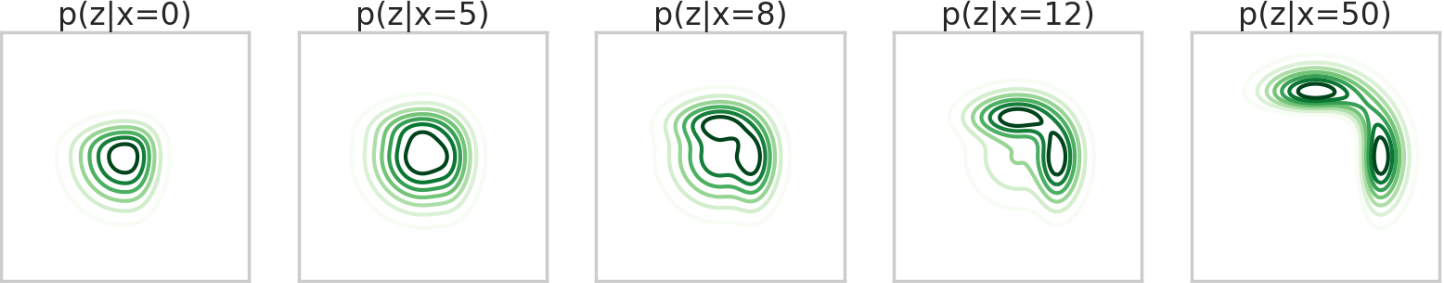
\includegraphics[width=\textwidth]{sprinklertrue.png}
\caption{\small This figure depicts the true (unnormalised) posterior plots for the ``Continuous Sprinkler" experiment. As $x$ increases, the posteriors become increasingly bi-modal and unusually shaped.}
\label{fig:6.1}
\end{figure}
\section{Program Structure}
Recall from \autoref{sec:3.8.1} that our generator $\mathcal{G}_\phi(x,\varepsilon)$ is a neural network that takes in noise $\varepsilon\sim \pi(\varepsilon)$ along with a data sample $x\sim q^*(x)$, outputting a sample from the variational posterior density $\bm{z}\sim q_\phi(\bm{z}|x)$. In this experiment, the generator has 3 noise inputs $\bm{\varepsilon}=(\varepsilon_1,\varepsilon_2,\varepsilon_3)^\top \sim \mathcal{N}(0,I_{3\times 3})$ along with 1 data input $x$, and 2 posterior outputs $z_1, z_2$. The structure of this network is as depicted in \autoref{fig:6.2}. In the figure, the number inside the node indicates how many nodes the layer has, and the text above the node describes the activation function. Recall that the input layer does not have an activation function, and that Rectified Linear Units (ReLU) are used for most of the hidden layers due to their many advantages. In the Concat. layer, the two input vectors are concatenated and there is no activation function.
\begin{figure}[h!]
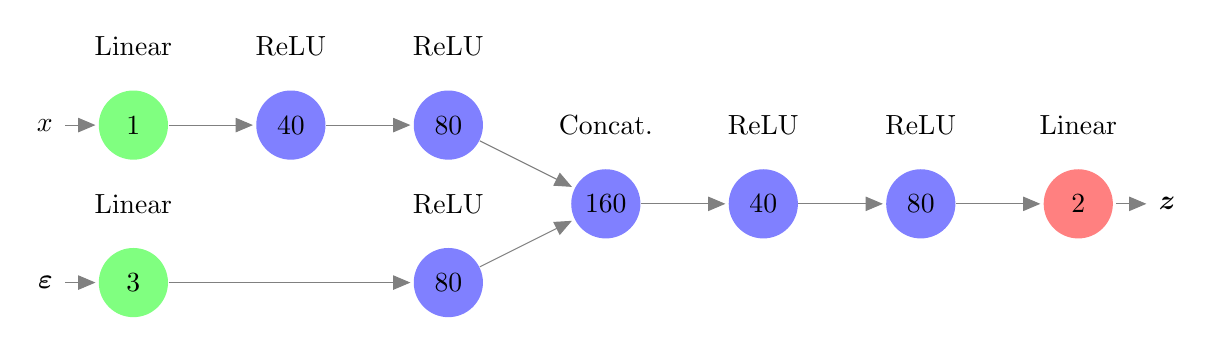
\begin{tikzpicture}[shorten >=1pt,->,draw=black!50, node distance=2.5cm]
    \tikzstyle{every pin edge}=[<-,shorten <=1pt]
    \tikzstyle{neuron}=[circle,fill=black!25,minimum size=25pt,inner sep=0pt]
    \tikzstyle{input neuron}=[neuron, fill=green!50];
    \tikzstyle{output neuron}=[neuron, fill=red!50];
    \tikzstyle{hidden neuron}=[neuron, fill=blue!50];
    \tikzstyle{annot} = [text width=4em, text centered]
    
	%\node[input neuron, pin=left:Bias] (I-0) at (0,0) {$x_0$};
    % Draw the input layer nodes
    %\foreach \name / \y in {1,...,3}
    % This is the same as writing \foreach \name / \y in {1/1,2/2,3/3,4/4}
    \node[input neuron, pin=left:$x$] (I-1) at (0,-1) {$1$};
	\node[input neuron, pin=left:$\bm{\varepsilon}$] (I-2) at (0,-3) {$3$};

    \path[yshift=0cm] node[hidden neuron] (H-11) at (2.0cm,-1) {$40$};
	\path[yshift=0cm] node[hidden neuron] (H-12) at (4.0cm,-1) {$80$};
    \path[yshift=0cm] node[hidden neuron] (H-2) at (4.0cm,-3) {$80$};
    \path[yshift=0cm] node[hidden neuron] (H-3) at (6.0cm,-2) {$160$};
    \path[yshift=0cm] node[hidden neuron] (H-31) at (8.0cm,-2) {$40$};
    \path[yshift=0cm] node[hidden neuron] (H-32) at (10.0cm,-2) {$80$};
	\path[yshift=0cm] node[output neuron,pin={[pin edge={->}]right:$\bm{z}$}] (O) at (12.0cm, -2) {$2$};
    \path (I-1) edge (H-11);
    \path (H-11) edge (H-12);
	\path (I-2) edge (H-2);
	\path (H-12) edge (H-3);
	\path (H-2) edge (H-3);
	\path (H-3) edge (H-31);
	\path (H-31) edge (H-32);
	\path (H-32) edge (O);
    % Annotate the layers
    \node[annot,above of=I-1, node distance=1cm] {Linear};
    \node[annot,above of=I-2, node distance=1cm] {Linear};
    \node[annot,above of=H-11, node distance=1cm] {ReLU};
    \node[annot,above of=H-12, node distance=1cm] {ReLU};
    \node[annot,above of=H-2, node distance=1cm] {ReLU};
    \node[annot,above of=H-3, node distance=1cm] {Concat.};
    \node[annot,above of=H-31, node distance=1cm] {ReLU};
    \node[annot,above of=H-32, node distance=1cm] {ReLU};
    \node[annot,above of=O, node distance=1cm] {Linear};
\end{tikzpicture}
\caption{\small This figure illustrates the structure of the generator network $\mathcal{G}(x,\bm{\varepsilon})$ used in the ``Continuous Sprinkler" experiment. We do not use an activation function for the output layer as $\bm{z}\in \R^2$.}
\label{fig:6.2}
\end{figure}

The structure of the estimator (discriminator $D_\alpha(\bm{z},x)$, direct ratio estimator $r_\alpha(\bm{z},x)$ or direct log ratio estimator $T_\alpha(\bm{z},x)$) is similar to that of the generator, with an additional hidden layer associated with the $\bm{z}$ input and a different output activation function corresponding to the estimator's identity. When the estimator takes the parametrization of a discriminator $D_\alpha(\bm{z},x)$, a sigmoid output layer is used \citep{gan}. An exponential activation function $g(x)={\rm e}^x$ is used for the output layer when the estimator output is the direct density ratio $r_\alpha(\bm{z},x)$, and a linear output is used for the direct log density ratio estimator $T_\alpha(\bm{z},x)$ \citep{nowozin}. The estimator structure is shown in \autoref{fig:6.3}.
\begin{figure}[h!]

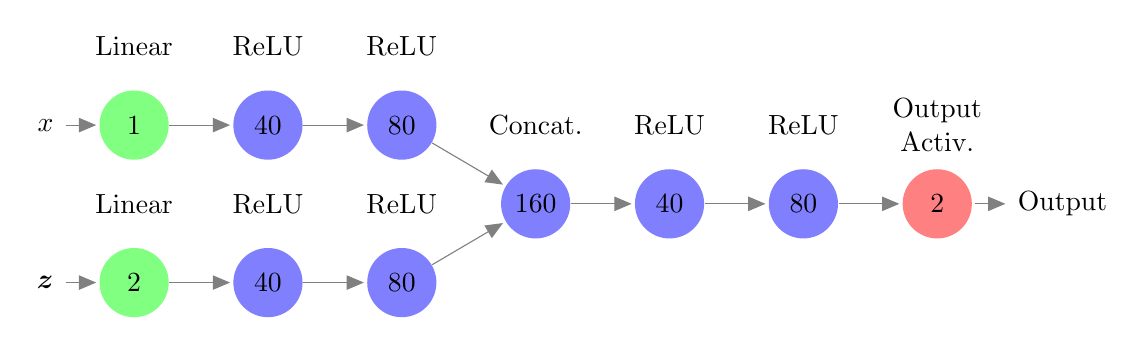
\begin{tikzpicture}[shorten >=1pt,->,draw=black!50, node distance=2.5cm]
    \tikzstyle{every pin edge}=[<-,shorten <=1pt]
    \tikzstyle{neuron}=[circle,fill=black!25,minimum size=25pt,inner sep=0pt]
    \tikzstyle{input neuron}=[neuron, fill=green!50];
    \tikzstyle{output neuron}=[neuron, fill=red!50];
    \tikzstyle{hidden neuron}=[neuron, fill=blue!50];
    \tikzstyle{annot} = [text width=4em, text centered]
    
	%\node[input neuron, pin=left:Bias] (I-0) at (0,0) {$x_0$};
    % Draw the input layer nodes
    %\foreach \name / \y in {1,...,3}
    % This is the same as writing \foreach \name / \y in {1/1,2/2,3/3,4/4}
    \node[input neuron, pin=left:$x$] (I-1) at (0,-1) {$1$};
	\node[input neuron, pin=left:$\bm{z}$] (I-2) at (0,-3) {$2$};

    \path[yshift=0cm] node[hidden neuron] (H-11) at (1.7cm,-1) {$40$};
	\path[yshift=0cm] node[hidden neuron] (H-12) at (3.4cm,-1) {$80$};
	\path[yshift=0cm] node[hidden neuron] (H-21) at (1.7cm,-3) {$40$};
    \path[yshift=0cm] node[hidden neuron] (H-22) at (3.4cm,-3) {$80$};
    \path[yshift=0cm] node[hidden neuron] (H-3) at (5.1cm,-2) {$160$};
    \path[yshift=0cm] node[hidden neuron] (H-31) at (6.8cm,-2) {$40$};
    \path[yshift=0cm] node[hidden neuron] (H-32) at (8.5cm,-2) {$80$};
	\path[yshift=0cm] node[output neuron,pin={[pin edge={->}]right:Output}] (O) at (10.2cm, -2) {$2$};
    \path (I-1) edge (H-11);
    \path (H-11) edge (H-12);
	\path (I-2) edge (H-21);
	\path (H-21) edge (H-22);
	\path (H-12) edge (H-3);
	\path (H-22) edge (H-3);
	\path (H-3) edge (H-31);
	\path (H-31) edge (H-32);
	\path (H-32) edge (O);
    % Annotate the layers
    \node[annot,above of=I-1, node distance=1cm] {Linear};
    \node[annot,above of=I-2, node distance=1cm] {Linear};
    \node[annot,above of=H-11, node distance=1cm] {ReLU};
    \node[annot,above of=H-12, node distance=1cm] {ReLU};
    \node[annot,above of=H-21, node distance=1cm] {ReLU};
    \node[annot,above of=H-22, node distance=1cm] {ReLU};
    \node[annot,above of=H-3, node distance=1cm] {Concat.};
    \node[annot,above of=H-31, node distance=1cm] {ReLU};
    \node[annot,above of=H-32, node distance=1cm] {ReLU};
    \node[annot,above of=O, node distance=1cm] {Output Activ.};
\end{tikzpicture}
\caption{\small This figure depicts the structure of the estimator network for the ``Continuous Sprinkler Experiment". The notation is the same as in \autoref{fig:6.2}. Note that the only differences between the estimators are the activation function of their output layers and the loss functions used to train them.}
\label{fig:6.3}
\end{figure}

The network weights are initialized with Xavier initialization (as explained in \autoref{sec:2.5}), and trained using the Adam optimizer (described in \autoref{sec:2.6}) with learning rate $0.0001$ for the prior-contrastive setting and $0.00001$ for the joint-contrastive algorithms. These values were determined via trial and error to yield consistent results. Recall from the nature of our dataset density $q^*(x)$ that we only train the network on data values $x=0,5,8,12,50$. In each training iteration, 200 samples are taken for each $x$-value, corresponding to a batch size of 1000. This large batch size makes training more consistent, as the latent variables $\bm{z}$ are probabilistic in nature. Due to the similar network structure in each algorithm, they have near-identical runtime, as the majority of the training time is spent in back-propagation \citep{DeepLearning}.

To prevent taking $\log 0$ in the loss functions, we add a constant $c=10^{-18}$ to the log function's input. Preliminary tests show that this sufficiently small constant does not have an apparent effect on the program's performance. The estimator is pre-trained for 5000 iterations to ensure that optimization of the variational network begins with an optimal estimator. The variance of the results is also reduced as the initial parametrization of the estimator is similar for each fixed generator initialization. Afterwards, the variational posterior is optimized for 10000 iterations for the prior-contrastive experiment, and 40000 iterations in the joint-contrastive formulation. Again, these values were chosen through trial and error to result in sufficient posterior convergence. Between each of these iterations, the algorithm takes 100 training steps of the estimator. Pseudocode for the prior-contrastive and joint-contrastive algorithms, based off their derivations in Chapters \ref{ch4} and \ref{ch5}, are shown in Algorithms \ref{alg:7} and \ref{alg:8} in \autoref{app:B.3}.

We evaluate the algorithms by comparing the level of posterior convergence. To measure this, we use the average `true' KL divergence between the true and variational posteriors at the end of the program's runtime: \[\E_{q^*(x)}\left[KL(q_\phi(\bm{z}|x)\|p(\bm{z}|x))\right].\] To do so, we estimate the probability density function of the variational posterior for each of the 5 data points using a Gaussian kernel density estimator $\hat{q}(\bm{z}|x)$. We then calculate its expected KL divergence with the unnormalised true posterior derived in Equation (6.2.1). The normalisation constant $p(x)$ is independent of the variational posterior $q_\phi(\bm{z}|x)$ that we compare it with, so its omission does not affect our comparison of the algorithms. An explanation of kernel density estimation can be found in \autoref{app:D}. Due to the stochastic nature of the optimization, it is desirable to have a large number of experiment repetitions for reliable results. However, due to limited computational time, each algorithm was only run 30 times. At the end of each posterior optimization step, both the estimator loss and $NELBO$ estimation were stored. Additionally, the `true' KL divergence was estimated every 100 posterior iterations. Arrays containing these values were averaged over the 30 experiment repetitions, and plotted as shown in Section 6.4.
\section{Results}
Tables \ref{tab:6.1} and \ref{tab:6.2} compare the `true' KL divergence between the 30 iterations for each algorithm variation. \autoref{fig:6.4} compares variational posterior output plots corresponding to different `true' KL divergences. In the prior-contrastive context, there is no major difference in posterior convergence for the algorithms, and the variation in the results is very low. However, \autoref{fig:6.4} suggests that the variational posterior reaches optimality at the `true' KL divergence of around 1.326. This was verified by running a prior-contrastive algorithm for twice as long (20000 posterior iterations) and observing that the metric did not decrease any further. We can therefore deduce that all of the prior-contrastive programs reached optimality, so we cannot draw any conclusions from those results. It is intuitive that explicit knowledge of the likelihood density in the prior-contrastive algorithm leads to faster posterior convergence than in the joint-contrastive experiments. Plots corresponding to the prior-contrastive optimal estimator experiment can be found in \autoref{app:E}.

Figures \ref{fig:6.5}-\ref{fig:6.7} correspond to the average KL divergence, estimator loss and estimated $NELBO$ over the runtime of the program for the joint-contrastive cases. In these figures, there is little relative difference between the estimator parametrizations. Note that the relative trend in the estimator loss plot is reflected in the corresponding $NELBO$ plot.

\begin{figure}[h!]
\begin{subfigure}{\textwidth}
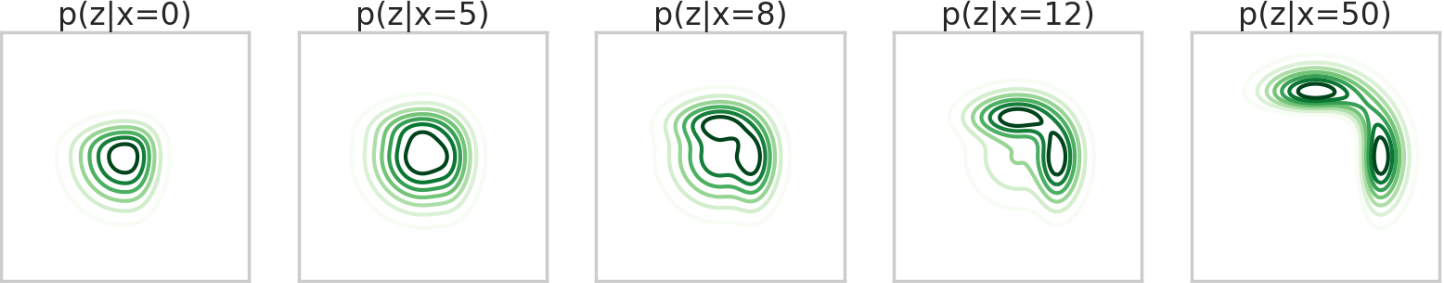
\includegraphics[width=\linewidth]{sprinklertrue.png}
\caption{True Posterior Plot}
\end{subfigure}
\begin{subfigure}{\textwidth}
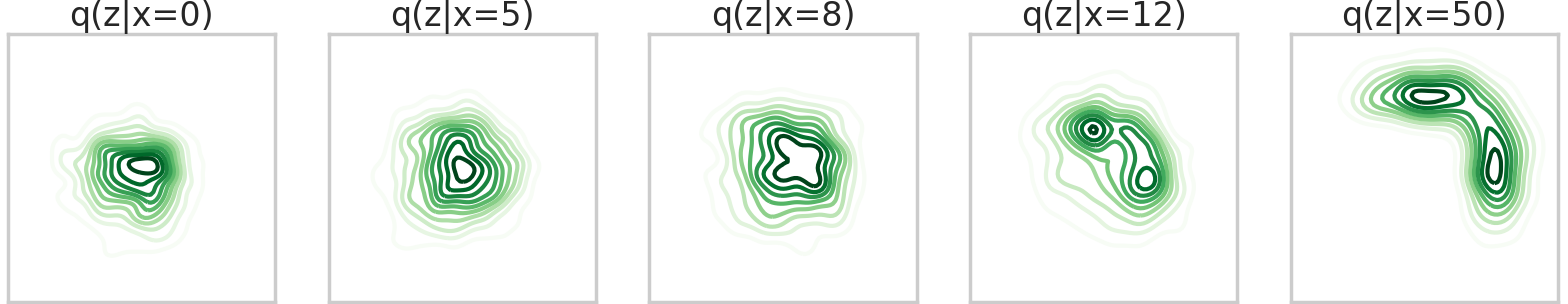
\includegraphics[width=\linewidth]{13288.png}
\caption{Variational Posterior Plot with `True' KL Divergence of 1.3288}
\end{subfigure}
\begin{subfigure}{\textwidth}
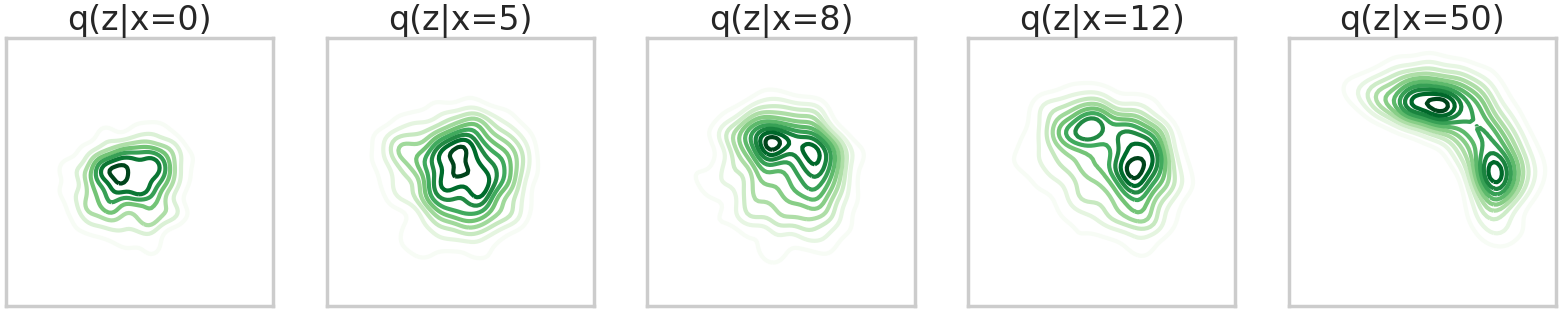
\includegraphics[width=\linewidth]{13623.png}
\caption{Variational Posterior Plot with `True' KL Divergence of 1.3623}
\end{subfigure}
\begin{subfigure}{\textwidth}
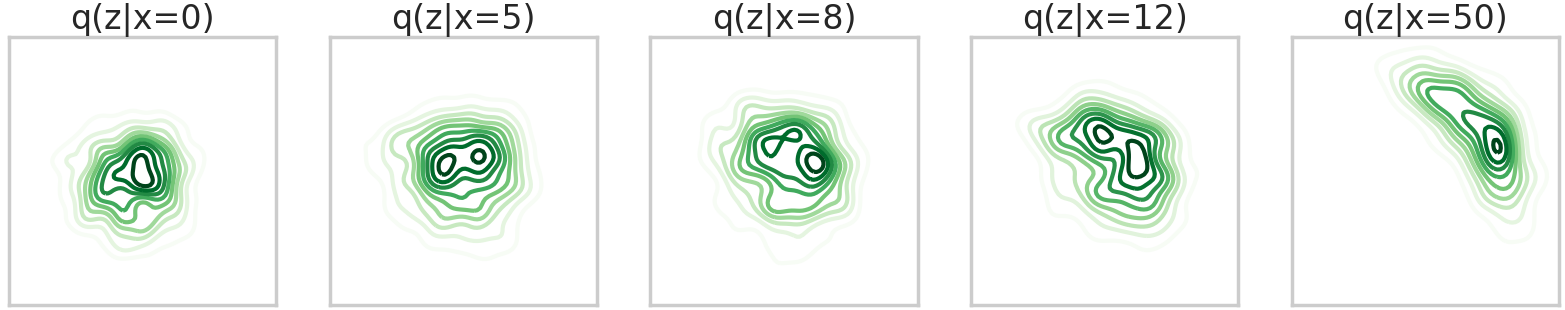
\includegraphics[width=\linewidth]{13963.png}
\caption{Variational Posterior Plot with `True' KL Divergence of 1.3963}
\end{subfigure}
\caption{\small Above we compare the true (unnormalised) posterior as plotted in \autoref{fig:6.1} against variational posterior outputs corresponding to varying KL divergences. Sub-figures (b)-(d) were created by fitting a Gaussian kernel density estimation over 1000 posterior samples. Note that the variational posterior is relatively optimal at a `true' KL divergence of 1.3288, and that the output appears less flexible as the divergence increases. In sub-figure (d), the variational posterior fails to capture the bimodality of the true posterior.}
\label{fig:6.4}
\end{figure}
\newpage

\begin{table}[t!]
\centering
\begin{tabular}{|l|c|c|c|}
\hline
\multicolumn{4}{|c|}{Prior-Contrastive Results}\\
\hline
\multicolumn{2}{|c|}{Algorithm} & Mean KL Divergence & Standard Deviation\\
\hline
\multirow{3}{*}{Reverse KL} & $D_\alpha(\bm{z},x)$ & 1.3271 & 0.0041\\
\cline{2-4}
& $r_\alpha(\bm{z},x)$ & 1.3265 & 0.0045\\
\cline{2-4}
& $T_\alpha(\bm{z},x)$ & 1.3262 & 0.0041\\
\hline
\multirow{3}{*}{GAN} & $D_\alpha(\bm{z},x)$ & 1.3267 & 0.0041\\
\cline{2-4}
& $r_\alpha(\bm{z},x)$ & 1.3263 & 0.0035\\
\cline{2-4}
& $T_\alpha(\bm{z},x)$ & 1.3258 & 0.0039\\
\hline
\end{tabular}
\caption{\small This table presents the results from the prior-contrastive experiment. Since the programs reached optimality in this case, it is uncertain from those results whether the choice of $f$-divergence or estimator parametrization impacts posterior convergence.}
\label{tab:6.1}
\end{table}

\begin{table}[h!]
\centering
\begin{tabular}{|l|c|c|c|}
\hline
\multicolumn{4}{|c|}{Joint-Contrastive Results}\\
\hline
\multicolumn{2}{|c|}{Algorithm} & Mean KL Divergence & Standard Deviation\\
\hline
\multirow{3}{*}{Reverse KL} & $D_\alpha(\bm{z},x)$ & \textbf{1.3416} & \textbf{0.0068}\\
\cline{2-4}
& $r_\alpha(\bm{z},x)$ & \textbf{1.3397} & \textbf{0.0066}\\
\cline{2-4}
& $T_\alpha(\bm{z},x)$ & \textbf{1.3446} & 0.0108\\
\hline
\multirow{3}{*}{GAN} & $D_\alpha(\bm{z},x)$ & 1.3648 & 0.0242\\
\cline{2-4}
& $r_\alpha(\bm{z},x)$ & 1.3657 & 0.0302\\
\cline{2-4}
& $T_\alpha(\bm{z},x)$ & 1.3670 & 0.0387\\
\hline
\end{tabular}
\caption{\small From these joint-contrastive results, it is evident that for each $f$-divergence, similar posterior convergence is associated with the different estimator parametrizations. As ``$f$-GAN: Training Generative Neural Samplers using Variational Divergence Minimization" by \citet{nowozin} suggests, the GAN divergence demonstrates slower and more inconsistent results than the reverse KL divergence.}
\label{tab:6.2}
\end{table}
\begin{figure}[h!]
\begin{subfigure}{0.49\textwidth}
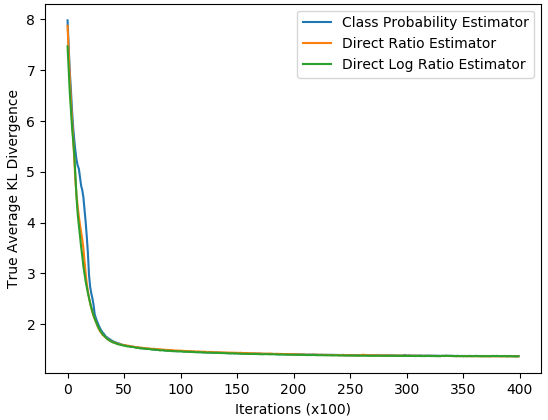
\includegraphics[width=\linewidth]{truklmins/JCADVvsJCADVexpvsJCADVgudlog.png}
\caption{GAN Divergence}
\end{subfigure}
\begin{subfigure}{0.49\textwidth}
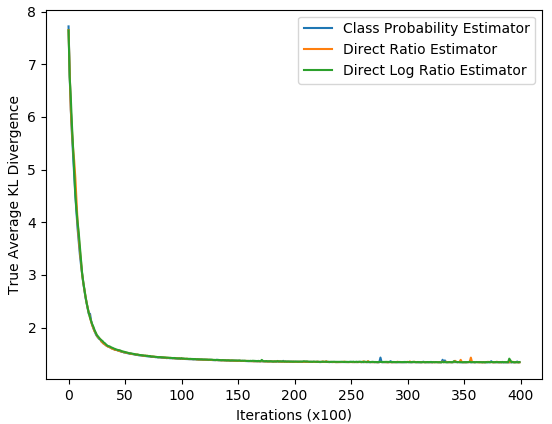
\includegraphics[width=\linewidth]{truklmins/JCKLDvsJCKLexpvsJCKLgudlog.png}
\caption{Reverse KL Divergence}
\end{subfigure}
\caption{\small These plots of the true KL divergence in the joint-contrastive context show near identical convergence for all estimators.}
\label{fig:6.5}
\end{figure}
\newpage
\begin{figure}
\begin{subfigure}{0.49\textwidth}
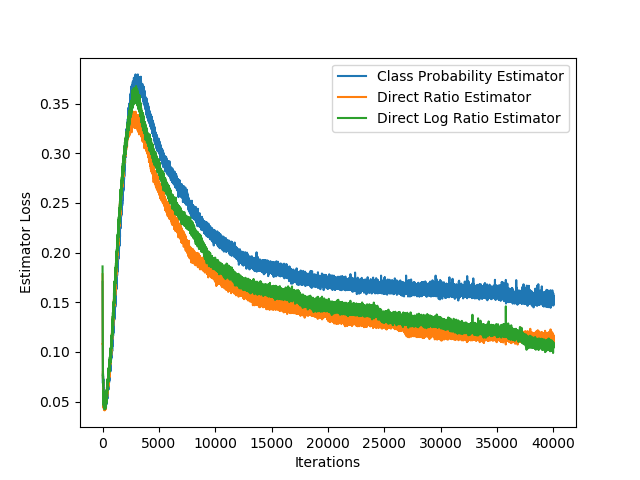
\includegraphics[width=\linewidth]{estimator_losses/JCADVvsJCADVexpvsJCADVgudlog.png}
\caption{GAN Divergence}
\end{subfigure}
\begin{subfigure}{0.49\textwidth}
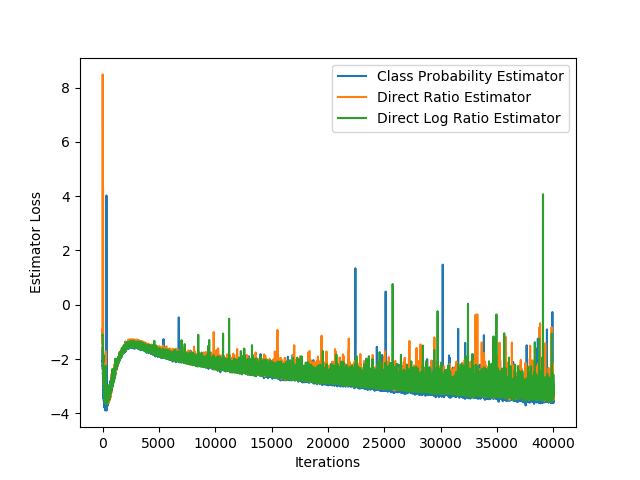
\includegraphics[width=\linewidth]{estimator_losses/JCKLDvsJCKLexpvsJCKLgudlog.png}
\caption{Reverse KL Divergence}
\end{subfigure}
\caption{\small In sub-figure (a), the estimators have similar levels of stability, but the class probability estimator loss appears to be higher than the other two estimator parametrizations. This does not appear to affect posterior convergence. All three estimators formulated by the reverse KL divergence have similar, increasingly unstable losses.}
\label{fig:6.6}
\end{figure}

\begin{figure}
\begin{subfigure}{0.49\textwidth}
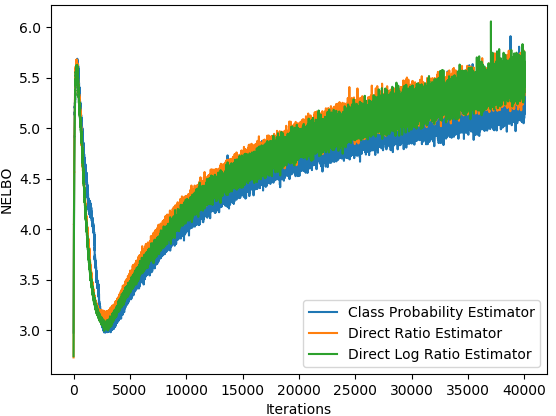
\includegraphics[width=\linewidth]{nelbos/JCADVvsJCADVexpvsJCADVgudlog.png}
\caption{GAN Divergence}
\end{subfigure}
\begin{subfigure}{0.49\textwidth}
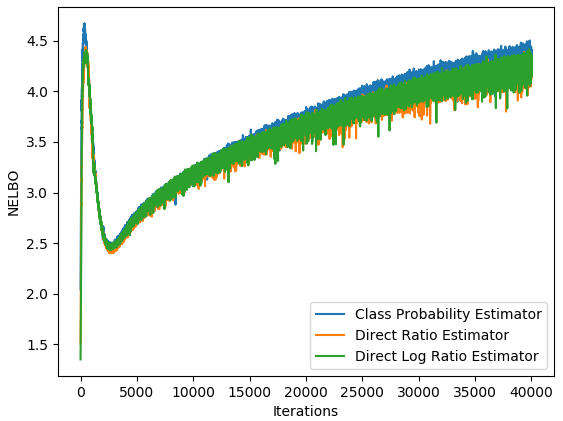
\includegraphics[width=\linewidth]{nelbos/JCKLDvsJCKLexpvsJCKLgudlog.png}
\caption{Reverse KL Divergence}
\end{subfigure}
\caption{\small These joint-contrastive $NELBO$ plots generally mirror the estimator loss trends depicted in \autoref{fig:6.6}. Lower and more stable $NELBO$ estimations are associated with the reverse KL divergence, correlating with its superior posterior convergence. It is unclear why the $NELBO$ increases over the iterations when its minimization theoretically leads to posterior convergence.}
\label{fig:6.7}
\end{figure}
\chapter{Comparing Undertrained Estimators}\label{ch7}
Since all three estimator parametrizations have similar accuracies at optimality, it does not matter which one is chosen in that context. However, insufficient estimator training iterations can lead to an inaccurate $NELBO$ estimation, reducing the speed at which the variational posterior converges. In this chapter, we theoretically compare the estimator convergence rates between the three parametrizations by analysing the bounds of the estimator outputs, the second functional derivatives of their loss functions and the displacement in the optimal estimator output with each posterior optimization step. We then compare the performance of undertrained estimators with different parametrizations and $f$-divergence lower bounds.
\section{Theory}\label{sec:7.1}
\subsection{Estimator Bounds}
Consider the bounds on the estimator outputs. The class probability estimator $D_\alpha(u)\simeq q(u)/(q(u)+p(u))$ is bound in $(0,1)$, so from any arbitrary starting point in the same space, very few optimization steps are required to reach the global minimum. On the other hand, the direct ratio estimator $r_\alpha(u)\simeq q(u)/p(u)$ can only output values in $(0,\infty)$, and the direct log ratio estimator $T_\alpha(u) \simeq \log (q(u)/p(u))$ can output any value in $\R$, so optimization can take many iterations if the difference between the estimator's initial and optimal values is too large. This can be problematic if there are insufficient iterations of optimizing the estimator, particularly in the initialization stage: the estimator may not properly converge and the posterior will be trained with an inaccurate density ratio estimation. Essentially, the gradient descent convergence can be improved by using an appropriate transformation \citep{lecun}.

By converting the loss functions to integral form, we are able to visualise the bounds on the loss function output by fixing $q(u)$ and $p(u)$ as arbitrary values in $(0,1)$, and plotting the functional inside the integral. \autoref{fig:7.1} depicts plots of estimator outputs against the loss functional where $q(u)=p(u)=0.5$.
\begin{example}
In this example we formulate the loss functional plotted in \autoref{fig:7.1} (a): the class probability estimator $D_\alpha(u)$ derived from the GAN divergence. The relevant estimator loss function is:
\begin{align*}
-\E_{q(u)}[\log D_\alpha(u)]-\E_{p(u)}[\log (1-D_\alpha(u))]&=\int_U -q(u)\log D_\alpha(u)\\
&\quad \quad -p(u)\log(1-D_\alpha(u)) \,{\rm d}u\\
&=\int_U -\frac{\log D_\alpha(u)+\log(1-D_\alpha(u))}{2}\,{\rm d}u.
\end{align*}
In the derivation above we have set $q(u)=p(u)=0.5$. Note we plot the functional inside the integral:
\[f(u)=-\frac{\log D_\alpha(u)+\log(1-D_\alpha(u))}{2}.\]
\end{example}
\begin{figure}[h!]
\begin{subfigure}{0.49\textwidth}
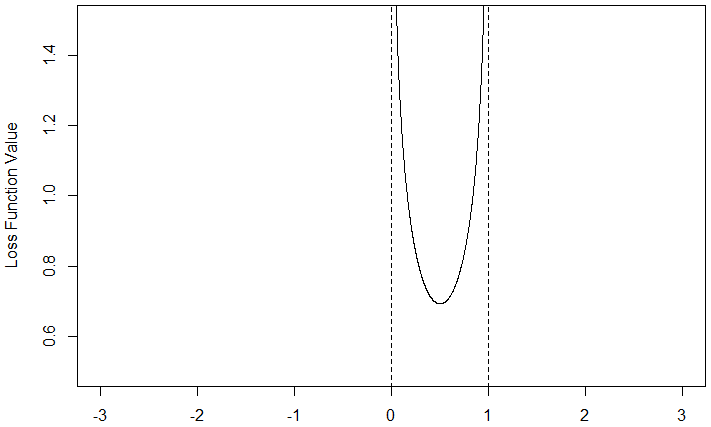
\includegraphics[width=\linewidth]{ADVD.png}
\caption{GAN Divergence - $D_\alpha(u)$}
\end{subfigure}
\begin{subfigure}{0.49\textwidth}
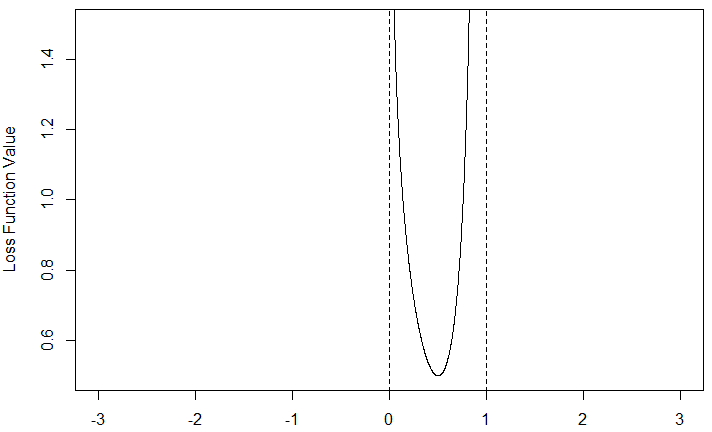
\includegraphics[width=\linewidth]{KLD.png}
\caption{Reverse KL Divergence - $D_\alpha(u)$}
\end{subfigure}
\begin{subfigure}{0.49\textwidth}
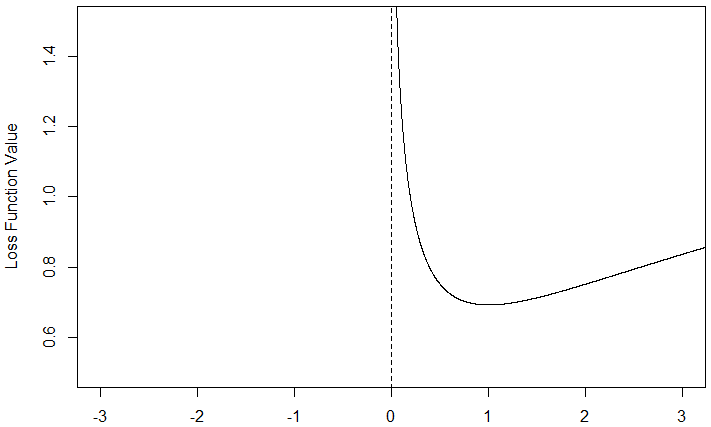
\includegraphics[width=\linewidth]{ADVR.png}
\caption{GAN Divergence - $r_\alpha(u)$}
\end{subfigure}
\begin{subfigure}{0.49\textwidth}
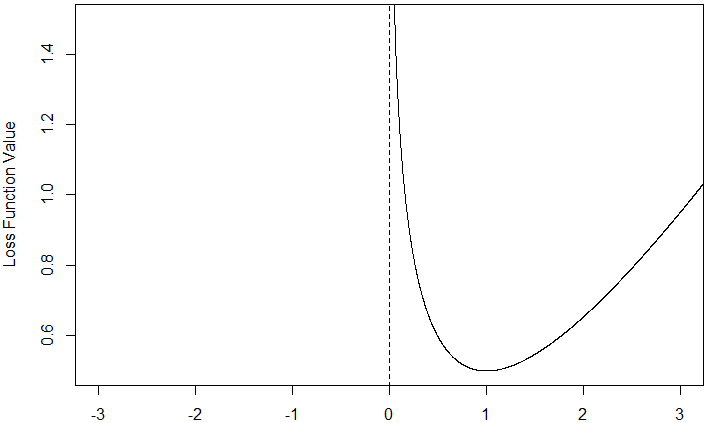
\includegraphics[width=\linewidth]{KLR.png}
\caption{Reverse KL Divergence - $r_\alpha(u)$}
\end{subfigure}
\begin{subfigure}{0.49\textwidth}
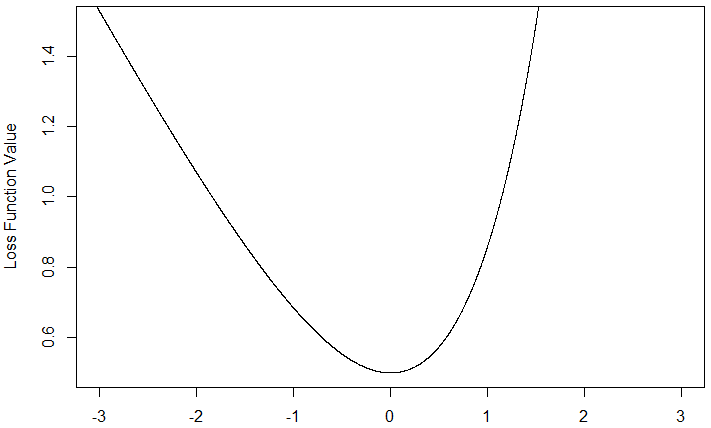
\includegraphics[width=\linewidth]{ADVT.png}
\caption{GAN Divergence - $T_\alpha(u)$}
\end{subfigure}
\begin{subfigure}{0.49\textwidth}
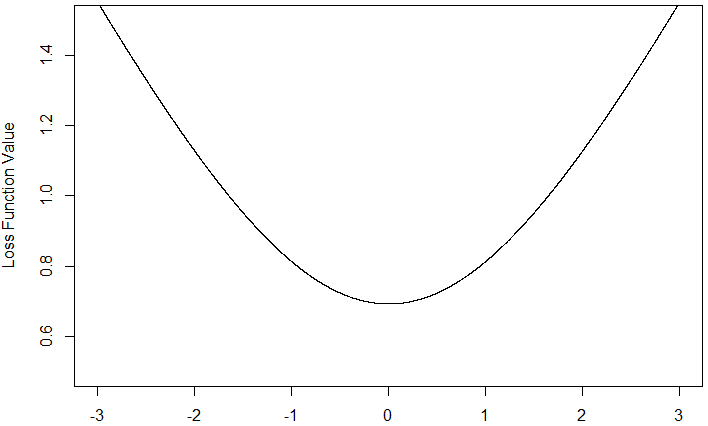
\includegraphics[width=\linewidth]{KLT.png}
\caption{Reverse KL Divergence - $T_\alpha(u)$}
\end{subfigure}
\caption{\small Above we have plotted the estimator output against its loss functional. The same $x$ and $y$-axis scales are used for all plots. Due to the bounds, it is evident that the loss functionals using the class probability estimator $D_\alpha(u)$ are associated with the highest gradient values and therefore the fastest convergence. It is difficult to compare the direct ratio estimator $r_\alpha(u)$ and the direct log ratio estimator $T_\alpha(u)$, as the former estimator appears to have higher gradients when $q(u)<p(u)$, but slower convergence when $q(u)>p(u)$. Since the relative gradients of the graph can vary with the choice of $p(u)$ and $q(u)$, we cannot compare the $f$-divergences.}
\label{fig:7.1}
\end{figure}
\subsection{First and Second Derivatives of Estimator Loss Functions}
It is known that the convergence rate of a gradient descent method is proportional to the size of its second derivative \citep{lecun}, hence we can use it to compare our algorithms. Below we formulate the second functional derivatives of the estimator losses with respect to the estimator function. It can be shown that the conditions to take the first and second functional derivative using the Euler-Lagrange equation are met. Due to the exponential term in the direct log ratio estimator loss functions, it is difficult to compare their second derivatives, hence we omit them in this section. Their derivations can be found in \autoref{app:F}. 
\subsubsection*{\textbf{Reverse KL Divergence Bound}:}
Class Probability Estimator:
\begin{align*}
L_{RKL}(u)&\coloneqq-\E_{q(u)}\left[\log \frac{D_\alpha(u)}{1-D_\alpha(u)}\right]+\E_{p(u)}\left[\frac{D_\alpha(u)}{1-D_\alpha(u)}\right]\\
&=-\int_U q(u)\left(\log \frac{D_\alpha(u)}{1-D_\alpha(u)}\right)\,{\rm d}u+\int_U p(u)\left(\frac{D_\alpha(u)}{1-D_\alpha(u)}\right)\,{\rm d}u.\\
\frac{\partial L_{RKL}(u)}{\partial D_\alpha(u)}&=-\frac{q(u)}{D_\alpha(u)}-\frac{q(u)}{1-D_\alpha(u)}+\frac{p(u)}{1-D_\alpha(u)}+\frac{p(u)D_\alpha(u)}{(1-D_\alpha(u))^2}\\
&=-\frac{q(u)}{D_\alpha(u)}-\frac{q(u)}{1-D_\alpha(u)}+\frac{p(u)}{(1-D_\alpha(u))^2}.\\
\frac{\partial^2L_{RKL}(u)}{\partial D_\alpha^2(u)}&=\frac{q(u)}{D_\alpha^2(u)}-\frac{q(u)}{(1-D_\alpha(u))^2}+\frac{2p(u)}{(1-D_\alpha(u))^3}.
\end{align*}
Direct Ratio Estimator:
\begin{align}
L_{RKL}(u)&\coloneqq-\E_{q(u)}[\log r_\alpha(u)]+\E_{p(u)}[r_\alpha(u)]\nonumber\\
&=-\int_U q(u)\log r_\alpha(u) \,{\rm d}u+\int_U p(u)r_\alpha(u)\,{\rm d}u.\nonumber\\
\frac{\partial L_{RKL}(u)}{\partial r_\alpha(u)}&=-\frac{q(u)}{r_\alpha(u)}+p(u).\nonumber\\
\frac{\partial^2L_{RKL}(u)}{\partial r_\alpha^2(u)}&=\frac{q(u)}{r_\alpha^2(u)}.
\end{align}
\subsubsection*{\textbf{GAN Divergence Bound}:}
Class Probability Estimator:
\begin{align}
L_{GAN}(u)&\coloneqq-\E_{q(u)}[\log D_\alpha(u)]-\E_{p(u)}[\log (1-D_\alpha(u))]\nonumber\\
&=-\int_U q(u)\log D_\alpha(u) \,{\rm d}u -\int_U p(u)\log(1-D_\alpha(u))\,{\rm d}u.\nonumber\\
\frac{\partial L_{GAN}(u)}{\partial D_\alpha(u)}&=-\frac{q(u)}{D_\alpha(u)}+\frac{p(u)}{1-D_\alpha(u)}.\nonumber\\
\frac{\partial^2L_{GAN}(u)}{\partial D_\alpha^2(u)}&=\frac{q(u)}{D_\alpha^2(u)}+\frac{p(u)}{(1-D_\alpha(u))^2}.
\end{align}
Direct Ratio Estimator:
\begin{align}
L_{GAN}(u)&\coloneqq-\E_{q(u)}\left[\log \frac{r_\alpha(u)}{r_\alpha(u)+1}\right]+\E_{p(u)}\left[\log(r_\alpha(u)+1)\right]\nonumber\\
&=-\int_U q(u)\left[\log \frac{r_\alpha(u)}{r_\alpha(u)+1}\right]\,{\rm d}u+\int_U p(u)\left[\log(r_\alpha(u)+1)\right]\,{\rm d}u.\nonumber\\
\frac{\partial L_{GAN}(u)}{\partial r_\alpha(u)}&=-\frac{q(u)}{r_\alpha(u)}+\frac{q(u)}{r_\alpha(u)+1}+\frac{p(u)}{r_\alpha(u)+1}.\nonumber\\
\frac{\partial^2L_{GAN}(u)}{\partial r_\alpha^2(u)}&=\frac{q(u)}{r_\alpha^2(u)}-\frac{q(u)}{(r_\alpha(u)+1)^2}-\frac{p(u)}{(r_\alpha(u)+1)^2}.
\end{align}

By comparing Equations (7.1.2) and (7.1.3), we find that within the GAN divergence, the second derivative of the class probability estimator is strictly superior to that of the direct ratio estimator. Also, a comparison of Equations (7.1.1) and (7.1.3) shows that the direct ratio estimator has a strictly greater second derivative when its loss function is bounded by the reverse KL divergence than with the GAN divergence.
As previously stated, the effectiveness of different $f$-divergence upper bounds has been tested in \citet{nowozin}. They found that the ideal $f$-divergence used for the estimator's loss function is the same $f$-divergence that is being minimized in the variational posterior training: in our case, it is the reverse KL divergence.
\subsection{Displacement of Estimator Optimal Values}
We can also consider the effect of the posterior density displacement from each training step: every time $q(u)$ changes, the optimal parametrization of the estimator also changes. Consequently, the estimator must take optimization steps to reach this new parametrization, but again, if the displacement is too significant, then the estimator may not converge in time.
\begin{lemma}
For a fixed displacement of the variational density $q(u)$, the class probability estimator's global minimum displaces less than the direct ratio estimator, that is, $|D^{*^{(n+1)}}_\alpha(u)-D^{*^{(n)}}_\alpha(u)|<|r^{*^{(n+1)}}_\alpha(u)-r^{*^{(n)}}_\alpha(u)|$:
\begin{proof}
Letting $\varepsilon\neq0$ be the change in $q(u)$ with an optimization step, and assuming that $|\varepsilon|<q(u)$, we have
\begin{align*}
|D^{*^{(n+1)}}_\alpha(u)-D^{*^{(n)}}_\alpha(u)|&=\left|\frac{q(u)+\varepsilon}{q(u)+\varepsilon+p(u)}-\frac{q(u)}{q(u)+p(u)}\right|\\
&=\left|\frac{q^2(u)+q(u)p(u)+\varepsilon q(u)+\varepsilon p(u)}{(q(u)+\varepsilon+p(u))(q(u)+p(u))}\right.\\
&\quad \left.-\frac{q^2(u)+\varepsilon q(u)+q(u)p(u)}{(q(u)+\varepsilon+p(u))(q(u)+p(u))}\right|\\
&=\left|\frac{\varepsilon p(u)}{(q(u)+\varepsilon+p(u))(q(u)+p(u))}\right|\\
&=\left|\frac{\varepsilon}{(q(u)+\varepsilon+p(u))\left(\frac{q(u)}{p(u)}+1\right)}\right|,\\
|r^{*^{(n+1)}}_\alpha(u)-r^{*^{(n)}}_\alpha(u)|&=\left|\frac{q(u)+\varepsilon}{p(u)}-\frac{q(u)}{p(u)}\right|\\
&=\left|\frac{\varepsilon}{p(u)}\right|.
\end{align*}
If $\varepsilon>0$, then
\[|D^{*^{(n+1)}}_\alpha(u)-D^{*^{(n)}}_\alpha(u)|<|r^{*^{(n+1)}}_\alpha(u)-r^{*^{(n)}}_\alpha(u)|\text{ as }(q(u)+\varepsilon+p(u))\left(\frac{q(u)}{p(u)}+1\right)>p(u).\]
If $\varepsilon<0$, then recalling that $|\varepsilon| < q(u) < q(u)+p(u)$,
\begin{align*}
(q(u)+\varepsilon+p(u))(\frac{q(u)}{p(u)}+1)&=\frac{q^2(u)}{p(u)}+2q(u)+p(u)+\varepsilon \left(\frac{q(u)}{p(u)}+1\right)\\
&=(q(u)+\varepsilon)\left(\frac{q(u)}{p(u)}+1\right)+q(u)+p(u)\\
&>p(u).
\end{align*}
\[\implies |D^{*^{(n+1)}}_\alpha(u)-D^{*^{(n)}}_\alpha(u)|<|r^{*^{(n+1)}}_\alpha(u)-r^{*^{(n)}}_\alpha(u)|.\]
\end{proof}
\end{lemma}
\begin{remark}
The class probability estimator $D_\alpha(u)$ requires few optimization steps than the direct ratio estimator $r_\alpha(u)$ to adjust for a fixed change in the variational posterior density.
\end{remark}
For the direct log ratio estimator, we have
\begin{align*}
|T^{*^{(n+1)}}_\alpha(u)-T^{*^{(n)}}_\alpha(u)|&=\left|\log \frac{q(u)+\varepsilon}{p(u)}-\log \frac{q(u)}{p(u)}\right|\\
&=\left|\log \frac{q(u)+\varepsilon}{q(u)}\right|.
\end{align*}
It is difficult to make a direct comparison with the other displacement expressions.

\section{Experiment Outline}
In this experiment, we aim to confirm our theory that the estimator parametrizations have differing density ratio estimation accuracies when improperly trained. We also aim to determine the most accurate undertrained estimator by observing the variational posterior convergence.

The same ``Continuous Sprinkler" experimental setup from \autoref{ch6} is used, but with several changes to the training parameters aimed towards reducing the relative amount of estimator training. We significantly reduce the amount of estimator training, lowering the estimator training rate to 0.00004 and the number of training steps before each posterior iteration to 11 for both contrastive settings. We also increase the posterior training rate to 0.0002 and to account for this change, the number of optimization steps of the variational density is reduced to 2000 for the prior-contrastive context and 4000 in the joint-contrastive algorithms. 
\section{Results}
Tables 7.1 and 7.2, and Figures 7.2\textendash 7.7 present the results in a similar manner to Section 6.4. For each contrastive context and $f$-divergence bound, the class probability estimator $D_\alpha(\bm{z},x)$ consistently demonstrates the lowest mean KL divergence, followed by the direct ratio estimator $r_\alpha (\bm{z},x)$ and the direct log ratio estimator $T_\alpha(\bm{z},x)$. The standard deviation of the results also generally increases with this trend: a lower standard deviation implies more consistent results. These results support the theory presented in \autoref{sec:7.1}, but their significance varies depending on the comparison. Additionally, the estimators formulated by the reverse KL divergence have consistently better results, reinforcing the results in Chapter 6.

The prior-contrastive estimators demonstrate relatively similar results. This is likely because a likelihood term $-\E_{q^*(x)\pi(\varepsilon)}[\log p(x|\mathcal{G}_\phi(\varepsilon;x))]$ is additionally used to optimize the posterior weights $\phi$, so convergence is less dependent on an accurate density ratio estimation. In Figures 7.2\textendash 7.4, we cannot distinguish any noticeable trends between the estimator parametrizations. However, there is an initial instability associated with the estimators formulated with the reverse KL divergence, whilst the GAN divergence corresponds to stable estimators. This observation, in spite of the superiority of the reverse KL divergence, implies a trade-off between the stability and accuracy of an estimator when choosing an $f$-divergence to formulate its loss function.
\begin{table}[h]
\centering
\begin{tabular}{|l|c|c|c|}
\hline
\multicolumn{4}{|c|}{Prior-Contrastive Results}\\
\hline
\multicolumn{2}{|c|}{Algorithm} & Mean KL Divergence & Standard Deviation\\
\hline
\multirow{3}{*}{Reverse KL} & $D_\alpha(\bm{z},x)$ & \textbf{1.3572} & \textbf{0.0136}\\
\cline{2-4}
& $r_\alpha(\bm{z},x)$ & 1.3607 & 0.0199\\
\cline{2-4}
& $T_\alpha(\bm{z},x)$ & 1.3641 & 0.0141\\
\hline
\multirow{3}{*}{GAN} & $D_\alpha(\bm{z},x)$ & 1.3788 & 0.0258\\
\cline{2-4}
& $r_\alpha(\bm{z},x)$ & 1.3811 & 0.0365\\
\cline{2-4}
& $T_\alpha(\bm{z},x)$ & 1.3849 & 0.0450\\
\hline
\end{tabular}
\caption{\small In these prior-contrastive results, it is evident that using the reverse KL divergence to derive the lower bound for the estimator loss function leads to higher posterior convergence, supporting our experimental results in \autoref{ch6}.}
\label{tab:7.1}
\end{table}
\begin{figure}[h]
\begin{subfigure}{0.49\textwidth}
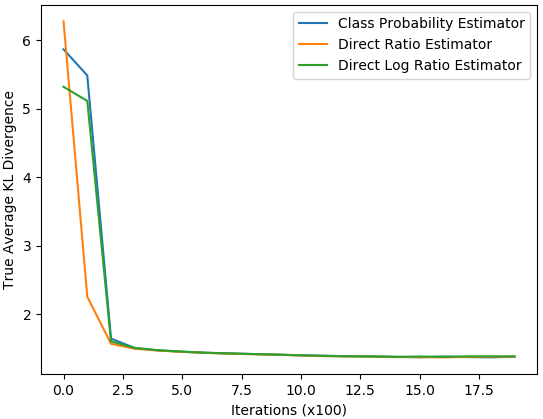
\includegraphics[width=\linewidth]{part2truklmins/PCADVvsPCADVexpvsPCADVgudlog.png}
\caption{GAN Divergence}
\end{subfigure}
\begin{subfigure}{0.49\textwidth}
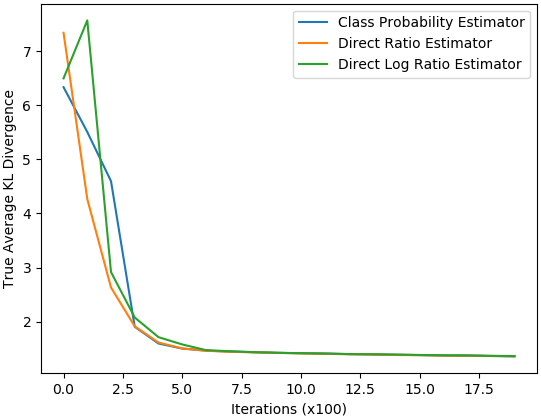
\includegraphics[width=\linewidth]{part2truklmins/PCKLDvsPCKLexpvsPCKLgudlog.png}
\caption{Reverse KL Divergence}
\end{subfigure}
\caption{\small This figure illustrates the reduction in the true average KL divergence over the prior contrastive experiments' runtime. Although the direct ratio estimator plots initially experience a faster reduction, all three estimator plots meet at approximately the same KL divergence. It can be seen that the GAN divergence is associated with a faster initial drop than the reverse KL divergence, yet experiences lower overall posterior convergence.}
\end{figure}
\newpage
\begin{figure}[h]
\begin{subfigure}{0.49\textwidth}
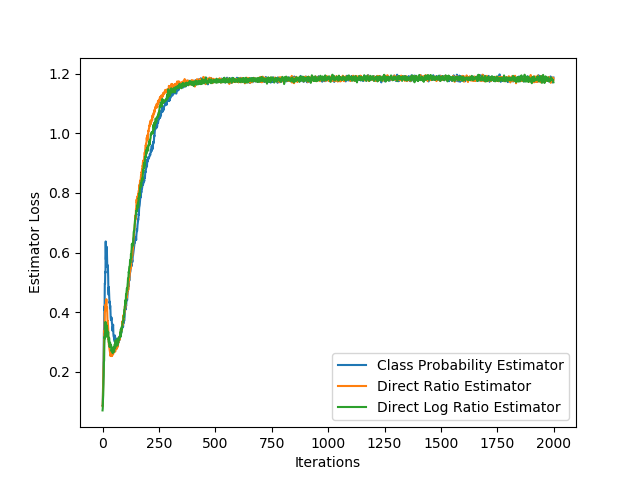
\includegraphics[width=\linewidth]{part2estimatorlosses/PCADVvsPCADVexpvsPCADVgudlog.png}
\caption{GAN Divergence}
\end{subfigure}
\begin{subfigure}{0.49\textwidth}
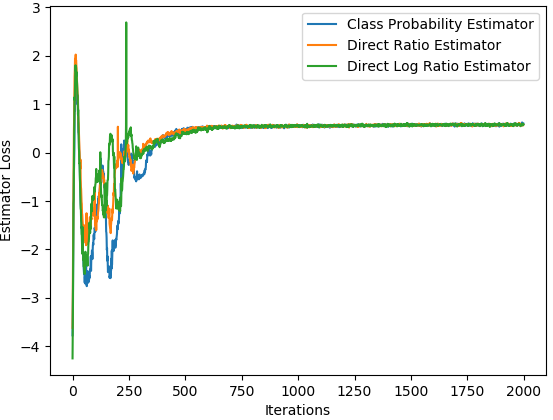
\includegraphics[width=\linewidth]{part2estimatorlosses/PCKLDvsPCKLexpvsPCKLgudlog.png}
\caption{Reverse KL Divergence}
\end{subfigure}
\caption{\small In these prior-contrastive estimator loss plots, it is evident that the estimators bound by the reverse KL divergence experience initial fluctuations which eventually stabilize, whilst the GAN divergence is associated with higher stability. This is consistent with the observations made in Figure 7.2, and implies a trade-off between estimator stability and accuracy in the choice of $f$-divergence.}
\end{figure}
\begin{figure}[h]
\begin{subfigure}{0.49\textwidth}
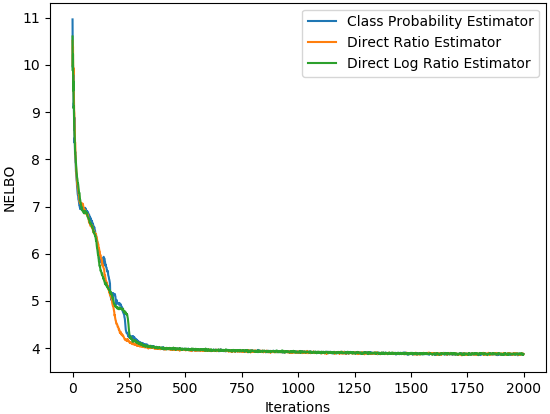
\includegraphics[width=\linewidth]{part2nelbos/PCADVvsPCADVexpvsPCADVgudlog.png}
\caption{GAN Divergence}
\end{subfigure}
\begin{subfigure}{0.49\textwidth}
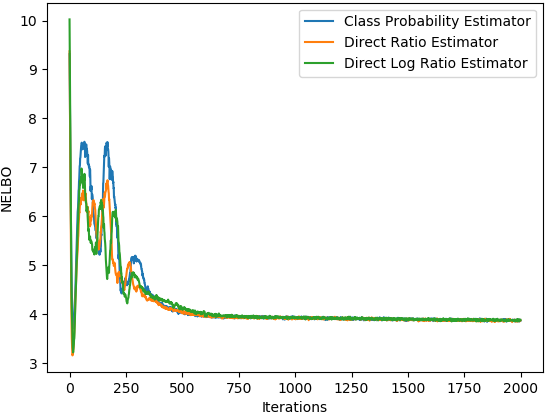
\includegraphics[width=\linewidth]{part2nelbos/PCKLDvsPCKLexpvsPCKLgudlog.png}
\caption{Reverse KL Divergence}
\end{subfigure}
\caption{\small The trends shown in the $NELBO$ plots above are generally consistent with the corresponding estimator loss plots. All of the estimators converge at approximately the same estimated $NELBO$, indicating that the effects of under-training the estimator are mostly experienced in the early program iterations.}
\end{figure}
\newpage
More notable results are found in the joint-contrastive experiments, tabulated in Table \ref{tab:7.2}. This is likely because the entirety of the joint-contrastive $NELBO$ is a density ratio: \[NELBO(q)=\E_{q^*(x)q_\phi(\bm{z}|x)}\left[\frac{q(\bm{z},x)}{p(\bm{z},x)}\right],\] so posterior optimization is more dependent on an accurate density ratio estimation. Similar to the prior-contrastive results, Figures 7.5\textendash 7.7 imply a trade-off between estimator stability and accuracy in the choice of $f$-divergence.
\begin{table}[h]
\centering
\begin{tabular}{|l|c|c|c|}
\hline
\multicolumn{4}{|c|}{Joint-Contrastive Results}\\
\hline
\multicolumn{2}{|c|}{Algorithm} & Mean KL Divergence & Standard Deviation\\
\hline
\multirow{3}{*}{Reverse KL} & $D_\alpha(\bm{z},x)$ & \textbf{1.3786} & \textbf{0.0286}\\
\cline{2-4}
& $r_\alpha(\bm{z},x)$ & 1.3934 & 0.0410\\
\cline{2-4}
& $T_\alpha(\bm{z},x)$ & 1.4133 & 0.0597\\
\hline
\multirow{3}{*}{GAN} & $D_\alpha(\bm{z},x)$ & 1.4017 & \textbf{0.0286}\\
\cline{2-4}
& $r_\alpha(\bm{z},x)$ & 1.4086 & 0.0555\\
\cline{2-4}
& $T_\alpha(\bm{z},x)$ & 1.4214 & 0.0518\\
\hline
\end{tabular}
\caption{\small In these joint-contrastive results, there is a considerable difference between the three estimators when the reverse KL bound is used. However, when the GAN divergence is used to formulate the estimator loss function, only the direct log ratio estimator demonstrates substantially worse posterior convergence than the other two estimators.}
\label{tab:7.2}
\end{table}
\begin{figure}[h]
\begin{subfigure}{0.49\textwidth}
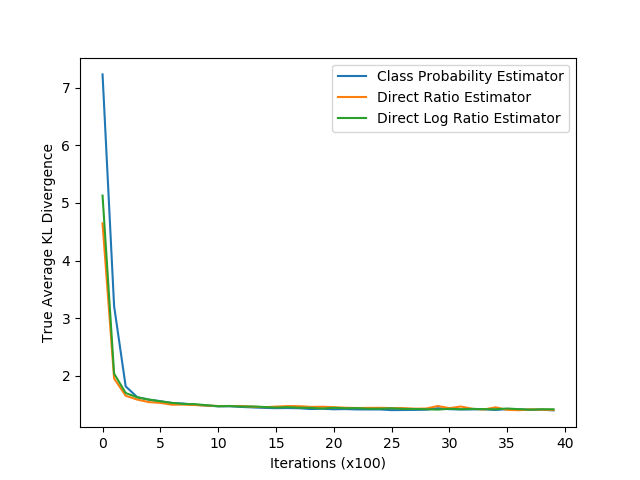
\includegraphics[width=\linewidth]{part2truklmins/JCADVvsJCADVexpvsJCADVgudlog.png}
\caption{GAN Divergence}
\end{subfigure}
\begin{subfigure}{0.49\textwidth}
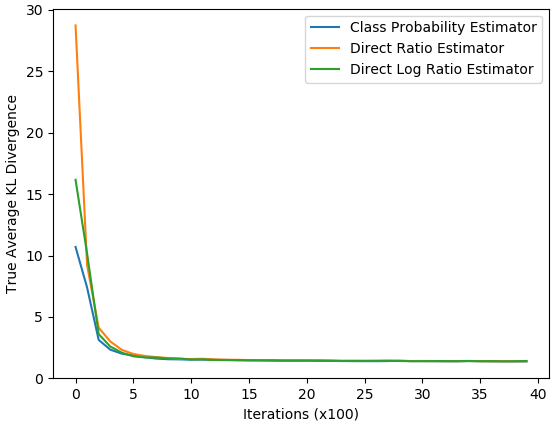
\includegraphics[width=\linewidth]{part2truklmins/JCKLDvsJCKLexpvsJCKLgudlog.png}
\caption{Reverse KL Divergence}
\end{subfigure}
\caption{\small Similar to the true KL divergence plots in Figure 7.2, these joint-contrastive plots show that the estimators formulated with the GAN divergence experience faster initial convergence. However, this is unreliable as the reverse KL divergence experiments appear to initialize at a much higher true KL divergence.}
\end{figure}
\begin{figure}[h]
\begin{subfigure}{0.49\textwidth}
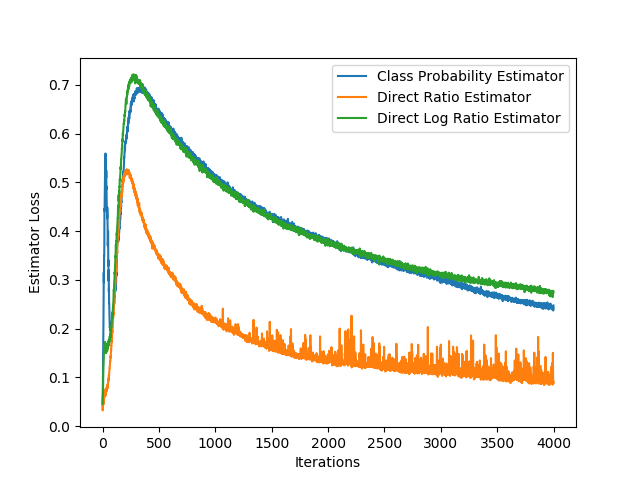
\includegraphics[width=\linewidth]{part2estimatorlosses/JCADVvsJCADVexpvsJCADVgudlog.png}
\caption{GAN Divergence}
\end{subfigure}
\begin{subfigure}{0.49\textwidth}
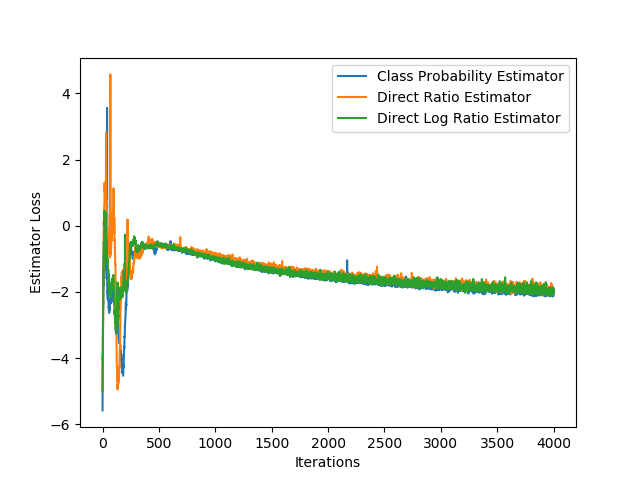
\includegraphics[width=\linewidth]{part2estimatorlosses/JCKLDvsJCKLexpvsJCKLgudlog.png}
\caption{Reverse KL Divergence}
\end{subfigure}
\caption{\small In these estimator loss plots, we again see that the reverse KL divergence plot demonstrates initial estimator instability. This is in stark contrast to the relatively stable GAN divergence plot. From sub-figure (a), we note that the direct ratio estimator is more unstable and has a lower loss value than the other two estimators. The cause of this is unknown, as the direct ratio estimator leads to similar posterior convergence to the more consistent class probability estimator.}
\end{figure}
\begin{figure}[h]
\begin{subfigure}{0.49\textwidth}
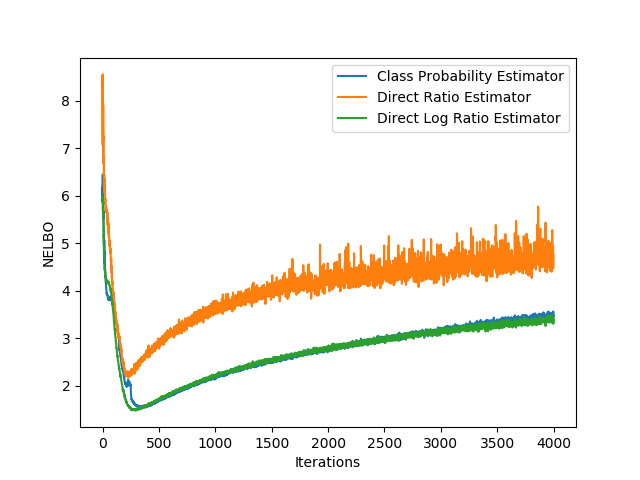
\includegraphics[width=\linewidth]{part2nelbos/JCADVvsJCADVexpvsJCADVgudlog.png}
\caption{GAN Divergence}
\end{subfigure}
\begin{subfigure}{0.49\textwidth}
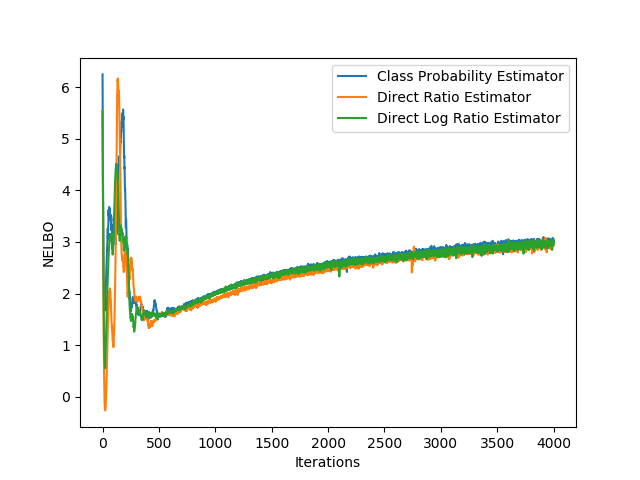
\includegraphics[width=\linewidth]{part2nelbos/JCKLDvsJCKLexpvsJCKLgudlog.png}
\caption{Reverse KL Divergence}
\end{subfigure}
\caption{\small The joint-contrastive estimated $NELBO$ plots above generally have similar trends to the corresponding estimator plots. Here we note that the final $NELBO$ value of the reverse KL divergence experiments is lower than that of the GAN divergence. However, this may be due to its initial fluctuations delaying the start of the increasing $NELBO$ trend by approximately 250 iterations.}
\end{figure}
\newpage
\chapter{Autoencoder Experiment - (MNIST Dataset)}\label{ch8}
In this chapter we compare the different $f$-divergence bounds and estimator parametrizations in the density ratio estimation involved with the autoencoder formulation. Specifically, we use the MNIST dataset: a popular dataset used in machine learning algorithms. Again, we undertrain the estimators to determine which parametrization performs the best. The primary goals of this experiment are to confirm the conclusions presented in \autoref{ch7}, and to gain further insights by applying the algorithms to a different experimental setting. Due to limited computational time, we only test the prior-contrastive algorithms. We repeat the experiment with two different latent spaces, one with 2 dimensions and one with 20 dimensions, to determine if the dimensionality of the densities has any effect on the results.
\section{Experiment Outline}
The MNIST (Modified National Institute of Standards and Technology) dataset is widely used for testing machine learning algorithms related to image analysis. It contains 60,000 labelled training images and 10,000 testing images of handwritten digits, each grayscale and of 28x28 pixel size. A sample of the images can be seen in \autoref{fig:8.1}. Our algorithms do not require the images to be labelled so we combine the two image sets and ignore the labelling.
\begin{figure}[b]
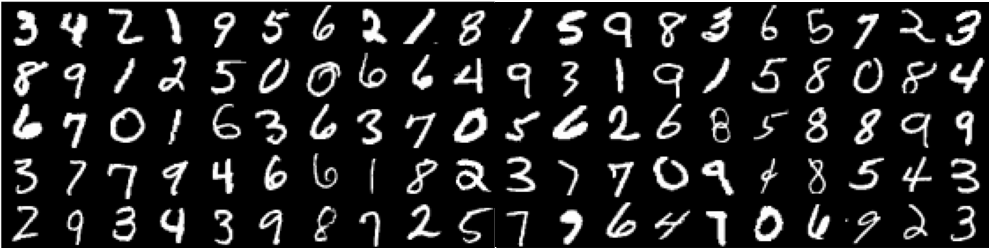
\includegraphics[width=\linewidth]{mnist-digits-small.png}
\caption{Samples from the MNIST Dataset}
\label{fig:8.1}
\end{figure}

In this problem, we train autoencoders on the MNIST dataset using various density ratio estimation algorithms. Specifically, we use the ``Adversarial Variational Bayes" variation of the autoencoder as described in \autoref{sec:3.8.1}. Recall that the associated optimization problem is:
\[\min_{\phi,\theta}\left\lbrace\E_{q^*(x)}\left[-\E_{q_\phi(z|x)}[\log p_\theta(x|z)]+KL(q_\phi(z|x)\|p(z))\right]\right\rbrace.\]
We therefore have three neural networks, illustrated in Figures 8.2\textendash 8.4. The notation in these figures is the same as in Figures 5.2 and 5.3, and the variational posterior and estimator networks have a relatively similar structure to the neural networks used in Chapters 6 and 7.
\begin{itemize}
\item An encoder network $\mathcal{G}_\phi(\varepsilon;x)$ that outputs samples from the variational posterior $q_\phi(z|x)$, effectively creating a latent representation of a data sample $x$.
\begin{figure}[h!]
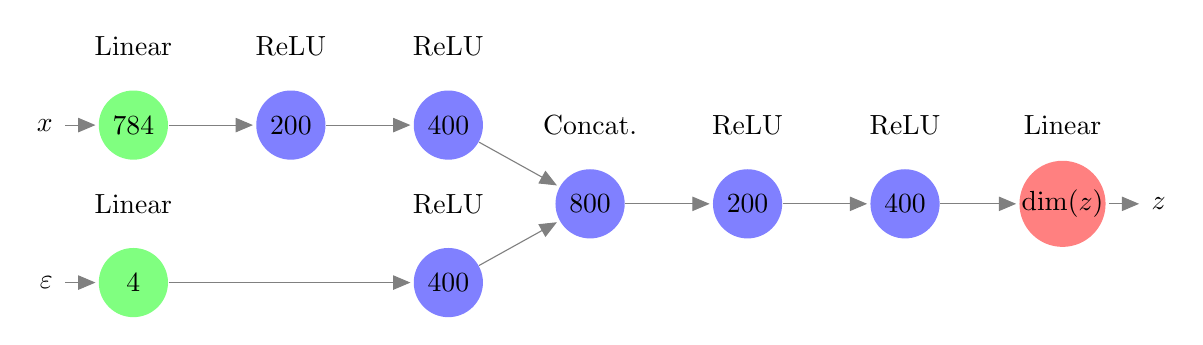
\begin{tikzpicture}[shorten >=1pt,->,draw=black!50, node distance=2.5cm]
    \tikzstyle{every pin edge}=[<-,shorten <=1pt]
    \tikzstyle{neuron}=[circle,fill=black!25,minimum size=25pt,inner sep=0pt]
    \tikzstyle{input neuron}=[neuron, fill=green!50];
    \tikzstyle{output neuron}=[neuron, fill=red!50];
    \tikzstyle{hidden neuron}=[neuron, fill=blue!50];
    \tikzstyle{annot} = [text width=4em, text centered]
    
	%\node[input neuron, pin=left:Bias] (I-0) at (0,0) {$x_0$};
    % Draw the input layer nodes
    %\foreach \name / \y in {1,...,3}
    % This is the same as writing \foreach \name / \y in {1/1,2/2,3/3,4/4}
    \node[input neuron, pin=left:$x$] (I-1) at (0,-1) {$784$};
	\node[input neuron, pin=left:$\varepsilon$] (I-2) at (0,-3) {$4$};

    \path[yshift=0cm] node[hidden neuron] (H-11) at (2.0cm,-1) {$200$};
	\path[yshift=0cm] node[hidden neuron] (H-12) at (4.0cm,-1) {$400$};
    \path[yshift=0cm] node[hidden neuron] (H-2) at (4.0cm,-3) {$400$};
    \path[yshift=0cm] node[hidden neuron] (H-3) at (5.8cm,-2) {$800$};
    \path[yshift=0cm] node[hidden neuron] (H-31) at (7.8cm,-2) {$200$};
    \path[yshift=0cm] node[hidden neuron] (H-32) at (9.8cm,-2) {$400$};
	\path[yshift=0cm] node[output neuron,pin={[pin edge={->}]right:$z$}] (O) at (11.8cm, -2) {dim$(z)$};
    \path (I-1) edge (H-11);
    \path (H-11) edge (H-12);
	\path (I-2) edge (H-2);
	\path (H-12) edge (H-3);
	\path (H-2) edge (H-3);
	\path (H-3) edge (H-31);
	\path (H-31) edge (H-32);
	\path (H-32) edge (O);
    % Annotate the layers
    \node[annot,above of=I-1, node distance=1cm] {Linear};
    \node[annot,above of=I-2, node distance=1cm] {Linear};
    \node[annot,above of=H-11, node distance=1cm] {ReLU};
    \node[annot,above of=H-12, node distance=1cm] {ReLU};
    \node[annot,above of=H-2, node distance=1cm] {ReLU};
    \node[annot,above of=H-3, node distance=1cm] {Concat.};
    \node[annot,above of=H-31, node distance=1cm] {ReLU};
    \node[annot,above of=H-32, node distance=1cm] {ReLU};
    \node[annot,above of=O, node distance=1cm] {Linear};
\end{tikzpicture}
\caption{\small This figure illustrates the structure of the generator network $\mathcal{G}(x,\bm{\varepsilon})$ used in the MNIST data generation experiment. The dimensionality of latent variable $z$ is either 2 or 20 depending on the experimental setting. We have arbitrarily chosen the number of random noise inputs $\varepsilon$ to be 4.}
\end{figure}
\item A decoder network representing the likelihood density $p_\theta(x|z)$ that reconstructs a data sample $x$ from a latent variable input $z$.
\begin{figure}[h!]
\centering
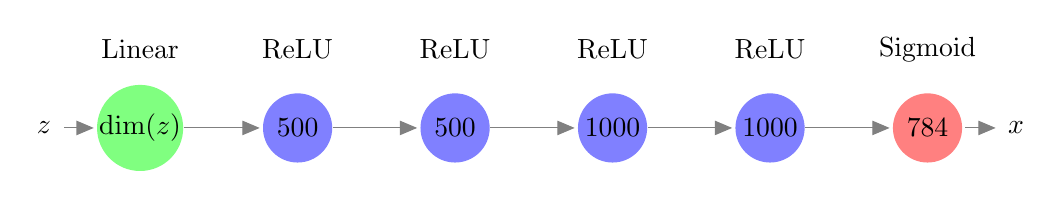
\begin{tikzpicture}[shorten >=1pt,->,draw=black!50, node distance=2.5cm]
    \tikzstyle{every pin edge}=[<-,shorten <=1pt]
    \tikzstyle{neuron}=[circle,fill=black!25,minimum size=25pt,inner sep=0pt]
    \tikzstyle{input neuron}=[neuron, fill=green!50];
    \tikzstyle{output neuron}=[neuron, fill=red!50];
    \tikzstyle{hidden neuron}=[neuron, fill=blue!50];
    \tikzstyle{annot} = [text width=4em, text centered]
    
	%\node[input neuron, pin=left:Bias] (I-0) at (0,0) {$x_0$};
    % Draw the input layer nodes
    %\foreach \name / \y in {1,...,3}
    % This is the same as writing \foreach \name / \y in {1/1,2/2,3/3,4/4}
    \node[input neuron, pin=left:$z$] (I-1) at (0,-1) {dim$(z)$};
    \path[yshift=0cm] node[hidden neuron] (H-1) at (2.0cm,-1) {$500$};
	\path[yshift=0cm] node[hidden neuron] (H-2) at (4.0cm,-1) {$500$};
	\path[yshift=0cm] node[hidden neuron] (H-3) at (6.0cm,-1) {$1000$};
	\path[yshift=0cm] node[hidden neuron] (H-4) at (8.0cm,-1) {$1000$};
	\path[yshift=0cm] node[output neuron,pin={[pin edge={->}]right:$x$}] (O) at (10.0cm, -1) {$784$};
    \path (I-1) edge (H-1);
    \path (H-1) edge (H-2);
	\path (H-2) edge (H-3);
	\path (H-3) edge (H-4);
	\path (H-4) edge (O);
    % Annotate the layers
    \node[annot,above of=I-1, node distance=1cm] {Linear};
    \node[annot,above of=H-1, node distance=1cm] {ReLU};
    \node[annot,above of=H-2, node distance=1cm] {ReLU};
    \node[annot,above of=H-3, node distance=1cm] {ReLU};
    \node[annot,above of=H-4, node distance=1cm] {ReLU};
    \node[annot,above of=O, node distance=1cm] {Sigmoid};
\end{tikzpicture}
\caption{\small This is a diagram of the decoder network used in the MNIST data generation experiment. A sigmoid output layer is used to map the network output to $(0,1)$, suiting the grayscale nature of the data. Although this problem involves image analysis, we refrain from using convolutional layers due to the relatively small image size. This is consistent with other similar MNIST experiments \citep{nowozin, bgan}.}
\end{figure}
\item A density ratio estimator network ($D_\alpha(z,x),r_\alpha(z,x)$ or $T_\alpha(z,x)$) used to evaluate the intractable $KL(q_\phi(z|x)\|p(z))$ term in the optimization problem.
\begin{figure}[h!]
\centering
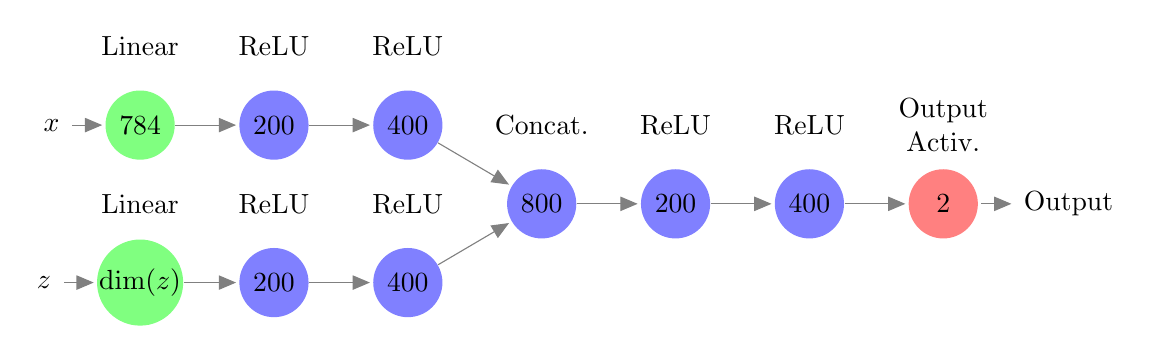
\begin{tikzpicture}[shorten >=1pt,->,draw=black!50, node distance=2.5cm]
    \tikzstyle{every pin edge}=[<-,shorten <=1pt]
    \tikzstyle{neuron}=[circle,fill=black!25,minimum size=25pt,inner sep=0pt]
    \tikzstyle{input neuron}=[neuron, fill=green!50];
    \tikzstyle{output neuron}=[neuron, fill=red!50];
    \tikzstyle{hidden neuron}=[neuron, fill=blue!50];
    \tikzstyle{annot} = [text width=4em, text centered]
    
	%\node[input neuron, pin=left:Bias] (I-0) at (0,0) {$x_0$};
    % Draw the input layer nodes
    %\foreach \name / \y in {1,...,3}
    % This is the same as writing \foreach \name / \y in {1/1,2/2,3/3,4/4}
    \node[input neuron, pin=left:$x$] (I-1) at (0,-1) {$784$};
	\node[input neuron, pin=left:$z$] (I-2) at (0,-3) {dim$(z)$};

    \path[yshift=0cm] node[hidden neuron] (H-11) at (1.7cm,-1) {$200$};
	\path[yshift=0cm] node[hidden neuron] (H-12) at (3.4cm,-1) {$400$};
	\path[yshift=0cm] node[hidden neuron] (H-21) at (1.7cm,-3) {$200$};
    \path[yshift=0cm] node[hidden neuron] (H-22) at (3.4cm,-3) {$400$};
    \path[yshift=0cm] node[hidden neuron] (H-3) at (5.1cm,-2) {$800$};
    \path[yshift=0cm] node[hidden neuron] (H-31) at (6.8cm,-2) {$200$};
    \path[yshift=0cm] node[hidden neuron] (H-32) at (8.5cm,-2) {$400$};
	\path[yshift=0cm] node[output neuron,pin={[pin edge={->}]right:Output}] (O) at (10.2cm, -2) {$2$};
    \path (I-1) edge (H-11);
    \path (H-11) edge (H-12);
	\path (I-2) edge (H-21);
	\path (H-21) edge (H-22);
	\path (H-12) edge (H-3);
	\path (H-22) edge (H-3);
	\path (H-3) edge (H-31);
	\path (H-31) edge (H-32);
	\path (H-32) edge (O);
    % Annotate the layers
    \node[annot,above of=I-1, node distance=1cm] {Linear};
    \node[annot,above of=I-2, node distance=1cm] {Linear};
    \node[annot,above of=H-11, node distance=1cm] {ReLU};
    \node[annot,above of=H-12, node distance=1cm] {ReLU};
    \node[annot,above of=H-21, node distance=1cm] {ReLU};
    \node[annot,above of=H-22, node distance=1cm] {ReLU};
    \node[annot,above of=H-3, node distance=1cm] {Concat.};
    \node[annot,above of=H-31, node distance=1cm] {ReLU};
    \node[annot,above of=H-32, node distance=1cm] {ReLU};
    \node[annot,above of=O, node distance=1cm] {Output Activ.};
\end{tikzpicture}
\caption{\small This figure depicts the estimator network for the MNIST data generation experiment. Depending on the estimator parametrization, the output activation function is either sigmoid for the class probability estimator $D_\alpha(z,x)\simeq q_\phi(z|x)/(q_\phi(z|x)+p(z))$, exponential for the direct ratio estimator $r_\alpha(z,x)\simeq q_\phi(z|x)/p(z)$ or linear for the direct log ratio estimator $T_\alpha(z,x)\simeq \log (q_\phi(z|x)/p(z))$.}
\end{figure}
\end{itemize}
The program alternates between multiple iterations of estimator training and a single, simultaneous training step of the encoder and decoder weights.

Unlike the ``Adversarial Variational Bayes" specification in \autoref{sec:3.8.1}, we do not input random noise to the decoder, therefore resulting in a deterministic output. This is depicted in Figure 8.5. To express the likelihood term $\E_{q_\phi(z|x)}[\log p_\theta(x|z)]$ in the optimization problem, we use the likelihood function of a Bernoulli density, with probability equal to the output of the decoder. This likelihood representation is common in literature, and is used for several reasons \citep{nowozin,bgan, tiao}:
\begin{itemize}
\item Image blurriness is reduced as there is no random noise in the pixel values.
\item We use the reconstruction error $\|x-\tilde{x}\|^2$ to evaluate convergence, so a noisy sample reconstruction can make it difficult to compare the algorithms.
\item In this experiment, we are primarily interested in the accuracy of the density ratio estimation between the variational posterior and the prior: this is independent of the decoder parametrization.
\end{itemize}
We avoid using kernel density estimation to evaluate convergence as it is inaccurate in high dimensions.
\begin{figure}[h]
  \centering
  \tikz{ %
    \node[latent] (x) {$x$} ; %
    \node[det, right=of x] (q) {$\mathcal{G}_\phi(\varepsilon_1;x)$} ; %
    \node [latent, above=of q] (eps) {$\varepsilon_1$} ;
    \node [latent, right=of q] (z) {$z$} ;
    \node [det, right=of z] (p) {$p_\theta(x|z)$} ;
    \node [latent, right=of p] (pout) {$\tilde{x}$} ;
    \edge {x} {q} ; %
    \edge {q} {z}
    \edge {eps} {q} ;
    \edge {z} {p} ;
    \edge {p} {pout} ;
  }
   \caption{\small This diagram depicts the ``Adversarial Variational Bayes" formulation of the variational autoencoder used in the MNIST data generation experiment. Note that there is no random noise added to the decoder.}
\end{figure}

Our experiment parameters have been configured to be similar to the MNIST experiment performed in ``$f$-GAN: Training Generative Neural Samplers using Variational Divergence Minimization" by \citet{nowozin}: a large batch size of 2048 is used, and for each network, a training rate of 0.0004 is used in the low dimensional configuration, whilst the high dimensional setting uses a training rate of 0.0001. Again, the estimator is pre-trained for 5000 iterations, afterwards the program alternates between 20 iterations of estimator optimizaton and 1 iteration of posterior training, for 4000 total posterior iterations. \autoref{alg:mnist} in \autoref{app:B.4} depicts pseudocode for this experiment. Like in the ``Sprinkler" experiments, the estimator loss and estimated $NELBO$ at each posterior iteration was saved, and every 10 posterior iterations, 500 MNIST samples were passed through the autoencoder and the average reconstruction error $\|x-\tilde{x}\|^2$ was saved.
\section{Low Dimensional Experiment Results}
Table 8.1 below tabulates the mean and standard deviation of the autoencoder's final reconstruction error between the 30 experiment repetitions. Figures 8.6 depicts a visual representation of these values. As reflected in Figures 8.7\textendash 8.9, most of the distinctions are relatively minor, likely because the estimators experience a higher level of training in comparison to the experiment in \autoref{ch7}. Additionally, the presence of the likelihood term in the $NELBO$ loss function reduces the importance of accurate density ratio estimation. In this experiment, the most notable observation is that the direct log ratio estimator trained with a GAN divergence leads to substantially higher reconstruction error.  
\begin{table}[h]
\centering
\begin{tabular}{|l|c|c|c|}
\hline
\multicolumn{4}{|c|}{Prior-Contrastive Results}\\
\hline
\multicolumn{2}{|c|}{Algorithm} & Mean Reconstruction Error & Standard Deviation\\
\hline
\multirow{3}{*}{Reverse KL} & $D_\alpha(z,x)$ & \textbf{0.08662} & 0.00154\\
\cline{2-4}
& $r_\alpha(z,x)$ & 0.08710 & 0.00214\\
\cline{2-4}
& $T_\alpha(z,x)$ & 0.08730 & 0.00157\\
\hline
\multirow{3}{*}{GAN} & $D_\alpha(z,x)$ & 0.08673 & \textbf{0.00129}\\
\cline{2-4}
& $r_\alpha(z,x)$ & 0.08716 & 0.00151\\
\cline{2-4}
& $T_\alpha(z,x)$ & 0.10683 & 0.00199\\
\hline
\end{tabular}
\caption{\small The low-dimensional MNIST autoencoder experiment results are tabulated above. We note that the relative performances of the different estimator loss functions is the same as in \autoref{ch7}.}
\end{table}
\begin{figure}[h!]
\begin{subfigure}{\textwidth}
\centering
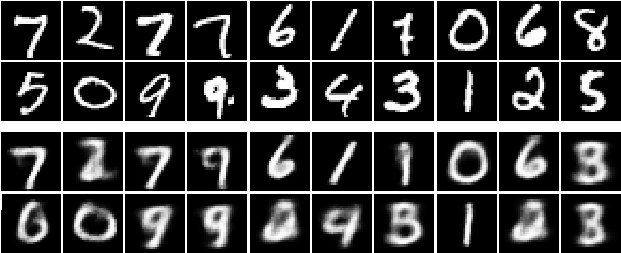
\includegraphics[width=0.9\linewidth]{086729.png}
\caption{Reconstruction Error of 0.08673}
\end{subfigure}
\begin{subfigure}{\textwidth}
\centering
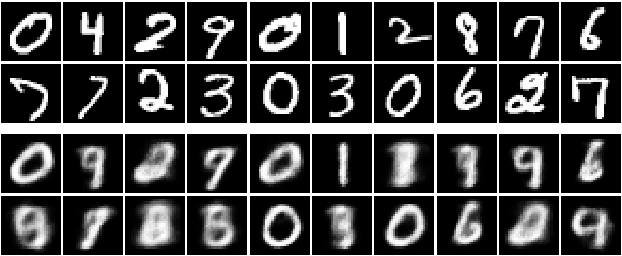
\includegraphics[width=0.9\linewidth]{105329.png}
\caption{Reconstruction Error of 0.10533}
\end{subfigure}
\caption{\small These figures exemplify data reconstruction corresponding to different reconstruction errors. The first two rows of each sub-figure depict example data input $x$, and the last two rows show the reconstructed output $\tilde{x}$.}
\end{figure}
\begin{figure}[h!]
\centering
\begin{subfigure}{0.49\textwidth}
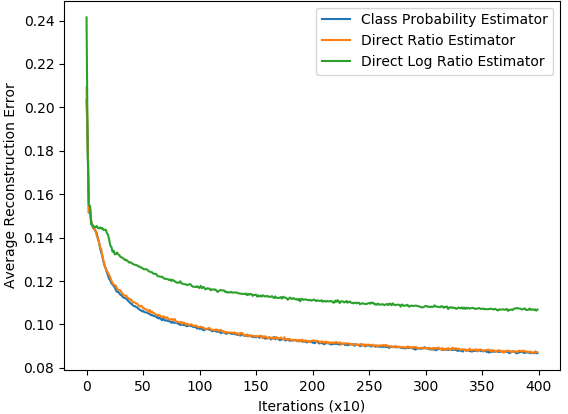
\includegraphics[width=\linewidth]{part3reconerrors/PCADVvsPCADVexpvsPCADVgudlog.png}
\caption{GAN Divergence}
\end{subfigure}
\begin{subfigure}{0.49\textwidth}
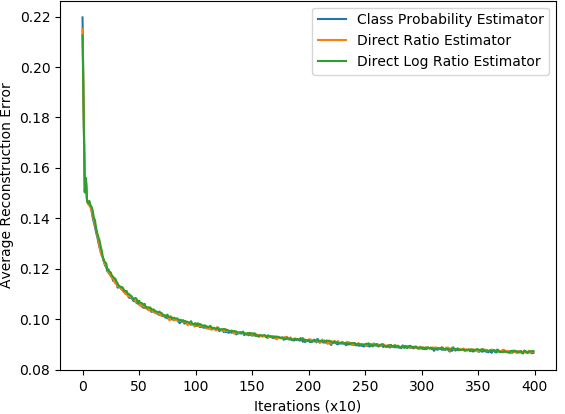
\includegraphics[width=\linewidth]{part3reconerrors/PCKLDvsPCKLexpvsPCKLgudlog.png}
\caption{Reverse KL Divergence}
\end{subfigure}
\caption{\small As shown in the above average reconstruction error plots, the direct log ratio estimator in sub-figure (a) consistently has a higher reconstruction error.}
\end{figure}

\begin{figure}[h!]
\centering
\begin{subfigure}{0.49\textwidth}
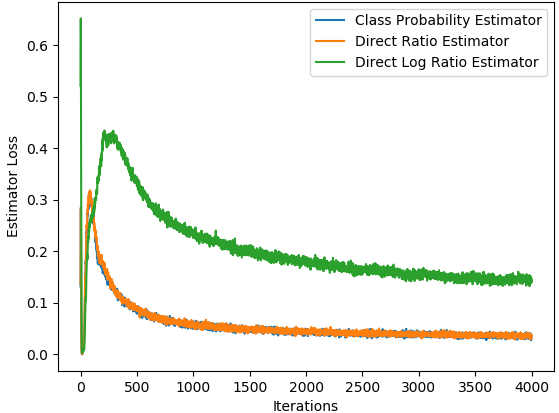
\includegraphics[width=\linewidth]{part3estimatorlosses/PCADVvsPCADVexpvsPCADVgudlog.png}
\caption{GAN Divergence}
\end{subfigure}
\begin{subfigure}{0.49\textwidth}
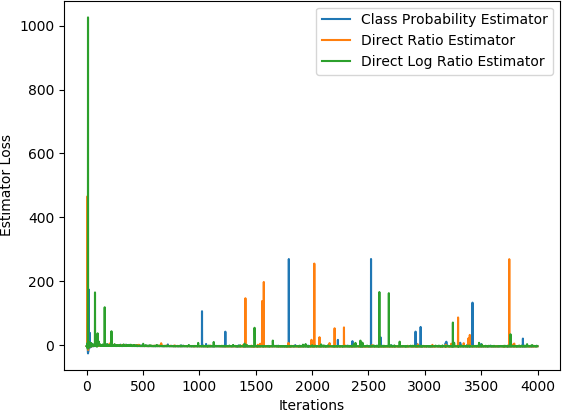
\includegraphics[width=\linewidth]{part3estimatorlosses/PCKLDvsPCKLexpvsPCKLgudlog.png}
\caption{Reverse KL Divergence}
\end{subfigure}
\caption{\small Noting the scale of the estimator loss plot in sub-figure (b), it is evident that the reverse KL divergence leads to unstable estimator training. Unlike the estimators plotted in Figure 7.3 (b), these estimators don't appear to stabilize after a certain period. Sub-figure (a) shows that the direct log ratio estimator loss is consistently higher than the other two estimators, correlating with its poorer reconstruction.}
\end{figure}
\begin{figure}[h!]
\centering
\begin{subfigure}{0.49\textwidth}
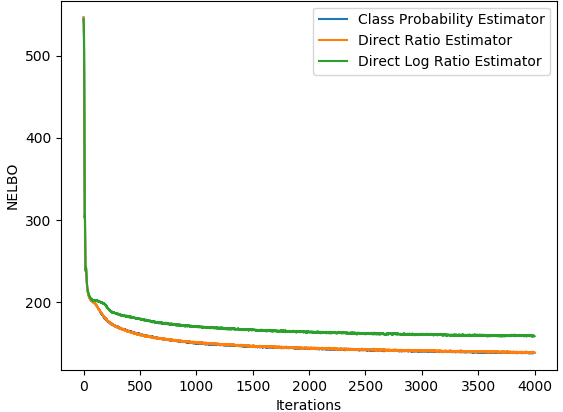
\includegraphics[width=\linewidth]{part3nelbos/PCADVvsPCADVexpvsPCADVgudlog.png}
\caption{GAN Divergence}
\end{subfigure}
\begin{subfigure}{0.49\textwidth}
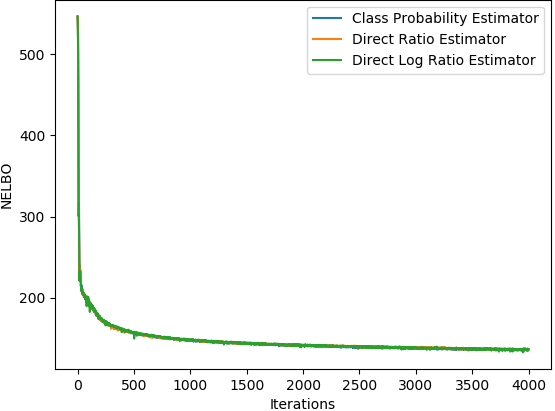
\includegraphics[width=\linewidth]{part3nelbos/PCKLDvsPCKLexpvsPCKLgudlog.png}
\caption{Reverse KL Divergence}
\end{subfigure}
\caption{\small Despite the apparent instability of the estimators trained with the reverse KL divergence, the $NELBO$ plot in sub-figure (b) is relatively consistent, leading to a smooth convergence as plotted in Figure 8.7 (b). The high direct log ratio estimator loss associated with the GAN divergence corresponds to a relatively large $NELBO$, as depicted in sub-figure (a).}
\end{figure}
\newpage
\section{High Dimensional Experiment Results}
When the dimensionality of the latent space was increased to 20, the direct ratio and log ratio estimator loss functions involved quantities greater than the largest representable 64-bit floating point number, overflowing to \verb+Inf+ and outputting \verb+NaN+ for the remainder of the program runtime. This is because the density ratio $q_\phi(z|x)/p(z)$ increases with the dimensionality of the latent space, eventually reaching a value too large to be represented by a 64-bit float. The direct ratio estimator $r_\alpha(z,x)\simeq q_\phi(z|x)/p(z)$ therefore fails in this scenario. This is consistent with the results in ``Generative Adversarial Nets from a Density Ratio Estimation Perspective" by \citet{bgan}. Now recall that the direct log ratio estimator loss function involves taking the exponential of the estimator output. For example, the loss function formulated by the reverse KL divergence is
\[-\E_{q^*(x)\pi(\varepsilon)}[T_\alpha(\mathcal{G}(\varepsilon;x),x)]+\E_{p(z)q^*(x)}[\exp(T_\alpha(z,x))].\]
So despite $T_\alpha(z,x)$ outputting the log of the density ratio, the exact density ratio is expressed in the loss function when the exponential is taken, causing the program to fail. On the other hand, the class probability estimator does not experience this problem as its output is bound in $(0,1)$.
\begin{lemma}
In the prior-contrastive setting, the output of the class probability estimator network before passing through the sigmoid activation function $g(x)=(1+e^{-x})^{-1}$ is the estimated log density ratio $\log \left(q_\phi(z|x)/p(z)\right)$. A similar result holds in the joint-contrastive setting.
\begin{proof}
Proof of this lemma can be found in \autoref{app:A.5}.
\end{proof}
\end{lemma}
\begin{remark}
The calculations with the class probability estimator $D_\alpha(z,x)$ involve values that lie within a larger bound of floating point representations than the values concerned with the direct ratio $r_\alpha(z,x)$ and log ratio $T_\alpha(z,x)$ estimators.
\end{remark}
We can therefore conclude that the class probability estimator is superior in the sense that it is the only feasible parametrization. It remains to compare the $f$-divergence used to formulate the estimator loss function. The reconstruction errors are tabulated in Table 8.2, and a visual representation of the errors is found in Figure 8.10. We notice that unlike our previous experimental results, the reverse KL divergence correlates to inferior results; this is reflected in the instability of its estimator throughout the program runtime, as shown in Figures 8.11\textendash 8.13. This contrasts with the results in \autoref{ch7}, where the estimators formulated by the reverse KL divergence experienced initial instability, but have more accurate density ratio estimation when stable. It is likely that the lack of estimator stabilization in this experiment occurs from the increased complexity of the MNIST dataset.  
\begin{table}[h]
\centering
\begin{tabular}{|c|c|c|}
\hline
\multicolumn{3}{|c|}{Prior-Contrastive Results}\\
\hline
Algorithm & Mean Reconstruction Error & Standard Deviation\\
\hline
Reverse KL - $D_\alpha(z,x)$ & 0.06470 & 0.01949\\
\hline
GAN - $D_\alpha(z,x)$ & \textbf{0.04440} & \textbf{0.00174}\\
\hline
\end{tabular}
\caption{\small In the high dimensional MNIST autoencoder experiment results, it is evident that the GAN divergence correlates with substantially lower reconstruction error mean and standard deviation, contradicting the superiority of the reverse KL divergence shown in previous experiments.}
\end{table}
\begin{figure}[h!]
\begin{subfigure}{\textwidth}
\centering
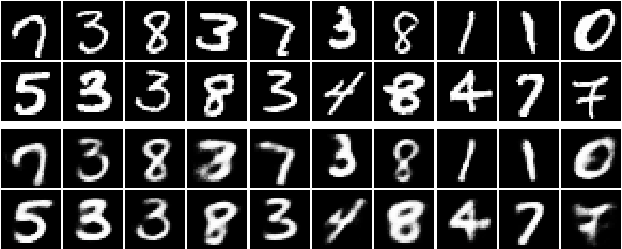
\includegraphics[width=0.9\linewidth]{044944.png}
\caption{Reconstruction Error of 0.04494}
\end{subfigure}
\begin{subfigure}{\textwidth}
\centering
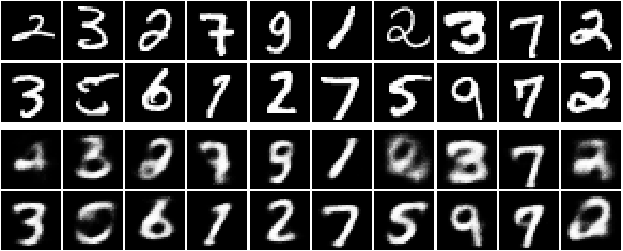
\includegraphics[width=0.9\linewidth]{064834.png}
\caption{Reconstruction Error of 0.064834}
\end{subfigure}
\caption{\small Similar to Figure 8.6, these figures exemplify data reconstruction corresponding to different reconstruction errors.}
\end{figure}
\begin{figure}[h]
\centering
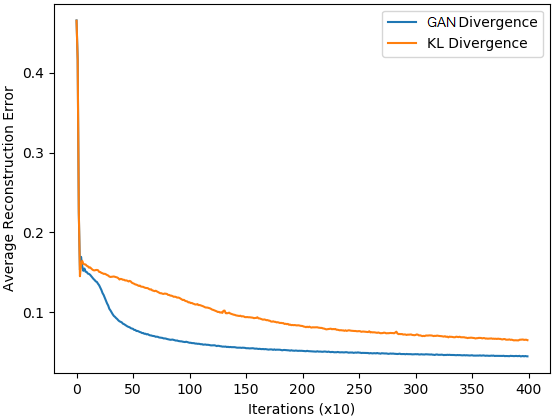
\includegraphics[width=0.49\linewidth]{part4reconerrors/PCADVvsPCKLD.png}
\caption{\small This plot shows that the reconstruction error associated with the reverse KL divergence is consistently higher for the majority of the program runtime.}
\end{figure}
\begin{figure}[h]
\centering
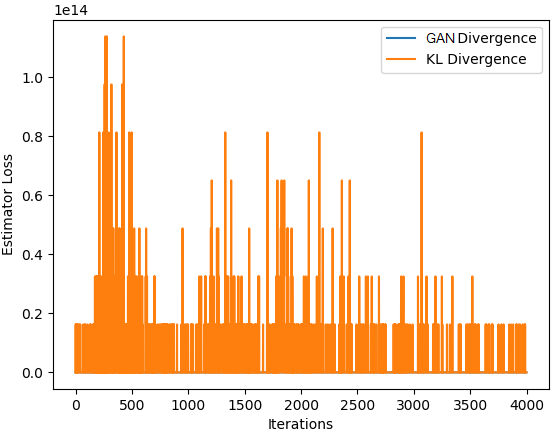
\includegraphics[width=0.49\linewidth]{part4estimatorlosses/PCADVvsPCKLD.png}
\caption{\small The estimator loss corresponding to the reverse KL divergence appears to be extremely unstable for the entire program runtime, spiking to values exceeding $10^{14}$. On the other hand, the GAN divergence estimator loss appears to be relatively stable.}
\end{figure}
\begin{figure}[h]
\centering
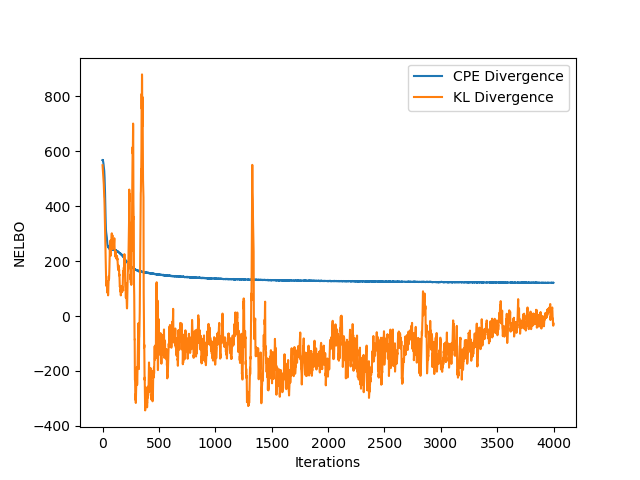
\includegraphics[width=0.49\linewidth]{part4nelbos/PCADVvsPCKLD.png}
\caption{\small The instability of the reverse KL divergence estimator loss propagates to its $NELBO$ estimation, which appears to fluctuate wildly. This correlates to the superiority of the GAN divergence in this particular experiment. It appears that the reverse KL estimator in this experiment has not stabilized, leading to poorer network convergence.}
\end{figure}
\chapter{Conclusion and Further Research}\label{ch9}
In this thesis, we have compared various density ratio estimator loss functions in both prior-contrastive and joint-contrastive contexts for a simple Bayesian posterior inference problem, and in the prior-contrastive context for an autoencoder trained on the MNIST dataset. In \autoref{ch5}, we generalized the estimator loss function specification to the choice of $f$-divergence and estimator parametrization. To the best of our knowledge, this generalization has not yet been presented in the current literature and can be used to gain further insights into these loss functions. Applying this framework, we showed in Chapters \ref{ch6} and \ref{ch7} that the different estimator parametrizations have similar accuracies when optimally trained, but when under-trained, higher posterior convergence is correlated with faster estimator convergence, exhibited by the class probability estimator. These chapters also demonstrated that estimators trained with the reverse KL divergence may be initially unstable, particularly when undertrained, but demonstrate high density ratio estimation accuracy when stable. On the other hand, estimators trained with the GAN divergence are relatively stable but lead to lower posterior convergence. These results were verified in the MNIST autoencoder experiment discussed in \autoref{ch8}. This cemented the class probability estimator as the superior estimator parametrization, as the values associated with the direct ratio and direct log ratio estimators were too large to be efficiently stored in a digital representation. We believe these results are unique contributions to the field.
\section{Further Research}
In this thesis, we have only compared the use of the reverse KL divergence and the GAN divergence in formulating the estimator loss function. ``$f$-GAN: Training Generative Neural Samplers using Variational Divergence Minimization" by \citet{nowozin} compares several different $f$-divergences such as the Pearson divergence and the forward KL divergence, but only assesses the posterior convergence. An analysis on the estimator losses and estimated $NELBO$s over the program runtime may reveal insights on the tradeoff between estimator stability and accuracy. Nowozin's paper also uses different estimator parametrizations for each $f$-divergence; comparing the $f$-divergences with the same class probability estimator parametrization may lead to more reliable results.

There are alternative estimator parametrizations to test. For example, to alleviate the issues associated with an excessively high density ratio, ``Generative Adversarial Nets from a Density Ratio Estimation Perspective" by \citet{bgan} proposes that the direct density ratio estimator be parametrized as $r_\alpha(u)\simeq q(u)/(\beta q(u)+(1-\beta)p(u))$ where $\beta>0$ is small.

In our experiments, we have excluded the joint-contrastive autoencoder formulation, as described in ``Adversarially Learned Inference" by \citet{ali} due to lack of computational time, but comparing the estimators in this context may present new insights.

There are alternate methods of estimating the intractable KL divergence term in the $NELBO$ that do not involve Theorem \ref{4.2.1}. ``Divergence Estimation for Multidimensional Densities via $k$-Nearest-Neighbor Distances" by \citet{wang} describes a non-parametric method of estimating the KL divergence between two high dimensional densities. Rather than estimate the density ratio directly, a denoiser estimates the gradient of the log density, which can be used to minimize the KL divergence term in the $NELBO$ \citep{vincent}. These methods can be used to formulate new variational inference algorithms, and their performances can be compared with the algorithms discussed in this thesis.

Posterior convergence in our autoencoder experiment can be assessed more effectively by using Annealed Importance Sampling (AIS) to estimate the negative of the marginal density $-p(x)$, which can be compared with the estimated $NELBO$ which attains its minimum at that value. This process is detailed in ``On the Quantitative Analysis of Decoder-Based Generative Models" by \citet{ais}.


%%%%%%%%%%%%%%%%%%%%%%%%%%%%%%%%%%%%%%%%%%%%%%%%%%%%%%%%%%%%%%%%%%%%%%%%%%
\clearpage
\addcontentsline{toc}{chapter}{References}
\bibliographystyle{apalike}
\bibliography{bible}



\newpage
\appendix
\chapter{Proofs}\label{app:A}
\section{Proof of Proposition 2.6.2}\label{app:A.1}
First we show that
\[\frac{{\rm d}}{{\rm d}\alpha}f\left(\bm{x}^{(n)}+\alpha \bm{s}^{(n)}\right)=\nabla f\left(\bm{x}^{(n)}+\alpha \bm{s}^{(n)}\right)^\top \bm{s}^{(n)},\]
where $\bm{x}^{(n)}=\left[x_1^{(n)},\dots,x_k^{(n)}\right]^\top$ and $\bm{s}^{(k)}=\left[s_1^{(n)},\dots,s_k^{(n)}\right]^\top$.\\
Let
\[x_i^{(n)}(\alpha)=x_i^{(n)}+\alpha s_i^{(n)},\quad i=1,\dots,n,\]
so that $\bm{x}^{(n)}+\alpha \bm{s}^{(n)}=\left[x_1^{(n)}(\alpha),\dots,x_k^{(n)}(\alpha)\right]^\top$.
We have
\begin{align*}
\frac{{\rm d}}{{\rm d}\alpha}f\left(\bm{x}^{(n)}+\alpha\bm{s}^{(n)}\right)&= \frac{{\rm d}}{{\rm d}\alpha}f\left(x_1^{(n)},\dots,x_k^{(n)}(\alpha)\right)\\
&= \sum^k_{i=1}\frac{\partial f(\bm{x})}{\partial x_i}|_{\bm{x}=\bm{x}^{(n)}+\alpha \bm{s}^{(n)}}\frac{{\rm d}\left(x_i^{(n)}(\alpha)\right)}{{\rm d}\alpha}\\
&=\sum_{i=1}^k\frac{\partial f(\bm{x})}{\partial x_i}|_{\bm{x}=\bm{x}^{(n)}+\alpha \bm{s}^{(n)}}\bm{s}_i^{(n)}\\
%\frac{\partial f(\bm{x})}{\partial x_1}|_{\bm{x}=\bm{x}^{(n)}+\alpha \bm{s}^{(n)}}\bm{s}_1^{(n)}+\dots+\frac{\partial f(\bm{x})}{\partial x_n}|_{\bm{x}=\bm{x}^{(n)}+\alpha \bm{s}^{(n)}}\bm{s}_k^{(n)}\\
&=\nabla f\left(\bm{x}^{(n)}+\alpha \bm{s}^{(n)}\right)^\top \bm{s}^{(n)}.
\end{align*}
Setting $\alpha=0$ and using Definition 2.7.1,
\[\frac{{\rm d}}{{\rm d}\alpha}f\left(\bm{x}^{(n)}+\alpha\bm{s}^{(n)}\right)|_{\alpha=0}=\nabla f\left(\bm{x}^{(n)}\right)^\top \bm{s}^{(n)}<0.\]
Therefore for sufficiently small $\alpha>0$,
\[f\left(x^{(n)}+\alpha s^{(n)}\right)<f\left(x^{(n)}\right).\]
\section{Proof of Lemma 3.2.4}\label{app:swag}
\begin{align*}
D_{RKL}(p(x)\|q(x))&=\mathbb{E}_{p(x)}\left[\frac{q(x)}{p(x)}\log \left(\frac{q(x)}{p(x)}\right)\right]\\
&=\int_\R p(x)\frac{q(x)}{p(x)}\log\left(\frac{q(x)}{p(x)}\right)\, {\rm d}x\\
&= \int_\R q(x)\log\left(\frac{q(x)}{p(x)}\right)\, {\rm d}x\\
&= \mathbb{E}_{q(x)}\left[\log \left(\frac{q(x)}{p(x)}\right)\right]\\
&=KL(q(x)\|p(x)).
\end{align*}
\section{Proof of Lemma 3.2.5}\label{app:asdf}
We prove this in the case where $p(x)$ and $q(x)$ are continuous densities: a similar proof holds when they are discrete.
\begin{align*}
KL(p(x)\|q(x))&=\int_\R p(x)\log \left(\frac{p(x)}{q(x)}\right)\, {\rm d}x\\
&=-\int_\R p(x)\log \left(\frac{q(x)}{p(x)}\right)\, {\rm d}x\\
&\geq -\int_\R p(x) \left(\frac{q(x)}{p(x)}-1\right)\, {\rm d}x\\
&=-\int_\R q(x)dx + \int_\R p(x)\, {\rm d}x\\
&=0.
\end{align*}
In the third line we use $-\log x \geq -(x-1)$ for all $x>0$ with equality if and only if $x=1$, therefore $KL(q(x)\|p(x))=0$ if and only if $q(x)=p(x)$. The last line is due to $p(x)$ and $q(x)$ being probability densities.
\section{Proof of Lemma 3.7.1}\label{app:A.2}
Denoting the identity matrix as $I$ and the covariance matrix of $q_\phi(\bm{z}|\bm{x})$ as $\Sigma$, we state the probability density functions of the two densities:
\[q_\phi(\bm{z}|\bm{x})=\frac{1}{(2\pi)^{M/2}\det(\Sigma)^{1/2}}\exp\left(-\frac{1}{2}(\bm{z}-\bm{\mu})^\top\Sigma^{-1}(\bm{z}-\bm{\mu})\right),\]
\[p(\bm{z})=\frac{1}{(2\pi)^{M/2}}\exp\left(-\frac{1}{2}\bm{z}^\top I\bm{z}\right).\]
From Definition 3.2.2, we have:
\begin{align*}
KL(q_\phi(\bm{z}|\bm{x})\|p(\bm{z}))&=\E_{q_\phi(\bm{z}|\bm{x})}[\log q_\phi(\bm{z}|\bm{x})-\log p(\bm{z})]\\
&=-\frac{1}{2}\log(\det \Sigma)+\frac{1}{2}\E_{q_\phi(\bm{z}|\bm{x})}\left[-(\bm{z}-\bm{\mu})^\top \Sigma^{-1}(\bm{z}-\bm{\mu})+\bm{z}^\top I\bm{z}\right]\\
&=-\frac{1}{2}\log(\det \Sigma)+\frac{1}{2}\E_{q_\phi(\bm{z}|\bm{x})}\left[-\tr\left(\Sigma^{-1}\Sigma\right)+\tr\left(I\bm{z}\bm{z}^\top\right)\right]\\
&=-\frac{1}{2}\log(\det \Sigma)-\frac{M}{2}+\frac{1}{2}\tr\left(I+\left(\Sigma+\mu\mu^\top\right)\right)\\
&=\frac12 \sum_{i=1}^M\left(\sigma^2_i+\mu^2_i-\log(\sigma^2_i)-1\right).
\end{align*}
\section{Proof of Lemma 4.1.1}\label{app:A.3}
First we write the discriminator loss function in integral form:
\[L_D=-\int_U q(u)\log D_\alpha(u)\, {\rm d}u-\int_U p(u)\log(1-D_\alpha(u))\, {\rm d}u.\]
Now we take the functional derivative of the expression and equate it to $0$:
\[\frac{\partial L_D}{\partial D_\alpha(u)}=0\]
\[-\frac{q(u)}{D_\alpha(u)}+\frac{p(u)}{1-D_\alpha(u)}=0\]
%\[p(u)D_\alpha(u)-q(u)(1-D_\alpha(u))=0\]
\[D_\alpha(u)(q(u)+p(u))=q(u)\]
\[D_\alpha(u)=\frac{q(u)}{q(u)+p(u)}.\]
Observing that $q(u)$ and $p(u)$ are densities, this expression is a minimum as
\begin{align*}
\frac{\partial^2L_D}{\partial D^2_\alpha(u)}&=\frac{q(u)}{D^2_\alpha(u)}+\frac{p(u)}{(1-D_\alpha(u))^2}\\
&>0.
\end{align*}
It can be shown that the conditions to take the first and second functional derivative using the Euler-Lagrange equation are met.
\section{Proof of Lemma 4.2.2}\label{app:A.4}
First we write the ratio loss function in integral form:
\[L_r=-\int_U q(u)\log r_\alpha(u)\, {\rm d}u+\int_U p(u)r_\alpha(u)\, {\rm d}u.\]
Now we take the functional derivative of the expression and equate it to 0:
\[\frac{\partial L_r}{\partial r_\alpha(u)}=0\]
\[-\frac{q(u)}{r_\alpha (u)}+p(u)=0\]
\[r_\alpha(u)=\frac{q(u)}{p(u)}.\]
Observing that $q(u)$ is a density, this expression is a minimum as:
\begin{align*}
\frac{\partial^2L_r}{\partial r_\alpha^2(u)}&=\frac{q(u)}{r_\alpha^2(u)}\\
&>0.
\end{align*}
\section{Proof of Lemma 8.3.1}\label{app:A.5}
Letting $x$ be the neural network output before being mapped to $(0,1)$, we have:
\begin{align*}
\frac{1}{1+e^{-x}}&\simeq\frac{q_\phi(z|x)}{p(z)+q_\phi(z|x)}\\
e^{-x}+1&\simeq\frac{p(z)+q_\phi(z|x)}{q_\phi(z|x)}\\
e^{-x}&\simeq\frac{p(z)}{q_\phi(z|x)}\\
x&\simeq\log \frac{q_\phi(z|x)}{p(z)}.
\end{align*}
\chapter{Algorithms}\label{app:B}
\section{Back-Propagation Algorithm}\label{app:B.1}
\begin{algorithm}
\caption{Back-Propagation Algorithm}
\KwData{Training Data $\{(\bm{x}^{(1)},\bm{y}^{(1)}),\dots ,(\bm{x}^{(N)},\bm{y}^{(N)})\}$}
\KwResult{Cost Function Partial Derivatives $\frac{\partial}{\partial\Theta^{(j)}_{m,n}}L(\Theta)$}
\BlankLine
\Begin{Initialize weights $\Theta$ using Xavier Initialization\;
Set $\Delta^{(j)}_{m,n}=0 \quad \forall j,m,n$\;
\For{$I=1$ \KwTo $N$}{
Set $\bm{a}^{(1)}=\bm{x}^{(I)}$\;
\For{$j=2$ \KwTo $J$}{
Set $\bm{a}^{(j)}=\Theta^{(j-1)^\top}\bm{a}^{(j-1)}$\;}
Set $\bm{\delta}^{(J)}=\bm{a}^{(J)}-\bm{y}^{(I)}$\;
\For{$j=J-1$ \KwTo $2$}{
Set $\bm{\delta}^{(j)}=((\Theta^{(j)})^\top \bm{\delta}^{(j+1)}).*g'(\Theta^{(j)^\top}\bm{a}^{(j)})$\;
}
\For{$j=1$ \KwTo $J-1$}{
Set $\Delta^{(j)}=\Delta^{(j)}+\bm{\delta}^{(j+1)}(\bm{a}^{(j)})^\top$\;
}}
\For{all $j,m,n$}{
Set $\frac{\partial}{\partial\Theta^{(j)}_{m,n}}L(\Theta)=\frac1N \Delta^{(j)}_{m,n}$\;
}
}
\label{alg:5}
\end{algorithm}
\newpage
\section{Coordinate Ascent Variational Inference Algorithm}\label{app:B.2}
\begin{algorithm}[H]
\caption{Coordinate Ascent Variational Inference (CAVI)}
\KwData{Dataset $\bm{x}$ and Bayesian Model p($\bm{x},\bm{z}$)}
\KwResult{Variational density $q(\bm{z})=\prod^M_{i=1}q_i(z_i)$}
\BlankLine
\Begin{
Initialize random variational factors $q_j(z_j)$\;
\While{ELBO(q) has not converged}{

	\For{$j=1$ \KwTo $m$}{
	Set $q_j(z_j)\propto \exp(\mathbb{E}_{\bm{z}_{-j}}[\log p(z_j|\bm{z}_{-j},\bm{x})])$\;
	}
	Calculate $ELBO(q)=\mathbb{E}_{q(\bm{z})}[\log p(\bm{z},\bm{x})]-\mathbb{E}_{q(\bm{z})}[\log q(\bm{z})]$\;
}
Return $q(\bm{z})$\;
}
\label{alg:6}
\end{algorithm}
\newpage
\section{Algorithms for ``Sprinkler" Experiment}\label{app:B.3}
\begin{algorithm}
\SetKw{update}{update}
\caption{Sprinkler Prior-Contrastive Algorithm}
\KwIn{Dataset density $q^*(x)=\{0,5,8,12,20\}$,\\ (Implicit) Prior density $z\sim \mathcal{N}(0,2I_{2\times 2})$,\\ Likelihood density $x|z\sim Exp(3+\max(0,z_1)^3+\max(0,z_2)^3)$,\\ Noise density $\varepsilon\sim \mathcal{N}(0,I_{3\times 3})$}
\KwResult{Optimized posterior generator $\mathcal{G}_\phi(\varepsilon;x)$}
\BlankLine
\For{$j=1$ \KwTo $5000$}{
	Sample $\{\varepsilon^{(i,j)}\}^{1000}_{i=1}\sim \pi(\varepsilon)$\;
		Sample $\{0,5,8,12,50\}^{200}_{i=1}=\{x^{(i,j)}\}^{1000}_{i=1}\sim q^*(x)$\;
		Sample $\{z^{(i,j)}_p\}^{1000}_{i=1}\sim p(z)$\;
		\ForEach{$\varepsilon^{(i,j)},x^{(i,j)}$}{
			Sample $z^{(i,j)}_q=\mathcal{G}(\varepsilon^{(i,j)};x^{(i,j)}_q)$\;
		}
		\update{Estimator weights $\alpha$}
}
\For{$j=1$ \KwTo $10000$}{
	\For{$k=1$ \KwTo $100$}{	
		Sample $\{\varepsilon^{(i,k)}\}^{1000}_{i=1}\sim \pi(\varepsilon)$\;
		Sample $\{0,5,8,12,50\}^{200}_{i=1}=\{x^{(i,k)}\}^{1000}_{i=1}\sim q^*(x)$\;
		Sample $\{z^{(i,k)}_p\}^{1000}_{i=1}\sim p(z)$\;
		\ForEach{$\varepsilon^{(i,k)},x^{(i,k)}$}{
			Sample $z^{(i,k)}_q=\mathcal{G}(\varepsilon^{(i,k)};x^{(i,k)}_q)$\;
		}
		\update{Estimator weights $\alpha$}
	}
	Sample $\{\varepsilon^{(i)}\}^{1000}_{i=1}\sim \pi(\varepsilon)$\;
	Sample $\{0,5,8,12,50\}^{200}_{i=1}=\{x^{(i)}\}^{1000}_{i=1}\sim q^*(x)$\;
	\update{Variational posterior weights $\phi$}
}
\label{alg:7}
\end{algorithm}
\begin{algorithm}
\SetKw{update}{update}
\caption{Sprinkler Joint-Contrastive Algorithm}
\KwIn{Dataset density $q^*(x)=\{0,5,8,12,20\}$,\\ (Implicit) Prior density $z\sim \mathcal{N}(0,2I_{2\times 2})$,\\ (Implicit) Likelihood density $x|z\sim Exp(3+\max(0,z_1)^3+\max(0,z_2)^3)$,\\ Noise density $\varepsilon\sim \mathcal{N}(0,I_{3\times 3})$}
\KwResult{Optimized posterior generator $\mathcal{G}_\phi(\varepsilon;x)$}
\BlankLine
\For{$j=1$ \KwTo $5000$}{
	Sample $\{\varepsilon^{(i,j)}\}^{1000}_{i=1}\sim \pi(\varepsilon)$\;
		Sample $\{0,5,8,12,50\}^{200}_{i=1}=\{x^{(i,j)}_q\}^{1000}_{i=1}\sim q^*(x)$\;
		Sample $\{z^{(i,j)}_p\}^{1000}_{i=1}\sim p(z)$\;
		\ForEach{$\varepsilon^{(i,j)},x^{(i,j)}_q$}{
			Sample $z^{(i,j)}_q=\mathcal{G}(\varepsilon^{(i,j)};x^{(i,j)}_q)$\;
		}
		\ForEach{$z^{(i,j)}_p$}{
			Sample $x^{(i,j)}_p\sim p(x|z)$\;
		}
		\update{Estimator weights $\alpha$}
}
\For{$j=1$ \KwTo $40000$}{
	\For{$k=1$ \KwTo $100$}{	
		Sample $\{\varepsilon^{(i,k)}\}^{1000}_{i=1}\sim \pi(\varepsilon)$\;
		Sample $\{0,5,8,12,50\}^{200}_{i=1}=\{x^{(i,k)}_q\}^{1000}_{i=1}\sim q^*(x)$\;
		Sample $\{z^{(i,k)}_p\}^{1000}_{i=1}\sim p(z)$\;
		\ForEach{$\varepsilon^{(i,k)},x^{(i,k)}$}{
			Sample $z^{(i,k)}_q=\mathcal{G}(\varepsilon^{(i,k)};x^{(i,k)}_q)$\;
		}
		\ForEach{$z^{(i,k)}_p$}{
			Sample $x^{(i,k)}_p\sim p(x|z)$\;
		}
		\update{Estimator weights $\alpha$}
	}
	Sample $\{\varepsilon^{(i)}\}^{1000}_{i=1}\sim \pi(\varepsilon)$\;
	Sample $\{0,5,8,12,50\}^{200}_{i=1}=\{x^{(i)}_q\}^{1000}_{i=1}\sim q^*(x)$\;
	\update{Variational posterior weights $\phi$}
}
\label{alg:8}
\end{algorithm}
\newpage
\section{Algorithm for MNIST Experiment}\label{app:B.4}
\begin{algorithm}
\SetKw{update}{update}
\caption{MNIST Prior-Contrastive Algorithm}
\KwIn{MNIST Dataset density $q^*(x)$,\\ (Implicit) Prior density $z\sim \mathcal{N}(0,I_{M\times M})$,\\ Noise density $\varepsilon\sim \mathcal{N}(0,I_{4\times 4})$}
\KwResult{Optimized posterior generator $\mathcal{G}_\phi(\varepsilon;x)$,\\
Optimized likelihood network $p_\theta(x|z)$}
\BlankLine
\For{$j=1$ \KwTo $5000$}{
	Sample $\{\varepsilon^{(i,j)}\}^{2048}_{i=1}\sim \pi(\varepsilon)$\;
		Sample $\{x^{(i,j)}\}^{2048}_{i=1}\sim q^*(x)$\;
		Sample $\{z^{(i,j)}_p\}^{2048}_{i=1}\sim p(z)$\;
		\ForEach{$\varepsilon^{(i,j)},x^{(i,j)}$}{
			Sample $z^{(i,j)}_q=\mathcal{G}(\varepsilon^{(i,j)};x^{(i,j)})$\;
		}
		\update{Estimator weights $\alpha$}
}
\For{$j=1$ \KwTo $4000$}{
	\For{$k=1$ \KwTo $20$}{	
		Sample $\{\varepsilon^{(i,k)}\}^{2048}_{i=1}\sim \pi(\varepsilon)$\;
		Sample $\{x^{(i,k)}\}^{2048}_{i=1}\sim q^*(x)$\;
		Sample $\{z^{(i,k)}_p\}^{2048}_{i=1}\sim p(z)$\;
		\ForEach{$\varepsilon^{(i,k)},x^{(i,k)}$}{
			Sample $z^{(i,k)}_q=\mathcal{G}(\varepsilon^{(i,k)};x^{(i,k)})$\;
		}
		\update{Estimator weights $\alpha$}
	}
	Sample $\{\varepsilon^{(i)}\}^{2048}_{i=1}\sim \pi(\varepsilon)$\;
	Sample $\{x^{(i)}\}^{2048}_{i=1}\sim q^*(x)$\;
	\update{Variational posterior weights $\phi$ and likelihood weights $\theta$}
}
\label{alg:mnist}
\end{algorithm}
\chapter{Coordinate Ascent Variational Inference Derivation}\label{app:mfvi}
Firstly, we express $ELBO(q)$ as an integral:
\begin{align*}
ELBO(q)&= \mathbb{E}_{q(z)}[\log p(\bm{x}|\bm{z})]-KL(q(\bm{z})\|p(\bm{z}))\\
&= \mathbb{E}_{q(z)}[\log p(\bm{x}|\bm{z})+\log p(\bm{z})-\log q(\bm{z})]\\
&= \mathbb{E}_{q(z)}[\log p(\bm{x}, \bm{z})-\log q(\bm{z})]\\
&= \int_{\R^M}q(\bm{z})(\log p(\bm{x},\bm{z})-\log q(\bm{z}))\, {\rm d}\bm{z}.
\end{align*}
Substituting $q(\bm{z})=\prod^M_{i=1}q_i(z_i)$ and factoring out $q_j(z_j)$ yields:
\begin{align}
ELBO(q)&= \int_{\R^M}\left[\prod^M_{i=1}q_i(z_i)\right]\left(\log p(\bm{x},\bm{z})-\sum_{i=1}^M\log q_i(z_i)\right)\, {\rm d}\bm{z}\nonumber\\
&= \int_{\R}q_j(z_j)\left(\int_{\R^{M-1}}\log p(\bm{x},\bm{z})\prod_{i\neq j}q_i(z_i)\, {\rm d}\bm{z}_{-j} \right) \, {\rm d}z_j\nonumber\\
&\quad -\int_{\R}q_j(z_j)\left(\int_{\R^{M-1}}\left[\prod_{i\neq j}q_i(z_i)\right]\sum_{i=1}^M \log q_i(z_i)\, {\rm d}\bm{z}_{-j}\right)dz_j\nonumber\\
&= \int_{\R}q_j(z_j)\mathbb{E}_{\bm{z}_{-j}}[\log p(\bm{x},\bm{z})]\, {\rm d}z_j\nonumber\\
&\quad -\int_{\R}q_j(z_j)\log q_j(z_j)\left(\int_{\R^{M-1}}\prod_{i\neq j}q_i(z_i)\, {\rm d}z_{-j}\right) \, {\rm d}z_j\nonumber\\
&\quad -\int_{\R}q_j(z_j)\left(\int_{\R^{M-1}}\left[\prod_{i\neq j}q_i(z_i)\right]\sum_{i\neq j}\log q_i(z_i)\, {\rm d}{\bm{z}_{-j}}\right)\, {\rm d}z_j\nonumber\\
&= \int_\R q_j(z_j)\mathbb{E}_{\bm{z}_{-j}}[\log p(\bm{x},\bm{z})]\, {\rm d}z_j-\int_\R q_j(z_j)\log q_j(z_j)\, {\rm d}z_j\nonumber\\
&\quad -\int_{\R^{M-1}}\left[\prod_{i\neq j}\log q_i(z_i)\right]\sum_{i\neq j}\log q_i(z_i)\, {\rm d}{\bm{z}_{-j}}\label{mfvi2}
\\&= \int_{\R}q_j(z_j)\left(\mathbb{E}_{\mathcal{z}_{-j}}[\log p(\bm{x},\bm{z})]-\log q_j(z_j)\right)\, {\rm d}z_j+C, \label{mfvi3}\\
&\text{where }C\text{ is a constant.}\nonumber
\end{align}
The term in Expression (\ref{mfvi2}) is constant with respect to $q_j(z_j)$. We want to maximize $ELBO(q)$, so we formulate the Lagrangian equation with the constraint that $q_i(z_i)$ are probability density functions:
\begin{equation*}
ELBO(q)-\sum^M_{i=1}\lambda_i\int_\R q_i(z_i)\, {\rm d}z_i=0,
\end{equation*}
or using Expression (\ref{mfvi3}),
\begin{equation}
\int_\R q_j(z_j)\left(\mathbb{E}_{\mathcal{z}_{-j}}[\log p(\bm{x},\bm{z})]-\log q_j(z_j)\right)\, {\rm d}z_j-\sum^M_{i=1}\lambda_i\int_\R q_i(z_i)\, {\rm d}z_i+C=0. \label{mfvi4}
\end{equation} 
Using the Euler-Lagrange equation, we then take the functional derivative of Equation (\ref{mfvi4}) with respect to $q_j(z_j)$ \citep{pattern}:
\begin{align}
\frac{\partial ELBO(q)}{\partial q_j(z_j)}&= \frac{\partial}{\partial q_j(z_j)}\left[q_j(z_j)\left(\mathbb{E}_{\bm{z}_{-j}}[\log p(\bm{x},\bm{z})]-\log q_j(z_j)\right)-\lambda_jq_j(z_j)\right]\nonumber
\\&= \mathbb{E}_{\bm{z}_{-j}}[\log p(\bm{x},\bm{z})]-\log q_j(z_j)-1-\lambda_j.\label{mfvi5}
\end{align}
Equating Expression (\ref{mfvi5}) to 0 and observing that $1+\lambda_j$ is constant with respect to $z$, we have:
\begin{align}
\log q_j^*(z_j)&= \mathbb{E}_{\bm{z}_{-j}}[\log p(\bm{x},\bm{z})]-\text{C} \nonumber\\
q_j^*(z_j)&=\frac{\exp(\mathbb{E}_{\bm{z}_{-j}}[\log p(\bm{x},\bm{z})])}{\exp{(\text{C})}}\nonumber\\
&= \frac{\exp(\mathbb{E}_{\bm{z}_{-j}}[\log p(\bm{x},\bm{z})])}{\int_\R \exp(\mathbb{E}_{\bm{z}_{-j}}[\log p(\bm{x},\bm{z})])\, {\rm d}z_j}.\label{mfvi6}
\end{align}
The normalization constant on the denominator of Expression (\ref{mfvi6}) is derived by observing $q^*_j(z_j)$ as a density. Finally, we derive a simpler expression of $q^*_j(z_j)$ by observing that terms independent of $z_j$ can be treated as a constant:
\begin{align}
q^*_j(z_j)&\propto \exp\left(\mathbb{E}_{\bm{z}_{-j}}[\log p(\bm{x},\bm{z})]\right)\nonumber\\
&\propto \exp\left(\mathbb{E}_{\bm{z}_{-j}}[\log p(z_j|\bm{z}_{-j},\bm{x})]\right).
\end{align}
\chapter{Mean Field Variational Inference Example}\label{app:C}
To illustrate the mean-field variational inference approach, we closely follow the ``Bayesian mixture of Gaussians" example from ``Variational Inference: A Review for Statisticians" by \citet{blei}.\\
Consider the hierarchical model
\begin{align*}
\mu_k&\sim \mathcal{N}(0,\sigma^2), &&k=1,\dots,K,\\
c_i&\sim \text{Categorical}\left(1;\frac{1}{K},\dots,\frac{1}{K}\right), &&i=1,\dots,n,\\
x_i|c_i,\bm{\mu}&\sim \mathcal{N}(c^\top_i\bm{\mu},1), &&i=1,\dots,n,
\end{align*}
where $\bm{\mu}=(\mu_1,\dots,\mu_K)^\top$.\\
This is a Bayesian mixture of univariate Gaussian random variables with unit variance. In this model, we draw $K$ identical copies of the variable $\mu_k$ from a prior Gaussian density $\mathcal{N}(0,\sigma^2)$ ($\sigma^2$ is a fixed hyperparameter), forming the vector $\bm{\mu}$. We then generate an indicator vector $c_i$ of length $K$ from a prior categorical density. This vector has zeros for every element except for one element, where it is $1$. Each element has equal probability $1/K$ of being the non-zero element. The transpose of this $c_i$ is then multiplied by $\bm{\mu}$. This is a practical implementation to choose one of the $\bm{\mu}_k$ at random. We then draw $x_i$ from the resulting $\mathcal{N}(c^\top_i\bm{\mu},1)$.\\
Defining $\bm{c}=(c_1,\dots,c_n)^\top$, our latent variables are $\bm{z}=\{\bm{c},\bm{\mu}\}$. Assuming $n$ samples, our joint density is
\begin{equation}
p(\bm{\mu},\bm{c},\bm{x})=p(\bm{\mu})\prod^n_{i=1}p(c_i)p(x_i|c_i, \bm{\mu}).\end{equation}
%From this, we derive the marginal likelihood
%\begin{align*}
%p(\bm{x})&=\int p(\bm{\mu})\sum_{c_i}\prod^n_{i=1}p(c_i)p(x_i|c_i,\bm{\mu})d\bm{\mu}\\
%&=\int p(\bm{\mu})\prod^n_{i=1}\sum_{c_i}p(c_i)p(x_i|c_i,\bm{\mu})d\bm{\mu}.
%\end{align*}
%This integral is intractable, as the time complexity of evaluating it is $\mathcal{O}(K^n)$, which is exponential in $K$. 
To evaluate the posterior density over the latent variables $p(\bm{\mu},\bm{c}|\bm{x})$, we apply variational inference, approximating it with a variational density $q(\bm{\mu},\bm{c})$. We will assume this density follows the mean-field variational family:
\[q(\bm{\mu},\bm{c})=\prod^K_{k=1}q(\mu_k;m_k,s^2_k)\prod^n_{i=1}q(c_i;\bm{\phi_i}).\]
In this density, we have $K$ Gaussian factors with mean $m_k$ and variance $s^2_k$, and $n$ categorical factors with index probabilities defined by the vector $\bm{\phi_i}$, such that
\begin{align*}
\mu_k&\sim \mathcal{N}(m_k,s^2_k), &&k=1,\dots,K,\\
c_i&\sim \text{Categorical}(\bm{\phi_i}), &&i=1,\dots,n.
\end{align*}
Using this and Equation (C.0.1), we can derive the evidence lower bound as a function of the variational parameters $\bm{m}=(m_1,\dots,m_k)^\top$, $\bm{s}^2=(s_1^2,\dots,s_k^2)^\top$ and $\bm{\phi}=[\bm{\phi}_1,\dots,\bm{\phi}_n]^\top$:
\begin{align*}
ELBO(\bm{m},\bm{s}^2,\bm{\phi})&=\mathbb{E}_{p(\textbf{z},\bm{x})}[\log p(\textbf{z},\bm{x})]-\mathbb{E}_{q(\bm{z})}[\log q(\bm{z})]\\
&=\mathbb{E}_{p(\bm{\mu,c},\textbf{x})}[\log p(\bm{\mu,c},\textbf{x})]-\mathbb{E}_{q(\bm{\mu,c})}[\log q(\bm{\mu,c})]\\
&=\sum^K_{i=1}\mathbb{E}_{p(\mu_k)}[\log p(\mu_k); m_k,s^2_k]\\
&\quad +\sum^n_{i=1}\left(\mathbb{E}_{p(c_i)}[\log p(c_i);\bm{\phi}_i]+\mathbb{E}_{p(x_i|c_i,\bm{\mu})}[\log p(x_i|c_i,\bm{\mu});\bm{\phi}_i,\bm{m},\bm{s}^2]\right)\\
&\quad -\sum^K_{k=1}\mathbb{E}_{q(\mu_k;m_k,s^2_k)}[\log q(\mu_k;m_k,s^2_k)]-\sum^n_{i=1}\mathbb{E}_{q(c_i;\bm{\phi}_i)}[\log q(c_i;\bm{\phi}_i)].
\end{align*}
From the CAVI algorithm in Equation (3.5.7), which we restate to be \[q^*_j(z_j)\propto \exp \left(\E_{\bm{z}_{-j}}[\log p(\bm{x},\bm{z})]\right),\]we derive the optimal categorical factor by only considering terms from the true density $p(\cdot)$ dependent on $c_i$:
\begin{equation}
q^*(c_i;\bm{\phi}_i)\propto \exp\left(\log p(c_i)+\mathbb{E}_{p(x_i|c_i,\bm{\mu})}[\log p(x_i|c_i,\bm{\mu});\bm{m},\bm{s}^2]\right).
\end{equation}
Now since $\bm{c}_i=(c_{i1},\dots,c_{iK})^\top$ is an indicator vector, we have:
\[p(x_i|\bm{c}_i,\bm{\mu})=\prod^K_{k=1}p(x_i|\mu_k)^{c_{ik}}.\]
We can now evaluate the second term of Equation (C.0.2):
\begin{align*}
\mathbb{E}_{p(x_i|\bm{c}_i,\bm{\mu})}\left[\log p(x_i|c_i,\bm{\mu});\bm{m},\bm{s}^2\right]&=\sum_{k=1}^K c_{ik}\mathbb{E}_{p(x_i|\mu_k)}[\log p(x_i|\mu_k);m_k,s^2_k]\\
&=\sum_{k=1}^K c_{ik}\mathbb{E}_{x_i}[-(x_i-\mu_k)^2/2;m_k,s^2_k]+C\\
&=\sum_{k=1}^Kc_{ik}\left(\mathbb{E}_{\mu_k}[\mu_k;m_k,s^2_k]x_i-\mathbb{E}_{\mu_k^2}[\mu^2_k;m_k,s^2_k]/2\right)\\
&\quad +C.
\end{align*}
In each line, terms constant with respect to $c_{ik}$ have been absorbed into the constant $C$. Our optimal categorical factor becomes
\[q^*(c_i;\bm{\phi}_i)\propto \exp \left(\log p(c_i)+\sum_{k=1}^Kc_{ik}\left(\mathbb{E}_{\mu_k}[\mu_k;m_k,s^2_k]x_i-\mathbb{E}_{\mu^2_k}[\mu^2_k;m_k,s^2_k]/2\right)\right).\]
By proportionality, we then have the variational update
\[\phi_{ik}\propto \exp\left(\mathbb{E}_{\mu_k}[\mu_k;m_k,s^2_k]x_i-\mathbb{E}_{\mu^2_k}[\mu^2_k;m_k,s^2_k]/2\right).\]
Now we find the variational density of the $k$th mixture component, again using Equation (3.5.7) with the ELBO and ignoring terms independent of $p(\cdot)$ and $\mu_k$:
\[q(\mu_k;m_k,s^2_k)\propto \exp \left(\log p(\mu_k)+\sum^n_{i=1}\mathbb{E}_{p(x_i|c_i,\bm{\mu})}[\log p(x_i|c_i,\bm{\mu});\bm{\phi}_i, \bm{m}_{-k},\bm{s}^2_{-k}]\right).\]
The log of this density is
\begin{align*}
\log q(\mu_k)&=\log p(\mu_k)+\sum_{i=1}^n \mathbb{E}_{p(x_i|c_i,\bm{\mu})}[\log p(x_i|c_i,\bm{\mu});\bm{\phi}_i,\bm{m}_{-k},\bm{s}^2_{-k}]+C\\
&= \log p(\mu_k)+\sum_{i=1}^n\mathbb{E}_{c_{ik},p(x_i|\mu_k)}[c_{ik}\log p(x_i|\mu_k);\bm{\phi}_i]+C\\
&= -\frac{\mu^2_k}{2\sigma^2}+\sum^n_{i=1}\mathbb{E}_{c_{ik}}[c_{ik};\bm{\phi}_i]\log p(x_i|\mu_k)+C\\
&= -\frac{\mu^2_k}{2\sigma^2}+\sum^n_{i=1}\phi_{ik}\frac{-(x_i-\mu_k)^2}{2}+C\\
&= -\frac{\mu^2_k}{2\sigma^2}+\sum^n_{i=1} \left(\phi_{ik}x_i\mu_k-\frac{\phi_{ik}\mu^2_k}{2}\right)+C\\
&= \mu_k\left(\sum^n_{i=1}\phi_{ik}x_i\right)-\mu_k^2\left(\frac{1}{2\sigma^2}+\frac{\sum^n_{i=1}\phi_{ik}}{2}\right)+C\\
&= -\frac{1}{2}\left(\frac{1}{\sigma^2}+\sum^n_{i=1}\phi_{ik}\right)\left(\mu_k^2-\frac{2\sum^n_{i=1}\phi_{ik}x_i}{1/\sigma^2+\sum^n_{i=1}\phi_{ik}}\mu_k\right)+C.
\end{align*}
The density is therefore
\[q(\mu_k)\propto \sqrt{\frac{1/\sigma^2+\sum^n_{i=1}\phi_{ik}}{2\pi}}\exp\left(-\frac{1}{2}\left(\frac{1}{\sigma^2}+\sum^n_{i=1}\phi_{ik}\right) \left(\mu_k-\frac{\sum^n_{i=1}\phi_{ik}x_i}{1/\sigma^2+\sum^n_{i=1}\phi_{ik}}\right)^2\right).\]
It can be seen that $q(\mu_k)$ is a Gaussian density, so our variational updates for $m_k$ and $s^2_k$ are its mean and variance:
\[m_k=\frac{\sum^n_{i=1}\phi_{ik}x_i}{1/\sigma^2+\sum^n_{i=1}\phi_{ik}}, \qquad s^2_k=\frac{1}{1/\sigma^2+\sum^n_{i=1}\phi_{ik}}.\]
We can now formulate the CAVI algorithm (\autoref{alg:9}), which simply iterates the cluster assignment probabilities $\phi_{ik}$ and the variational density parameters $m_k$ and $s^2_k$ until the ELBO converges.
\begin{algorithm}
\caption{CAVI Algorithm for Bayesian mixture of Gaussians}
\KwData{Data $\bm{x}$, Number of Gaussian components $K$, Hyperparameter value $\sigma^2$}
\KwResult{Optimal variational factors $q(\mu_k;m_k,s^2_k)$ and $q(c_i;\bm{\phi_i)}$}
\BlankLine
\Begin{
Randomly initialize parameters $\bm{m}, \bm{s}^2$ and $\bm{\phi}$\;
\While{ELBO has not converged}{
	\For{$i=1$ \KwTo $n$}{
		Set $\phi_{ik}\propto\exp\left(\mathbb{E}_{\mu_k}[\mu_k;m_k,s^2_k]x_i-\mathbb{E}_{\mu_k^2}			[\mu^2_k;m_k,s^2_k]/2\right)$\;
	}
	\For{$k=1$ \KwTo $K$}{
		Set $m_k=\frac{\sum_i\phi_{ik}x_i}{1/ \sigma^2+\sum_i\phi_{ik}}$\;
		Set $s^2_k=\frac{1}{1/ \sigma^2+\sum_i \phi_{ik}}$\;
	}
	Compute $ELBO(\bm{m},\bm{s}^2,\bm{\phi})$\;
}
Return $q(\bm{m},\bm{s}^2,\bm{\phi})$\;
}
\label{alg:9}
\end{algorithm}
\newpage
\chapter{Kernel Density Estimation}\label{app:D}
Kernel density estimation is a non-parametric method used to estimate the probability density function of a distribution, using only samples \citep{kde}. It can therefore be used to estimate implicit densities. For simplicity we only explain the univariate form of the kernel density estimator.

Let $\{x^{(i)}\}^n_{i=1}$ be an i.i.d. sample from a distribution with unknown probability density function $f$. Its kernel density estimator is defined as
\[\hat{f}_h(x)=\frac{1}{nh}\sum^n_{i=1}K\left(\frac{x-x^{(i)}}{h}\right).\]
$K$ is the kernel, a symmetric non-negative weighting function that integrates to 1. Examples of kernel functions are:
\begin{itemize}
\item Epanechnikov: $K(u)=\frac{3}{4}(1-u^2), |u|\leq 1$,
\item Uniform: $K(u)=\frac12, |u|\leq 1$,
\item Gaussian: $K(u)=\frac{1}{\sqrt{2\pi}}\exp\left(-\frac{1}{2}u^2\right)$.
\end{itemize}
Typically, the Gaussian kernel is used due to its statistical properties.

The bandwidth $h>0$ acts as a smoothing parameter, determining the width of the kernel. If $h$ is too small, $\hat{f}$ will be `undersmoothed' as too much weight is placed on the areas nearest the data-points, leading to a spiky estimate with high variance. On the other hand, if $h$ is too large, $\hat{f}$ will be `oversmoothed' with too little weight on areas nearest to the data-points, resulting in a relatively flat estimate with high bias. It is therefore ideal to choose $h$ such that the mean integrated square error $MISE(h)=\E\left[\int(\hat{f}_h(x)-f(x))^2dx\right]$ is minimized. For a Gaussian kernel, this occurs at approximately $h=1.06\hat{\sigma}n^{-1/5}$ where $\hat{\sigma}$ is the sample standard deviation.

The kernel density estimator works by placing a kernel on each data point and summing up the kernels to produce a smooth curve. Each point on the curve is essentially a weighted average of nearby data points. Regions of the curve with many data points will therefore have a high estimated probability density.
\chapter{Prior-Contrastive Optimal Estimator Experiment Plots}\label{app:E}
\small Note that in the following plots, there is no noticeable difference between the estimator parametrizations or the $f$-divergences.
\begin{figure}[h]
\centering
\begin{subfigure}{0.33\textwidth}
\centering
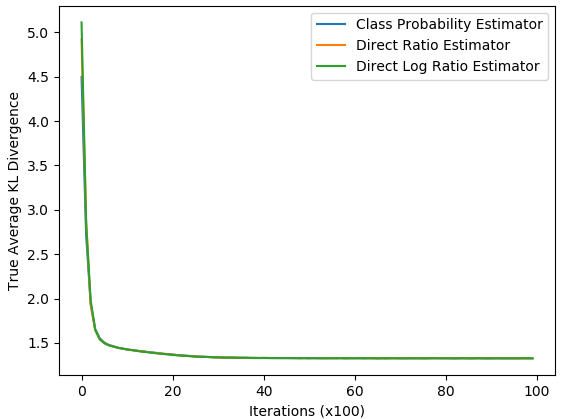
\includegraphics[width=\linewidth]{truklmins/PCADVvsPCADVexpvsPCADVgudlog.png}
\caption{GAN Divergence}
\end{subfigure}
\begin{subfigure}{0.33\textwidth}
\centering
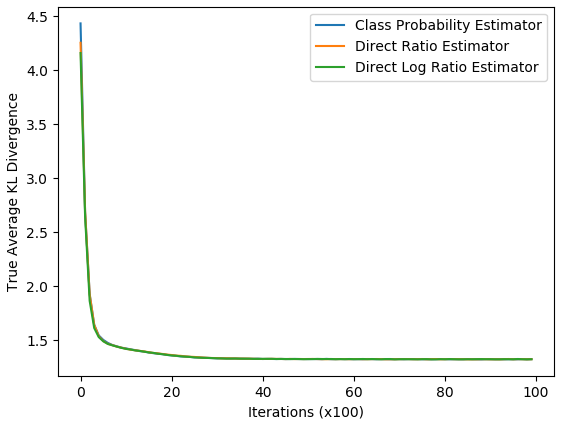
\includegraphics[width=\linewidth]{truklmins/PCKLDvsPCKLexpvsPCKLgudlog.png}
\caption{Reverse KL Divergence}
\end{subfigure}
\caption{Prior-Contrastive Average KL Divergence}
\end{figure}
\vspace*{-0.6cm}
\begin{figure}[h]
\centering
\begin{subfigure}{0.33\textwidth}
\centering
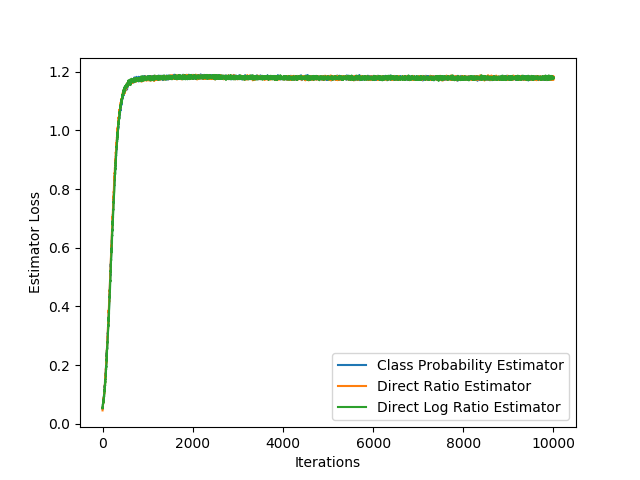
\includegraphics[width=\linewidth]{estimator_losses/PCADVvsPCADVexpvsPCADVgudlog.png}
\caption{GAN Divergence}
\end{subfigure}
\begin{subfigure}{0.33\textwidth}
\centering
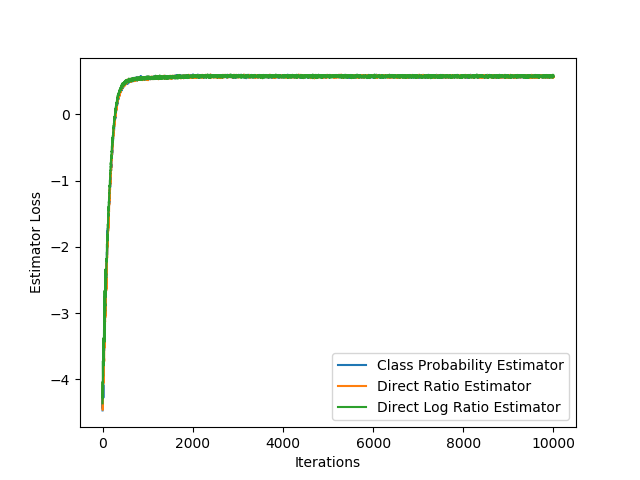
\includegraphics[width=\linewidth]{estimator_losses/PCKLDvsPCKLexpvsPCKLgudlog.png}
\caption{Reverse KL Divergence}
\end{subfigure}
\caption{Prior-Contrastive Estimator Loss}
\end{figure}
\vspace*{-0.6cm}
\begin{figure}[h]
\centering
\begin{subfigure}{0.33\textwidth}
\centering
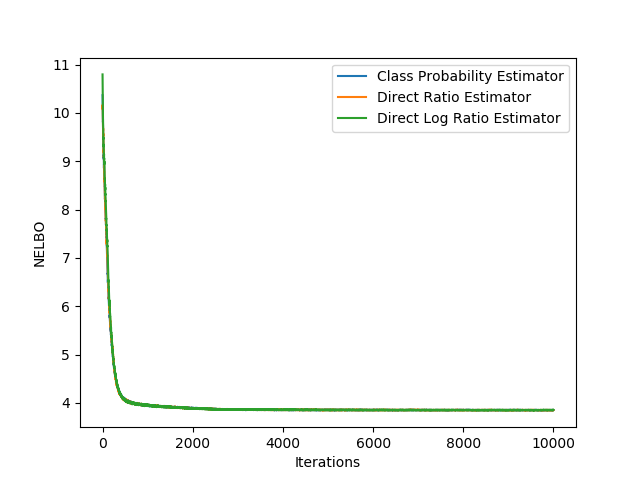
\includegraphics[width=\linewidth]{nelbos/PCADVvsPCADVexpvsPCADVgudlog.png}
\caption{GAN Divergence}
\end{subfigure}
\begin{subfigure}{0.33\textwidth}
\centering
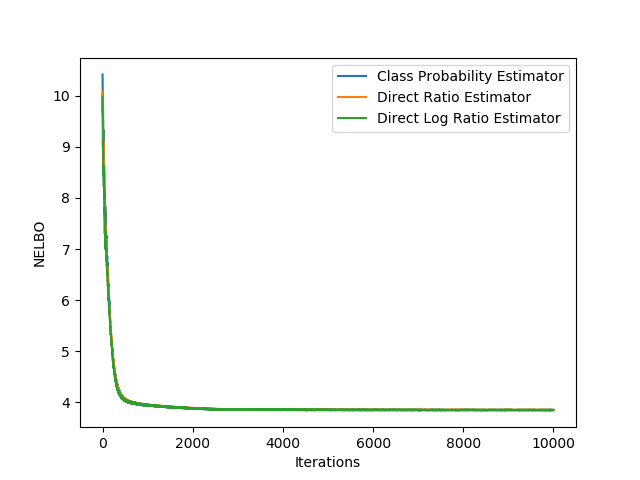
\includegraphics[width=\linewidth]{nelbos/PCKLDvsPCKLexpvsPCKLgudlog.png}
\caption{Reverse KL Divergence}
\end{subfigure}
\caption{Prior-Contrastive $NELBO$}
\end{figure}
\chapter{Second Functional Derivatives of Direct Log Ratio Estimator Losses}\label{app:F}
\textbf{Reverse KL Divergence Bound}\\
Direct Log Ratio Estimator:
\begin{align*}
L_{RKL}(u)&\coloneqq-\E_{q(u)}[T_\alpha(u)]+\E_{p(u)}\left[e^{T_\alpha(u)}\right]\\
&=-\int_U q(u)T_\alpha(u)\, {\rm d}u+\int_U p(u)e^{T_\alpha(u)}\, {\rm d}u.\\
\frac{\partial L_{RKL}(u)}{\partial T_\alpha(u)}&=-q(u)+p(u)e^{T_\alpha(u)}.\\
\frac{\partial^2L_{RKL}(u)}{\partial T_\alpha^2(u)}&=p(u)e^{T_\alpha(u)}.
\end{align*}
\textbf{GAN Divergence Bound}\\
Direct Log Ratio Estimator:
\begin{align*}
L_{GAN}(u)&\coloneqq-\E_{q(u)}\left[T_\alpha(u)-\log\left(e^{T_\alpha(u)}+1\right)\right]+\E_{p(u)}\left[\log\left(e^{T_\alpha(u)}+1\right)\right]\\
&=\int_U q(u)\left[\log\left(e^{T_\alpha(u)}+1\right)-T_\alpha(u)\right] \, {\rm d}u+\int_U p(u)\left[\log\left(e^{T_\alpha(u)}+1\right)\right]\, {\rm d}u.\\
\frac{\partial L_{GAN}(u)}{\partial T_\alpha(u)}&=-q(u)+\frac{(q(u)+p(u))e^{T_\alpha(u)}}{e^{T_\alpha(u)}+1}.\\
\frac{\partial^2L_{GAN}(u)}{\partial T_\alpha^2(u)}&=\frac{(q(u)+p(u))e^{T_\alpha(u)}}{e^{T_\alpha(u)}+1}-\frac{(q(u)+p(u))e^{2T_\alpha(u)}}{(e^{T_\alpha(u)}+1)^2}\\
&=\frac{(q(u)+p(u))(e^{2T_\alpha(u)}+e^{T_\alpha(u)})-(q(u)+p(u))e^{2T_\alpha(u)}}{(e^{T_\alpha(u)}+1)^2}\\
&=\frac{(q(u)+p(u))e^{T_\alpha(u)}}{(e^{T_\alpha(u)}+1)^2}.
\end{align*}
\end{document}





